\begin{figure}
\centering
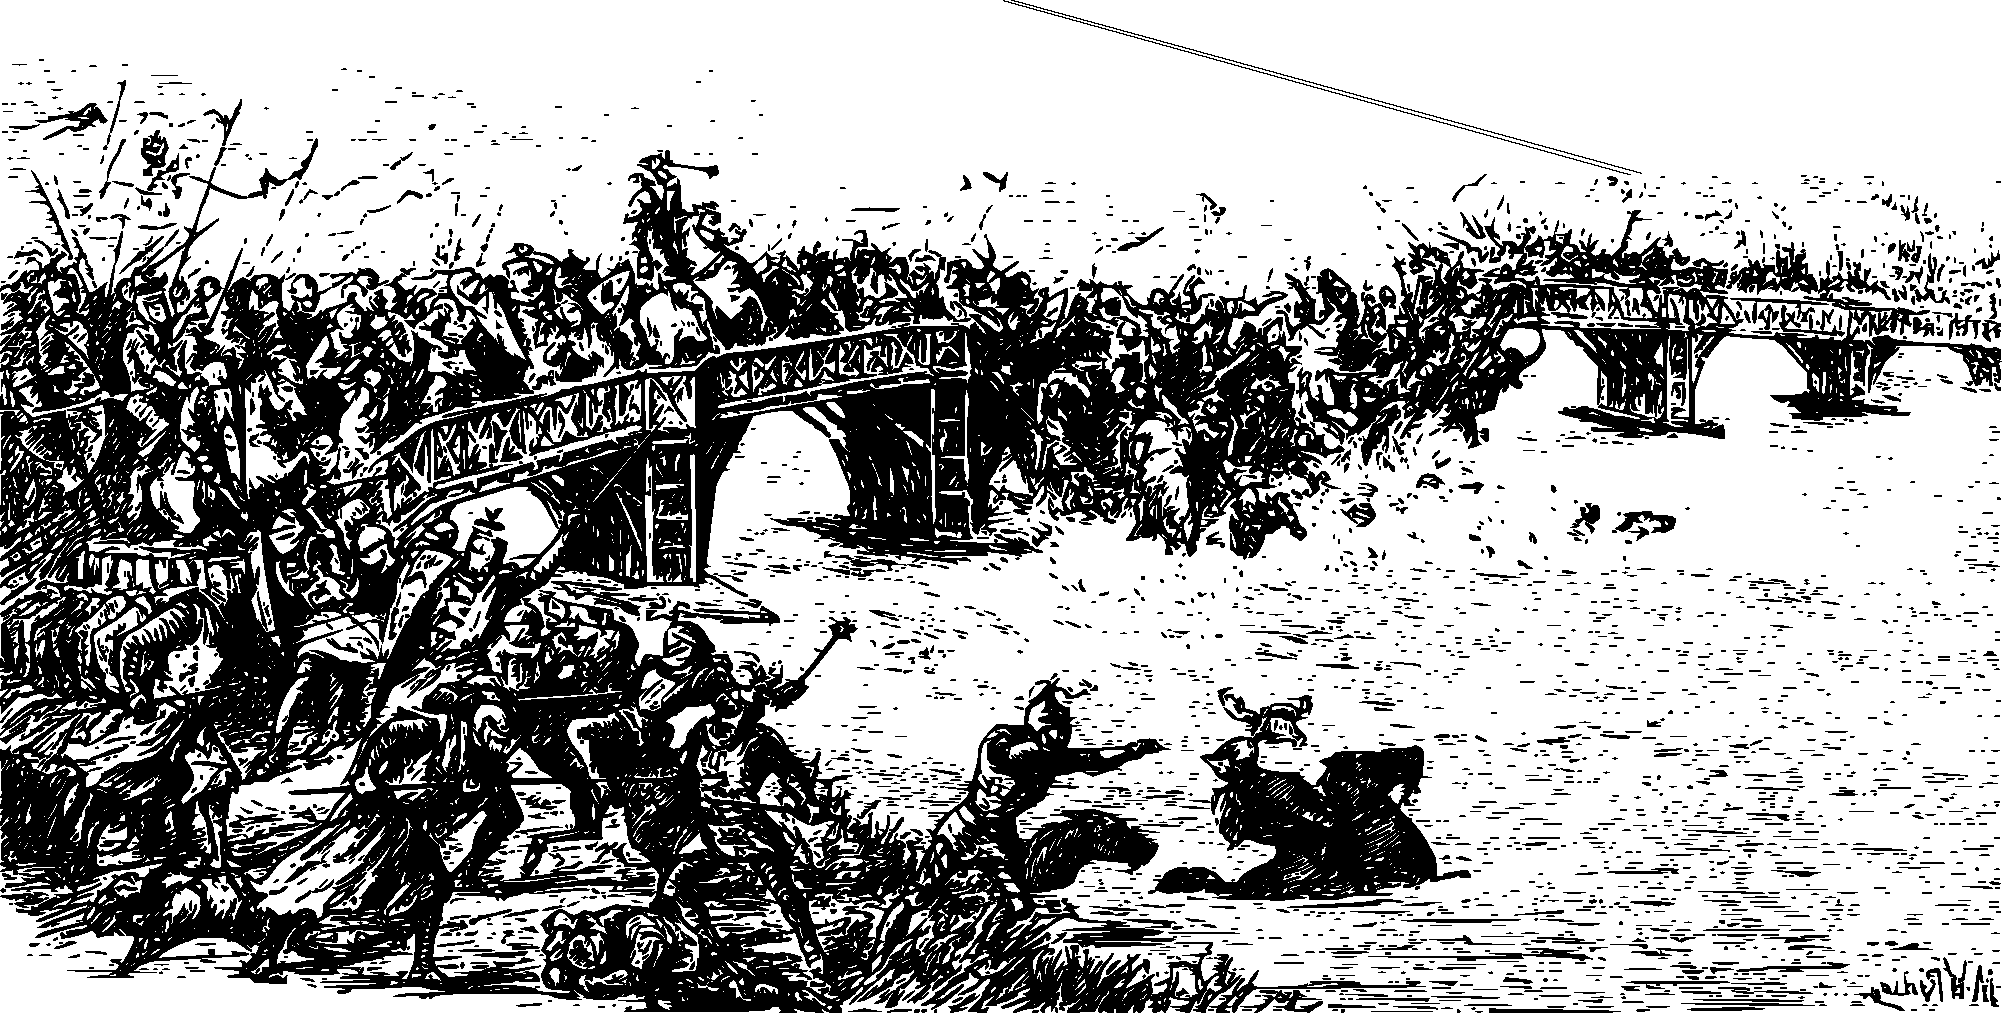
\includegraphics{./images/index01.pdf}
\caption{Image1}
\end{figure}

\hypertarget{presentation}{%
\section{Presentation}\label{presentation}}

In the realm of tabletop role-playing games, Eidos stands as a unique
and innovative addition to the genre. Rooted in the principles of open
source development, this game is designed to be both immersive and
accessible, offering a deep and rich narrative experience that is driven
by player choice. Eidos takes its name from the ancient Greek concept of
the world of ideas, reflecting the game's focus on immersive and
thought-provoking narratives. This name is a nod to the idea that in
role-playing games, players have the ability to explore and interact
with an imagined world filled with endless possibilities.

The character creation process in Eidos is a deep and engaging
experience, allowing players to build their characters from the ground
up. With character sheets devoted to personality, religion, physical
description, background, clothing, equipment, and skills, players have
the tools to create a truly unique and memorable character.

The combat system in Eidos is designed to be immersive and engaging,
with mechanics that are designed to create dynamic and exciting combat
scenes. The game's mechanics are based on classic combat narratives, and
the system strives to be a simulation of combat rather than simply a
turn-based dice-rolling game. The standard rules are designed to be
played in a pre-modern low-fantasy setting, but the game is easily
adaptable to other role-playing scenarios.

This rulebook is divided into six chapters, each of which covers a
different aspect of the game. Chapter 1: Character Creation provides a
detailed guide to creating your character, including sections on
personality, religion, physical description, background, clothing,
equipment, and skills. Chapter 2: Combat and Combat Resolution covers
the mechanics of combat in Eidos, including basic combat mechanics,
ability checks, skills, tactical maneuvering, environmental interaction,
morale, reinforcements, ranged combat, unarmed combat, weapon mechanics,
grappling, healing, shields and armor, mounted combat, naval combat,
aerial combat, siege weapons, traps, stealth, mass combat, and death and
dying.

\begin{figure}
\centering
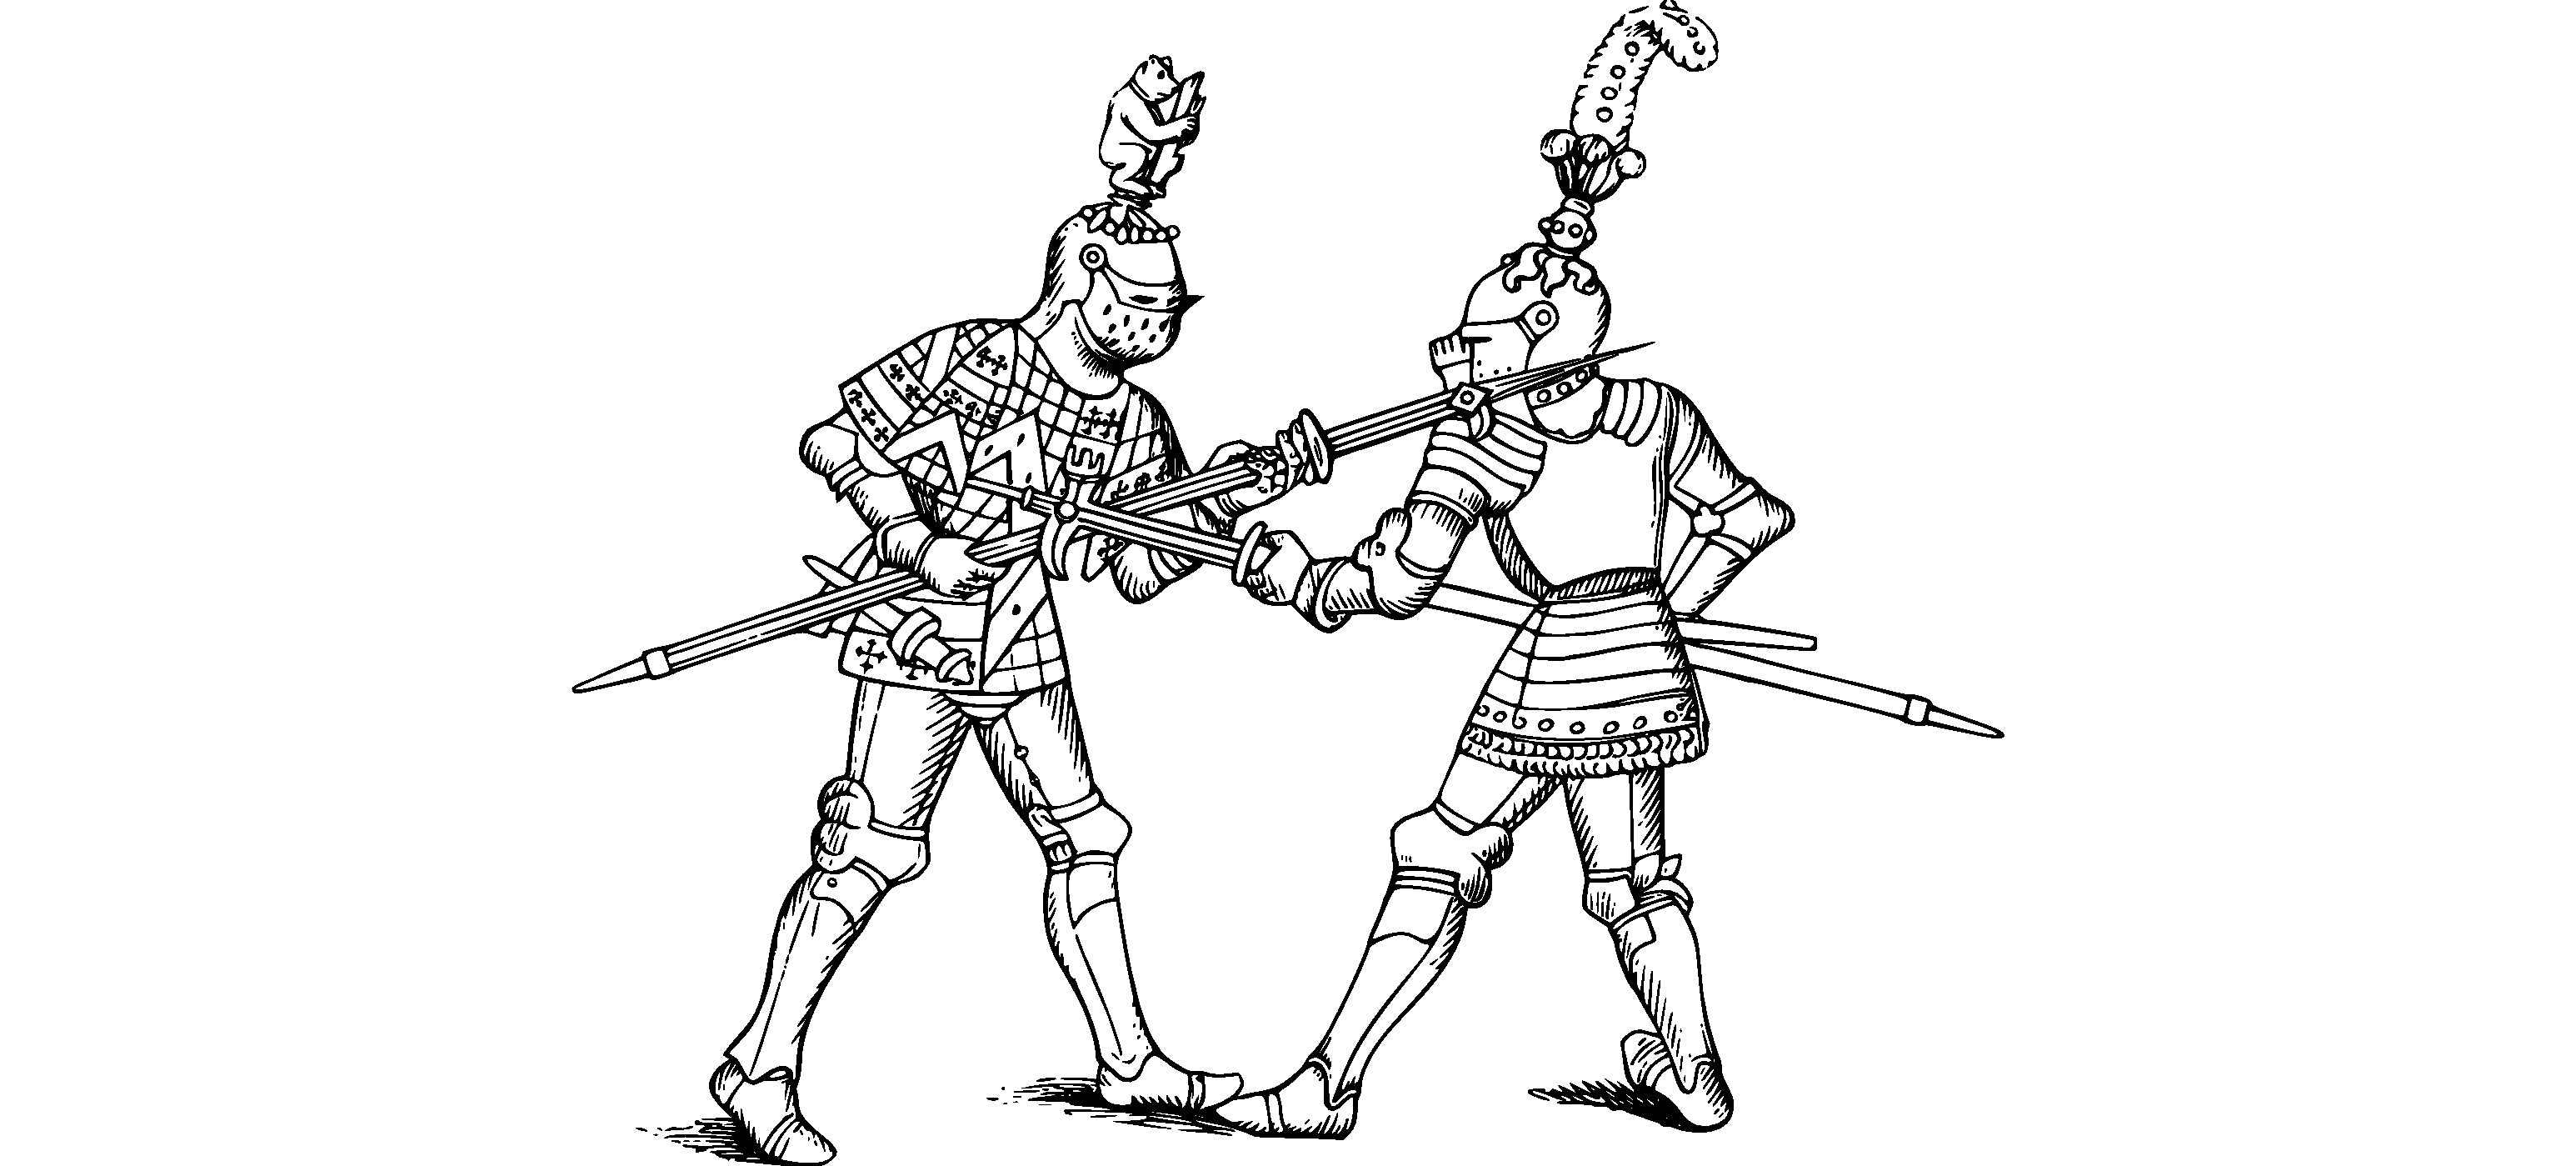
\includegraphics{./images/index02.pdf}
\caption{Image1}
\end{figure}

Chapter 3: Survival Mechanics covers the mechanics of survival in Eidos,
including food and water requirements, shelter, scavenging, travel, and
exploration. Chapter 4: Character Injuries and Health provides a
comprehensive guide to character injuries and health, including damage
and wound mechanics, healing and recovery, status effects, and advanced
injuries and trauma.

Chapter 5: Game Master Tools provides a guide to running Eidos games,
including world-building, NPC generation, encounters, group dynamics,
movement and travel, encounter generation, and campaign management.
Chapter 6: Optional Rules and Variants covers alternative systems for
combat, magic, and skills, as well as advanced mechanics for character
development and progression and rules for playing in different settings
and genres.

In conclusion, Eidos is an open source tabletop RPG system that offers a
unique and engaging narrative experience, with mechanics that are
designed to create immersive and exciting combat scenes. With its deep
character creation process, engaging combat mechanics, and comprehensive
survival mechanics, Eidos is a game that offers endless possibilities
for players to explore and experience.

\hypertarget{personality}{%
\section{Personality}\label{personality}}

\begin{figure}
\centering
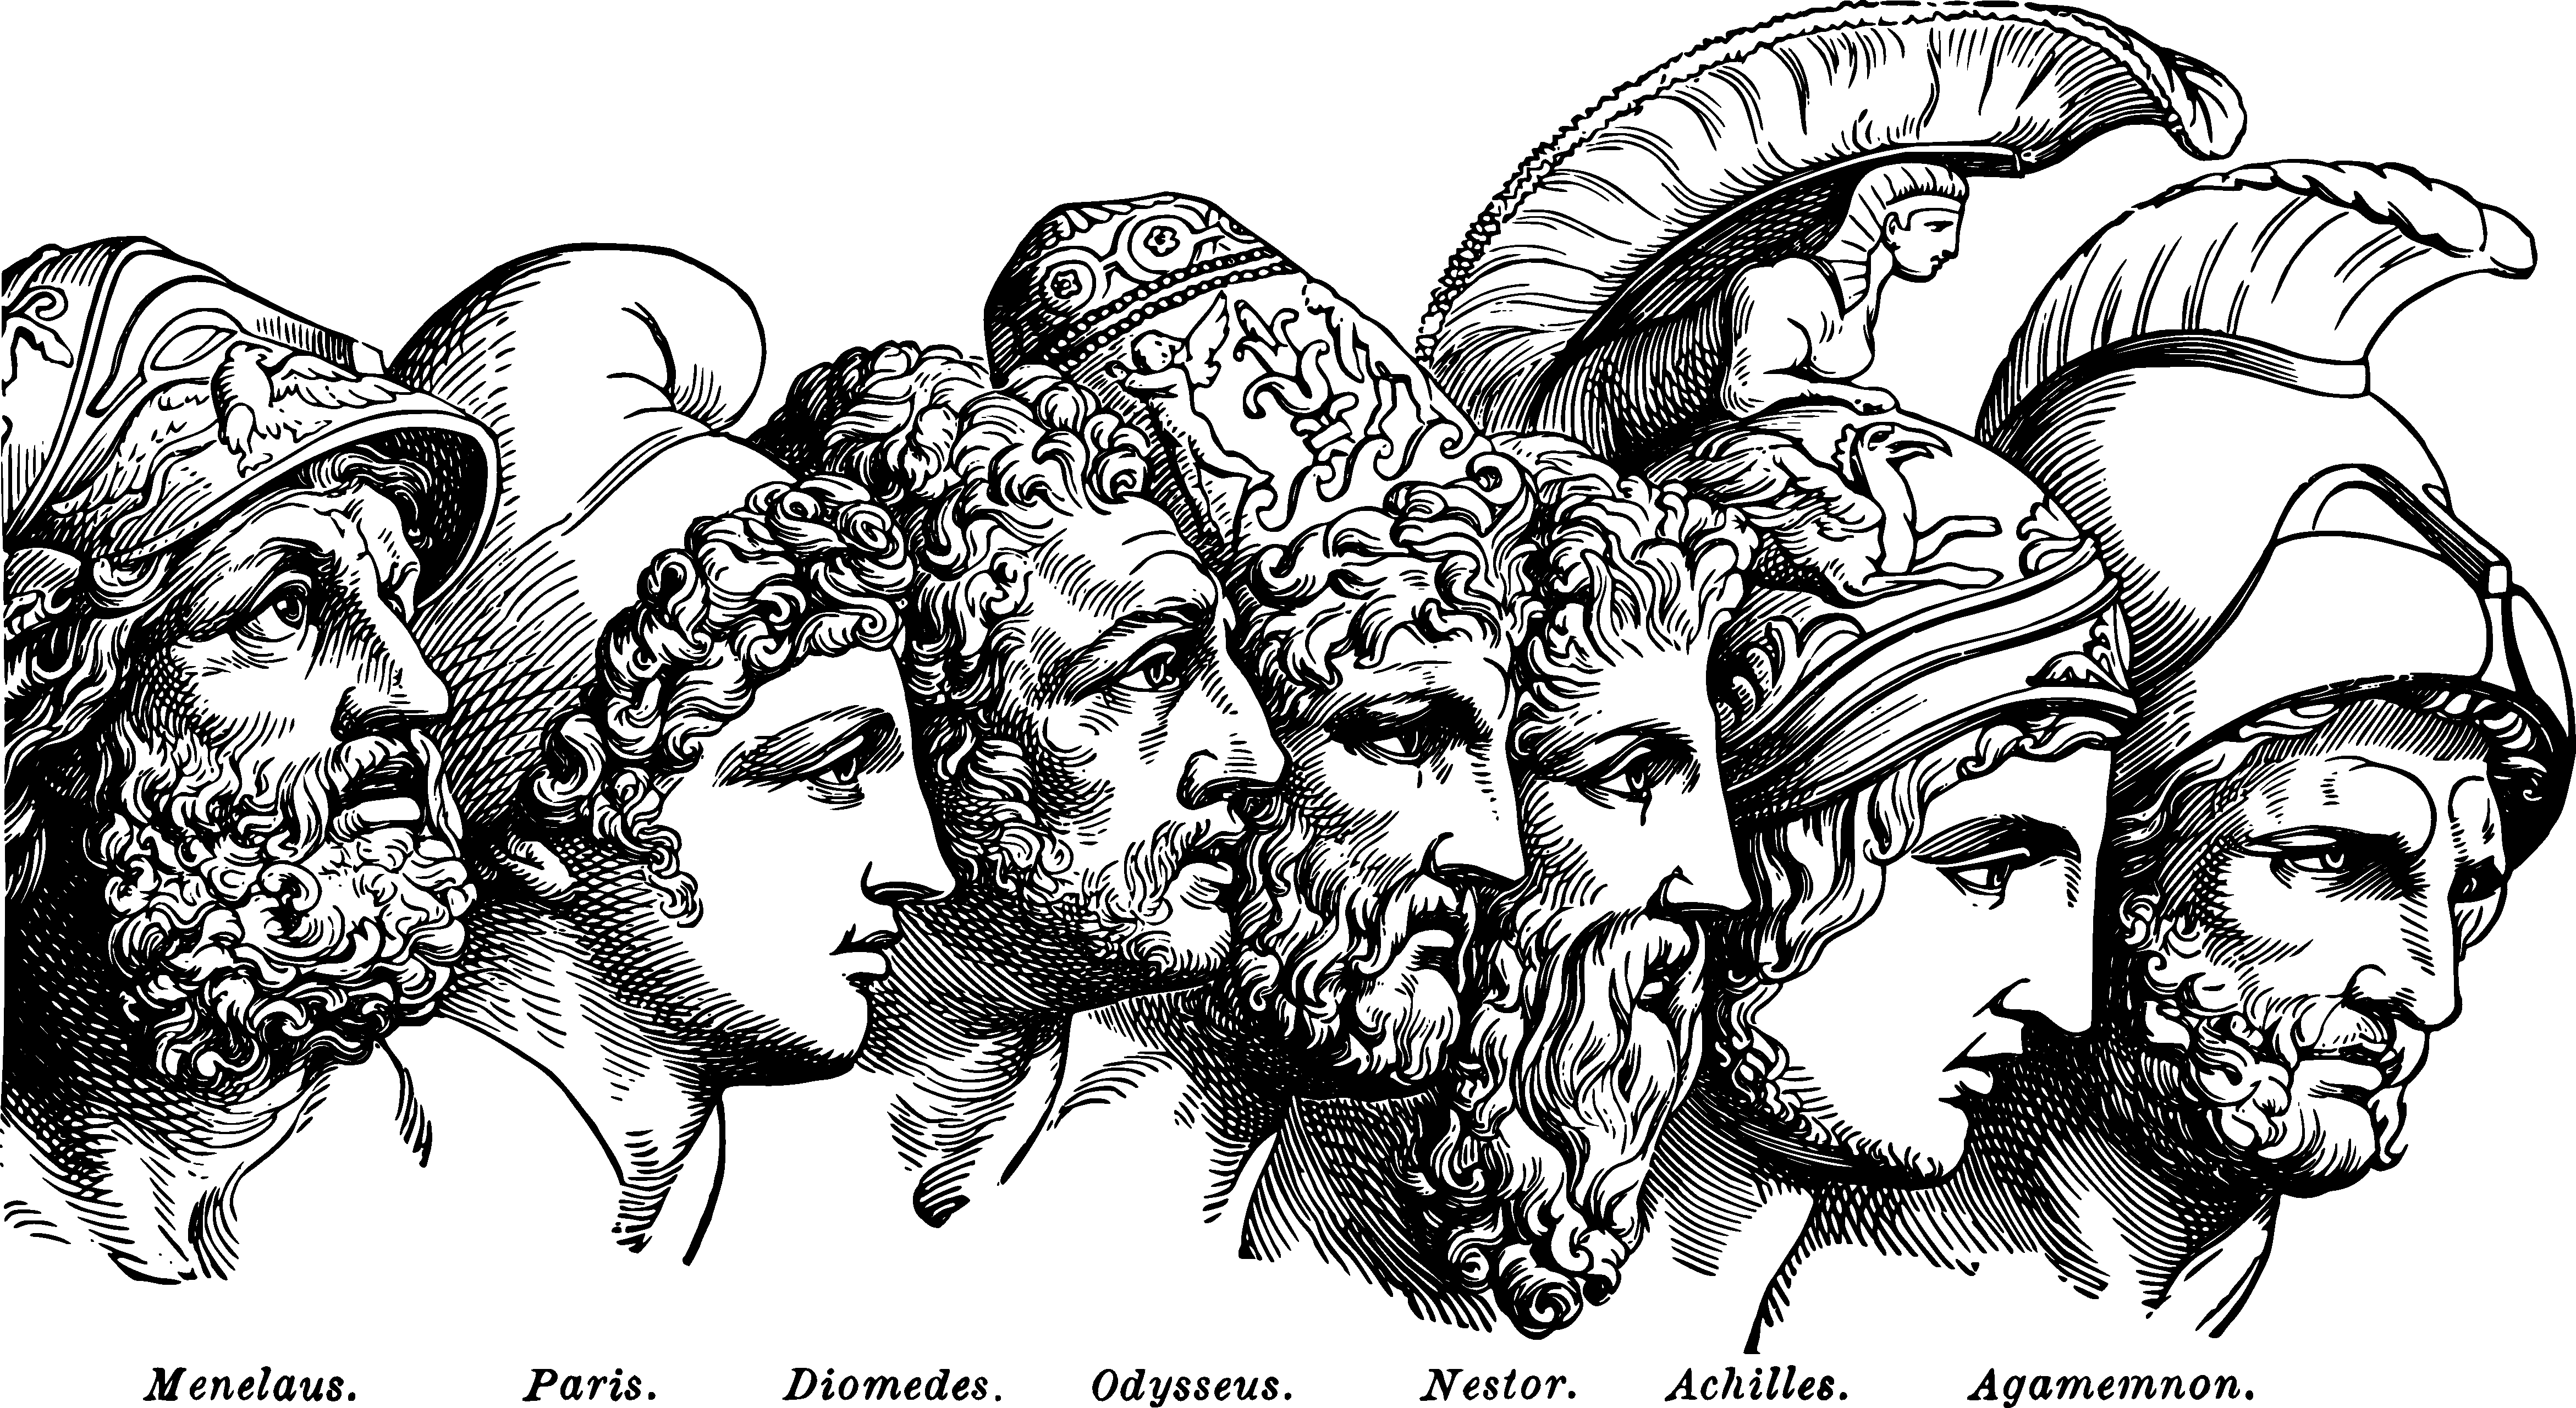
\includegraphics{./images/personality01.pdf}
\caption{Image1}
\end{figure}

Most of this part will be based in the
\href{https://www.ashami.com/rpg/}{Ash's Guide to RPG Personality \&
Background}. Of course it its not a carbon copie, some modifications
will be needed to fit his tables in the system. Anyway, credits must be
given and you should check out his guide.

\hypertarget{primary-motivators}{%
\subsection{Primary Motivators}\label{primary-motivators}}

The first step in crafting a character's personality is selecting their
primary and secondary motivators. These motivations serve as the driving
force behind a character's actions and decisions, shaping the narrative
of their journey. The primary motivator is particularly important, as it
acts as the primary catalyst for a character's backstory and
personality. It is the underlying theme of a character's motivations,
guiding their behavior and propelling them forward.

When choosing these motivations, it's important to consider what your
character wants most in the world. Is it wealth, power, love, revenge,
or something else? By focusing on these motivations, players can ensure
that their character's actions feel authentic and grounded in their
personal desires. Whether facing challenges in combat or navigating
complex social situations, characters driven by strong motivators will
always have a clear direction and purpose.

\begin{longtable}[]{@{}
  >{\raggedright\arraybackslash}p{(\columnwidth - 4\tabcolsep) * \real{0.0291}}
  >{\raggedright\arraybackslash}p{(\columnwidth - 4\tabcolsep) * \real{0.1845}}
  >{\raggedright\arraybackslash}p{(\columnwidth - 4\tabcolsep) * \real{0.7864}}@{}}
\toprule
\begin{minipage}[b]{\linewidth}\raggedright
No.
\end{minipage} & \begin{minipage}[b]{\linewidth}\raggedright
Theme
\end{minipage} & \begin{minipage}[b]{\linewidth}\raggedright
Description
\end{minipage} \\
\midrule
\endhead
1 & Achievement & To overcome obstacles and succeed; to become the
best \\
2 & Acquisition & To obtain possessions/wealth \\
3 & Adoration & To be cherished, admired, and wanted by others \\
4 & Balance/Peace & To bring all things into harmony and equilibrium \\
5 & Beneficence & To protect the helpless, heal the sick, feed the
hungry, etc. \\
6 & Chaos & To disrupt, to cause confusion and discord \\
7 & Competition & To seek out or create rule-based win/lose scenarios;
to defeat others in contests \\
8 & Conflict & To seek out or create rivalry, fighting, or animosity \\
9 & Conquest & To conquer other peoples, to bring them into one's own
culture/rule \\
10 & Corruption & To despoil, ruin, humiliate, or make depraved \\
11 & Creation & To build or make new, such as art, culture, invention,
design, etc. \\
12 & Destruction & To annihilate, exterminate, and unmake \\
13 & Discovery/Adventure & To explore, uncover mysteries, and pioneer \\
14 & Domesticity & To get married, have children, and live a family
life \\
15 & Education & To provide information, teach, enlighten, or train \\
16 & Entertainment & To entertain, amuse, and delight others \\
17 & Enslavement & To force others into servitude \\
18 & Hedonism & To enjoy all things sensuous \\
19 & Heroism & To find valor and honor through battle or
self-sacrifice \\
20 & Liberation & To free the self and/or others from perceived
captivity or enslavement \\
21 & Love & To experience/share affection and emotional commitment,
romantic or platonic \\
22 & Nobility/Honor & To exalt ideals such as generosity, honesty,
bravery, and courtliness \\
23 & Order & To arrange, organize, and reduce chaos \\
24 & Play & To have fun, to enjoy life \\
25 & Power & To control and lead others \\
26 & Proselytization & To spread a belief system; indoctrinate others \\
27 & Purity & To achieve a state of moral or spiritual perfection, of
self and/or others \\
28 & Rebellion & To fight against power structures; to undermine
authority \\
29 & Recognition & To gain approval, social status, or fame \\
30 & Service & To follow a person, government, order, religion, etc. \\
31 & Torment & To inflict pain and suffering, on others and/or the
self \\
32 & Understanding & To seek knowledge or wisdom (spiritual, scientific,
magical, etc) \\
33 & Vice & To enable or engage in self-destructive behavior \\
\bottomrule
\end{longtable}

\begin{figure}
\centering
\includegraphics{./images/personality02.pdf}
\caption{Image}
\end{figure}

\hypertarget{dispositions}{%
\subsection{Dispositions}\label{dispositions}}

Disposition is an important aspect of character creation that provides
depth and dimension to your character's personality. It allows you to
understand how your character is likely to react emotionally to
different situations, as well as how they appear to others. This trait
helps you create a believable and relatable character, giving them an
emotional landscape that makes sense within the context of the story.

When determining your character's emotional disposition, it is important
to keep in mind that it is not necessarily limiting. It simply provides
a baseline for how your character is likely to feel at any given moment.
A character with a predominantly cheerful disposition may still
experience moments of sadness, anger, or anxiety, but they will be more
likely to return to their cheerful state after those moments have
passed.

It is also important to note that emotional disposition should not be
equated with alignment. A character's disposition can exist
independently of their moral or ethical alignment, and it is possible
for a character to be joyfully evil or angrily good. Understanding your
character's disposition will help you make decisions about their
emotional reactions, but it is just one aspect of the complex and
multifaceted personality that you are creating.

\begin{enumerate}
\def\labelenumi{\arabic{enumi}.}
\tightlist
\item
  Joyful
\item
  Anxious
\item
  Melancholy
\item
  Curious
\item
  Calm
\item
  Angry
\item
  Contemptuous
\item
  Excited
\item
  Apathetic
\item
  Ashamed
\end{enumerate}

\hypertarget{moodiness}{%
\subsection{Moodiness}\label{moodiness}}

Moodiness is an important aspect of a character's personality and can
greatly impact their behavior in different situations. A character who
is labile, or quick to experience intense emotions, is likely to react
strongly to the events happening around them. This can make them appear
impulsive and prone to outbursts, but it can also add a level of
excitement and unpredictability to their actions. On the other hand, a
phlegmatic character, who is psychologically consistent and moderate, is
likely to maintain their composure in even the most trying of
situations. This calm demeanor can give them a sense of stability and
reliability, but it can also make them appear uninterested or
indifferent to the world around them.

It is important to note that both moodiness traits have their own
strengths and weaknesses, and they can greatly impact a character's
relationships with other characters. For example, a labile character may
be prone to jealousy or resentment, while a phlegmatic character may
struggle with expressing their emotions effectively. Choosing the right
moodiness trait for your character can help you build a more complete
and well-rounded personality.

Ultimately, the key to making a character's moodiness work for them is
understanding the underlying motivations and dispositions that drive
their behavior. Whether your character is quick to experience intense
emotions or stays calm and collected in the face of adversity, the key
is to make sure that their moodiness feels true to who they are as a
character. By incorporating moodiness into your character's personality,
you can add depth and richness to your role-playing experience and help
bring your character to life on the tabletop.

\begin{enumerate}
\def\labelenumi{\arabic{enumi}.}
\tightlist
\item
  Labile
\item
  Even-tempered
\item
  Phlegmatic
\end{enumerate}

\begin{figure}
\centering
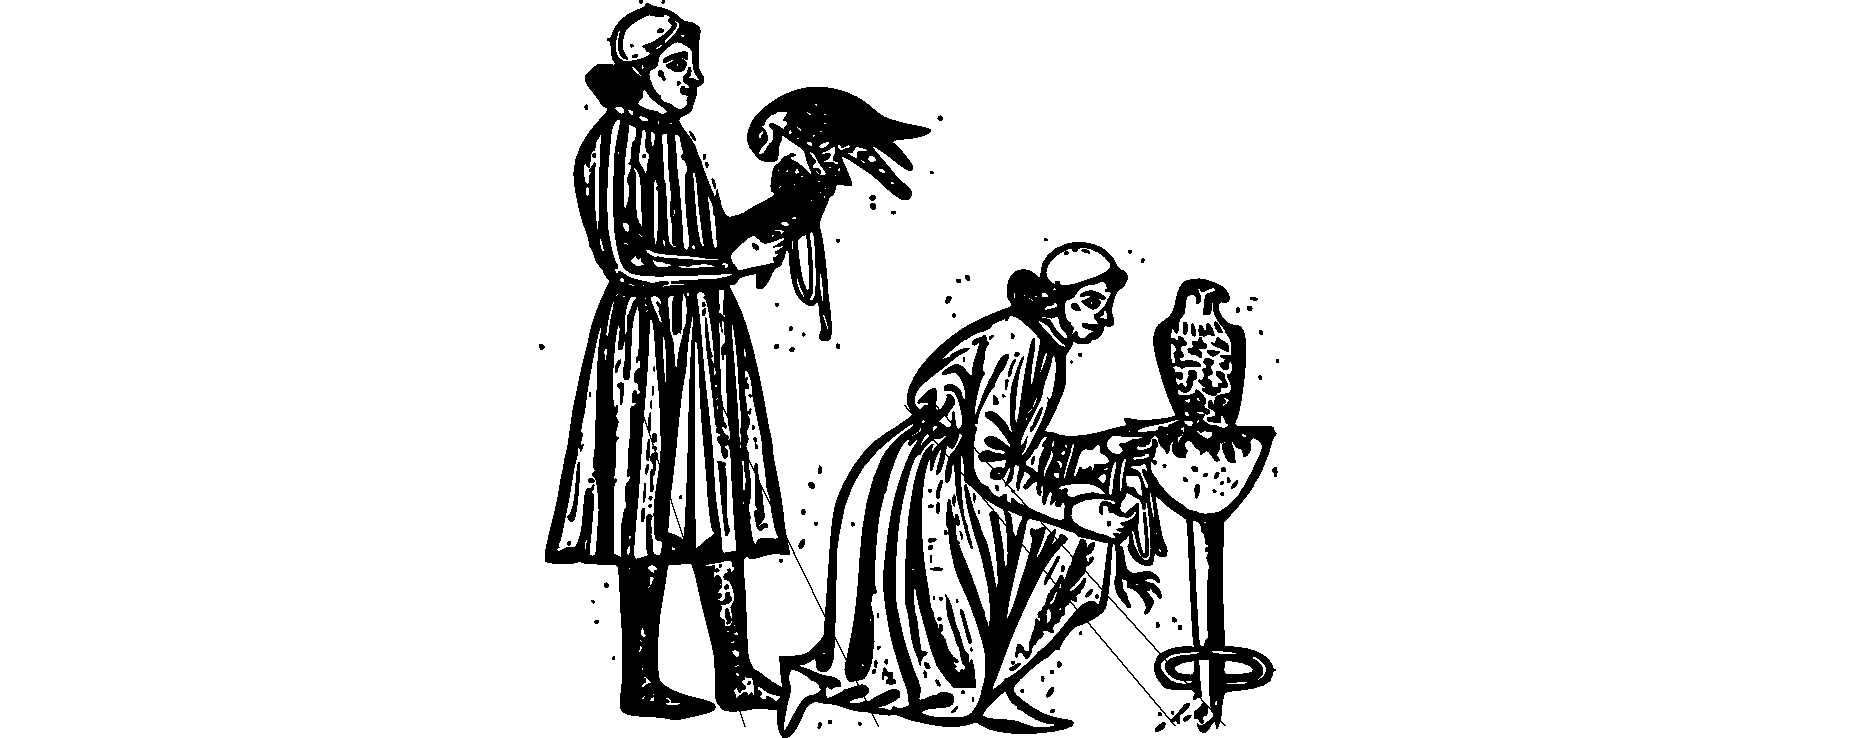
\includegraphics{./images/personality03.pdf}
\caption{Image1}
\end{figure}

\hypertarget{outlook}{%
\subsection{Outlook}\label{outlook}}

The concept of outlook is an important aspect of character creation as
it defines the basic worldview of a character and helps determine their
overall view of the world around them. This trait can greatly influence
the choices that a character makes and the way they interact with
others. A character with a positive outlook is likely to see the good in
people and situations, while a character with a negative outlook is
likely to be more skeptical and pessimistic. Understanding a character's
outlook is key to understanding their motivations and how they may react
in different situations. It is important to note that a character's
outlook does not dictate their alignment, as a character can have a
positive outlook but still make morally questionable decisions. This
trait helps to add depth and complexity to a character, making them feel
more real and unique.

\begin{longtable}[]{@{}ll@{}}
\toprule
Outlook & Description \\
\midrule
\endhead
Optimistic & Idealistic, confident, trusting, hopeful, upbeat \\
Pessimistic & Cynical, bleak, distrustful, foreboding, resigned \\
\bottomrule
\end{longtable}

\hypertarget{integrity}{%
\subsection{Integrity}\label{integrity}}

Integrity refers to the values that guide a character's behavior in work
and social interactions. When creating a character, players can choose
between two options that embody different qualities and tendencies. The
first option is ``Conscientious'', which represents being industrious,
honest, responsible, meticulous, and pragmatic. On the other hand, the
second option is ``Unscrupulous'', which embodies being lazy, deceitful,
unreliable, manipulative, slipshod, and impractical. These two options
serve as a starting point for players to develop their character's
personality and decision-making. The choice of integrity will play a
crucial role in determining a character's motivations and actions,
influencing the character's interactions with others and the events of
the story.

\begin{longtable}[]{@{}
  >{\raggedright\arraybackslash}p{(\columnwidth - 2\tabcolsep) * \real{0.1688}}
  >{\raggedright\arraybackslash}p{(\columnwidth - 2\tabcolsep) * \real{0.8312}}@{}}
\toprule
\begin{minipage}[b]{\linewidth}\raggedright
Integrity
\end{minipage} & \begin{minipage}[b]{\linewidth}\raggedright
Description
\end{minipage} \\
\midrule
\endhead
Conscientious & Industrious, honest, responsible, meticulous,
pragmatic \\
Unscrupulous & Lazy, deceitful, unreliable, manipulative, slipshod,
impractical \\
\bottomrule
\end{longtable}

\begin{figure}
\centering
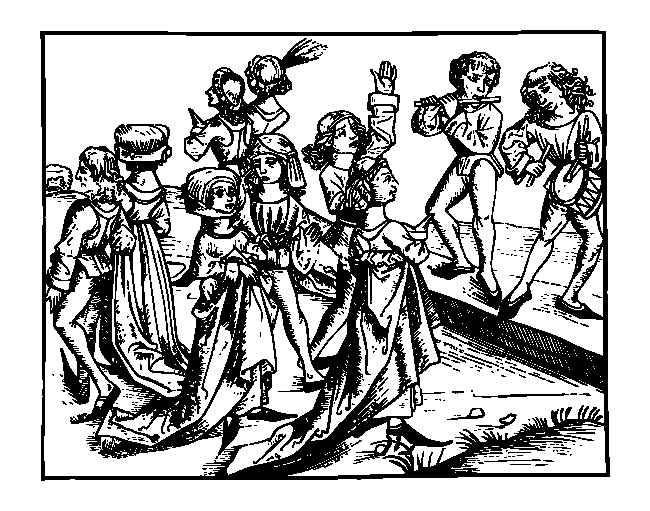
\includegraphics{./images/personality04.pdf}
\caption{Image1}
\end{figure}

\hypertarget{impulsiveness}{%
\subsection{Impulsiveness}\label{impulsiveness}}

The next aspect of character creation to consider is impulsiveness. This
trait refers to a character's ability to regulate their thoughts and
actions. Players must choose between two options: controlled or
spontaneous. A controlled character is deliberate, focused, steady, and
thoughtful. They carefully consider their decisions and think before
they act. On the other hand, a spontaneous character is capricious,
flighty, hyperactive, and rash. They are quick to act without thinking
through the consequences of their actions. It's important to consider
impulsiveness as it can greatly impact the way a character approaches
situations and reacts to stimuli. A controlled character may be more
reliable and level-headed, while a spontaneous character may be more
unpredictable and exciting. Ultimately, the choice of impulsiveness
helps to round out a character's personality and inform their behavior.

\begin{longtable}[]{@{}ll@{}}
\toprule
Impulsiveness & Description \\
\midrule
\endhead
Controlled & Deliberate, focused, steady, thoughtful \\
Spontaneous & Capricious, flighty, hyperactive, rash \\
\bottomrule
\end{longtable}

\hypertarget{boldness}{%
\subsection{Boldness}\label{boldness}}

When it comes to creating a character's personality, it is important to
consider their boldness, or willingness to face danger and enter into
battle. This trait can greatly impact how a character approaches
conflict and adversity, and can inform their actions and decisions in
high-pressure situations. There are two main options for this
characteristic: intrepid and cautious.

Intrepid characters are daring, reckless, and valorous. They have a
confident demeanor and are not easily intimidated by danger. They are
known for their bravery and audacity in the face of adversity, and are
often seen as leaders in combat situations. On the other hand, cautious
characters are timid, paranoid, and vigilant. They are nervous and
tentative in the face of danger, preferring to assess the situation
before making a move. They are not as quick to jump into action, but
their carefulness can often lead to a more strategic approach to
conflict.

\begin{longtable}[]{@{}
  >{\raggedright\arraybackslash}p{(\columnwidth - 2\tabcolsep) * \real{0.1194}}
  >{\raggedright\arraybackslash}p{(\columnwidth - 2\tabcolsep) * \real{0.8806}}@{}}
\toprule
\begin{minipage}[b]{\linewidth}\raggedright
Boldness
\end{minipage} & \begin{minipage}[b]{\linewidth}\raggedright
Description
\end{minipage} \\
\midrule
\endhead
Intrepid & Daring, reckless, valorous, dauntless, audacious,
confident \\
Cautious & Timid, paranoid, vigilant, nervous, tentative \\
\bottomrule
\end{longtable}

\begin{figure}
\centering
\includegraphics{./images/personality05.pdf}
\caption{Image1}
\end{figure}

\hypertarget{agreeableness}{%
\subsection{Agreeableness}\label{agreeableness}}

The sub-topic of ``Agreeableness'' deals with a character's overall
attitude towards others and their ability to handle interpersonal
conflicts and new situations. This trait is particularly important in
shaping a character's behavior in social interactions and their ability
to navigate challenging circumstances. A character who is described as
``Agreeable'' is warm, empathetic, and open-minded, possessing qualities
such as tolerance, forgiveness, and adaptability. On the other hand, a
character who is described as ``Disagreeable'' is cold and rigid,
possessing traits such as tension, intractability, and
narrow-mindedness. Understanding a character's level of agreeableness
can give insight into how they are likely to respond in social and
interpersonal situations.

\begin{longtable}[]{@{}
  >{\raggedright\arraybackslash}p{(\columnwidth - 2\tabcolsep) * \real{0.1548}}
  >{\raggedright\arraybackslash}p{(\columnwidth - 2\tabcolsep) * \real{0.8452}}@{}}
\toprule
\begin{minipage}[b]{\linewidth}\raggedright
Agreeableness
\end{minipage} & \begin{minipage}[b]{\linewidth}\raggedright
Description
\end{minipage} \\
\midrule
\endhead
Agreeable & Warm, empathic, tolerant, forgiving, open-minded, adaptable,
altruistic \\
Disagreeable & Cold, rigid, tense, intractable, narrow-minded,
cantankerous, stingy \\
\bottomrule
\end{longtable}

\hypertarget{interactivity}{%
\subsection{Interactivity}\label{interactivity}}

The next sub-topic in character creation is Interactivity, which deals
with the way your character interacts with others. This aspect of
personality is crucial in shaping the character's social relationships
and determining how they engage with the world around them. The table of
choices in Interactivity includes two options: Engaging and Reserved. An
Engaging character is often talkative, candid, and touchy, while a
Reserved character is usually shy, preferring to keep to themselves and
be more reserved in their interactions. Understanding this aspect of
your character will greatly enhance the depth of your role-playing
experience and allow you to build compelling, engaging stories.

\begin{longtable}[]{@{}ll@{}}
\toprule
Interactivity & Description \\
\midrule
\endhead
Engaging & Talkative, candid, entertaining, touchy \\
Reserved & Shy, loner, taciturn, evasive, cryptic \\
\bottomrule
\end{longtable}

\hypertarget{conformity}{%
\subsection{Conformity}\label{conformity}}

Conformity is an important aspect of a character's personality,
determining their relationship with cultural norms and societal
expectations. A character who is conventional is likely to follow
orthodox beliefs and practices, be formal in their demeanor, and adhere
to mainstream customs. On the other hand, a character who is heterodox
may be rebellious in nature, have a creative and artistic streak, and
may be known for their freethinking and exotic choices. Understanding a
character's conformity can give insight into how they view and interact
with the world around them.

\begin{longtable}[]{@{}
  >{\raggedright\arraybackslash}p{(\columnwidth - 2\tabcolsep) * \real{0.1765}}
  >{\raggedright\arraybackslash}p{(\columnwidth - 2\tabcolsep) * \real{0.8235}}@{}}
\toprule
\begin{minipage}[b]{\linewidth}\raggedright
Conformity
\end{minipage} & \begin{minipage}[b]{\linewidth}\raggedright
Description
\end{minipage} \\
\midrule
\endhead
Conventional & Orthodox, formal, down-to-earth, mainstream,
traditional \\
Heterodox & Rebellious, arty, shocking, freethinking, exotic \\
\bottomrule
\end{longtable}

\hypertarget{quirks-habits-and-oddities}{%
\subsection{Quirks, Habits, and
Oddities}\label{quirks-habits-and-oddities}}

To help bring your character to life and add depth to gameplay, consider
incorporating small quirks, habits, and oddities into their personality.
These unique behavioral characteristics can range from relatively
harmless habits, such as humming or lip biting, to more engaging and
potentially entertaining quirks such as exhibitionism or sleepwalking.
By adding these small but meaningful details to your character, you can
bring them to life in a way that sets them apart from the rest of the
party.

These quirks, habits, and oddities can offer a multitude of role-playing
opportunities. They can help flesh out a character's backstory, provide
unique challenges or benefits during gameplay, and even influence the
way they interact with other characters. For example, a character who is
a compulsive liar may struggle with building trust with others, while a
character who is an animal hater may have trouble working with
characters who have animal companions. Whether you choose to focus on
the more harmless or more engaging quirks, incorporating these small
behaviors into your character can greatly enhance your role-playing
experience.

\begin{longtable}[]{@{}
  >{\raggedright\arraybackslash}p{(\columnwidth - 4\tabcolsep) * \real{0.3423}}
  >{\raggedright\arraybackslash}p{(\columnwidth - 4\tabcolsep) * \real{0.3333}}
  >{\raggedright\arraybackslash}p{(\columnwidth - 4\tabcolsep) * \real{0.3243}}@{}}
\toprule
\endhead
1. Humming & 31. Snoring & 61. Clearing throat repeatedly \\
2. Dancing & 32. Walking backwards & 62. Covering mouth while
speaking \\
3. Sleepwalking & 33. Teeth sucking & 63. Fidgeting with hands \\
4. Facial tics & 34. Excessively touching others & 64. Whispering to
self \\
5. Exhibitionism & 35. Substance use (non-addicted) & 65. Nervous nail
biting \\
6. Fingernail biting & 36. Animal hater & 66. Licking/smacking lips \\
7. Eavesdropping & 37. Insomnia & 67. Staring blankly \\
8. Daydreaming & 38. Beard/hair stroking & 68. Chewing gum \\
9. Talking in sleep & 39. Nose picking & 69. Sighing heavily \\
10. Stuttering & 40. Needless apologizing & 70. Breathing heavily \\
11. Compulsive lying & 41. Exaggeration & 71. Scratching self \\
12. Whistling & 42. Superstitious (omens, luck, etc.) & 72. Clicking
pen/tapping fingers \\
13. Name dropping & 43. Belching & 73. Swallowing hard \\
14. Self-inflict pain/injury & 44. Sleeping in odd places & 74. Clearing
throat loudly \\
15. Mumbling & 45. Repeating others & 75. Tapping feet \\
16. Constant grooming & 46. Smelling things & 76. Fidgeting with
clothing \\
17. Foot tapping & 47. Teeth picking & 77. Avoiding eye contact \\
18. Lip biting/licking & 48. Stealing & 78. Glancing around nervously \\
19. Coin flipping & 49. Tree climbing & 79. Talking too fast/slow \\
20. Chewing (e.g.~sticks, small bones) & 50. Excessive sweating & 80.
Stuttering words \\
21. Knuckle cracking & 51. Nervous laughter & 81. Twitching facial
muscles \\
22. Collects odd things & 52. Touching/tugging earlobes & 82. Rubbing
hands together \\
23. Singing & 53. Twirling hair/beard & 83. Biting cheek/tongue \\
24. Snacking (nuts, seeds, etc.) & 54. Playing with objects & 84.
Staring off into space \\
25. Reciting poetry & 55. Biting tongue/lips & 85. Nodding/shaking head
excessively \\
26. Constant eating & 56. Nail tapping & 86. Interrupting others \\
27. Pacing & 57. Constant yawning & 87. Leaning in too close \\
28. Blade sharpening & 58. Blinking excessively & 88. Speaking loudly \\
29. Counting & 59. Bouncing legs & 89. Repeating words/phrases \\
30. Hair pulling & 60. Skipping/hopping & 90. Rocking back and forth. \\
\bottomrule
\end{longtable}

\begin{figure}
\centering
\includegraphics{./images/personality06.pdf}
\caption{Image1}
\end{figure}

\hypertarget{sense-of-humor}{%
\subsection{Sense of Humor}\label{sense-of-humor}}

Sense of Humor is an important aspect of a character's personality and
can be used to show their humor preferences and how they might react in
different situations. It ranges from crude humor to dry wit and includes
various styles such as slapstick, jokey, cynical, prankster,
mean-spirited, gleeful, and surreal. By selecting one of these options,
you can help to define your character's sense of humor and how they
might react in different situations. Having a strong sense of humor can
also be a way for your character to diffuse tense situations, and can be
used to show their lighter side. Ultimately, your character's sense of
humor is a tool that you can use to further develop their personality
and bring them to life in your storytelling.

\begin{enumerate}
\def\labelenumi{\arabic{enumi}.}
\tightlist
\item
  Crude
\item
  Dry
\item
  Slapstick
\item
  Jokey
\item
  Cynical
\item
  Prankster
\item
  Mean-spirited
\item
  Gleeful
\item
  Surreal
\end{enumerate}

\hypertarget{mental-disorders}{%
\subsection{Mental Disorders}\label{mental-disorders}}

In this RPG system, we aim to provide an accurate representation of
human mental and emotional disorders. While we understand that not all
players may want their character to struggle with such issues, it does
present an opportunity for unique and interesting role-play. For this
reason, we suggest that players consider assigning these disorders to
non-player characters, adding depth and complexity to the game world.
It's important to note that the list provided is not exhaustive and only
offers brief descriptions. Nevertheless, these disorders can also serve
as inspiration for creating realistic and terrifying curses or divine
punishments.

\textbf{Addiction}

\begin{itemize}
\tightlist
\item
  Chronic, compulsive drug/activity indulgence, despite harmful
  consequences. Can decide if it is mild, moderate, or severe.
\end{itemize}

\textbf{Amnesia}

\begin{itemize}
\tightlist
\item
  Severe memory loss; can be loss before a certain point (retrograde) or
  after (anterograde).
\end{itemize}

\textbf{Bipolar Disorder}

\begin{itemize}
\tightlist
\item
  Erratic swings from periods of mania to major depression.
\end{itemize}

\textbf{PTSD}

\begin{itemize}
\tightlist
\item
  Anxiety disorder developed after exposure to a terrifying event or
  ordeal resulting in potential re-experiencing of the ordeal,
  nightmares, hypervigilance, trouble sleeping, being easily startled,
  and avoidance of anything that is a reminder of the event.
\end{itemize}

\textbf{Major Depression}

\begin{itemize}
\tightlist
\item
  Impaired physical functions (e.g., sleep, appetite); loss of interest
  and pleasure; low energy \& motivation; possibly accompanied by severe
  pessimism, hopelessness, guilt, and suicidal thoughts/intent.
\end{itemize}

\textbf{Fugue}

\begin{itemize}
\tightlist
\item
  Abrupt travel away from home, an inability to remember important
  aspects of one's life, and the partial or complete adoption of a new
  identity.
\end{itemize}

\textbf{Hypochondria}

\begin{itemize}
\tightlist
\item
  Preoccupation with fears of having a serious disease or physical
  problem based on little or no real evidence.
\end{itemize}

\textbf{Schizophrenia}

\begin{itemize}
\tightlist
\item
  Delusions (unreal beliefs, e.g., savior complex or assigning unusual
  significance or meaning to normal events); hallucinations (unreal
  sensations, usually auditory, i.e., ``voices''); disorganized speech;
  grossly disorganized or catatonic behavior; paranoia.
\end{itemize}

\textbf{OCD}

\begin{itemize}
\tightlist
\item
  Obsessive-Compulsive Disorder described the existence of both regular
  compulsions (overwhelming need to engage in a ritualized behavior) and
  obsessions (persistent, often irrational, and seemingly uncontrollable
  thoughts).
\end{itemize}

\textbf{Phobia}

\begin{itemize}
\tightlist
\item
  Extreme anxiety and fear associated with an object or situation. Can
  include anything, for instance: specific monsters/animals, fire/water,
  heights, magic, open/enclosed spaces, heights, or darkness.
\end{itemize}

\textbf{Agoraphobia}

\begin{itemize}
\tightlist
\item
  Fear of being in a situation where escape is difficult or where help
  might not be available in the event of a panic attack or other medical
  emergency.
\end{itemize}

\textbf{Social Anxiety Disorder}

\begin{itemize}
\tightlist
\item
  Extreme fear of embarrassment or criticism in social situations.
\end{itemize}

\textbf{Body Dysmorphic Disorder}

\begin{itemize}
\tightlist
\item
  Preoccupation with an imagined or minor defect in one's appearance.
\end{itemize}

\textbf{Generalized Anxiety Disorder}

\begin{itemize}
\tightlist
\item
  Chronic, excessive worry about multiple life events and activities.
\end{itemize}

\textbf{Obsessive Love Disorder}

\begin{itemize}
\tightlist
\item
  Intrusive thoughts about an individual and an overwhelming need to be
  with them.
\end{itemize}

\textbf{Delusional Disorder}

\begin{itemize}
\tightlist
\item
  A condition in which an individual experiences non-bizarre delusions,
  meaning the delusions are not implausible and could happen in reality.
\end{itemize}

\textbf{Adjustment Disorder}

\begin{itemize}
\tightlist
\item
  Disturbance caused by a specific stressful life event, such as a loss,
  change in lifestyle, or change in health status.
\end{itemize}

\textbf{Narcissistic Personality Disorder}

\begin{itemize}
\tightlist
\item
  Excessive self-love, entitlement, and a lack of empathy for others.
\end{itemize}

\textbf{Borderline Personality Disorder}

\begin{itemize}
\tightlist
\item
  A pattern of instability in relationships, moods, self-image, and
  behavior.
\end{itemize}

\textbf{Antisocial Personality Disorder}

\begin{itemize}
\tightlist
\item
  A disregard for laws and the rights of others.
\end{itemize}

\textbf{Anxiety Disorder}

\begin{itemize}
\tightlist
\item
  A general term for excessive fear or worry about everyday events and
  activities.
\end{itemize}

\textbf{Dissociative Identity Disorder}

\begin{itemize}
\tightlist
\item
  A pattern of unstable emotions, relationships, and sense of self.
\end{itemize}

\textbf{Histrionic Personality Disorder}

\begin{itemize}
\tightlist
\item
  A condition in which a person's sense of identity is fragmented and
  they experience two or more distinct and alternating personalities.
\end{itemize}

\textbf{Obsessive-Compulsive Personality Disorder}

\begin{itemize}
\tightlist
\item
  A pattern of excessive emotionality and attention-seeking behavior.
\end{itemize}

\textbf{Paranoia}

\begin{itemize}
\tightlist
\item
  A pattern of preoccupation with orderliness, perfectionism, and
  control.
\end{itemize}

\textbf{Psychotic Disorder}

\begin{itemize}
\tightlist
\item
  A pattern of grandiosity, need for admiration, and lack of empathy.
\end{itemize}

\textbf{Eating Disorder}

\begin{itemize}
\tightlist
\item
  An unreasonable distrust or suspicion of others, often accompanied by
  delusions.
\end{itemize}

\textbf{Trichotillomania}

\begin{itemize}
\tightlist
\item
  A group of mental illnesses characterized by distorted thinking,
  perceptions, emotions, and behaviors.
\end{itemize}

\hypertarget{topics-of-conversation}{%
\subsection{Topics of Conversation}\label{topics-of-conversation}}

One helpful way to bring depth to your character is to determine what
they like to talk about in casual social situations. People are
naturally inclined to talk about things they are skilled in or have a
personal interest in, and this is an easy way to help flesh out your
character. By examining your character's skills, hobbies, training, and
background, you can start to determine what topics they might be
passionate about. This information can be used to create a more complete
picture of who your character is and how they interact with others in
social situations. By giving your character a few key topics they like
to discuss, you can help bring them to life and make them more memorable
to other players.

\hypertarget{conclusion}{%
\subsection{Conclusion}\label{conclusion}}

In conclusion, the character's personality is a crucial aspect in
role-playing games and helps to bring the character to life. This
chapter has covered a range of fields that allow players to flesh out
their characters, including alignment, morality, values, beliefs,
religion and spirituality, and quirks. These fields provide a
comprehensive and nuanced view of the character's personality, allowing
players to bring depth and dimension to their characters. By taking the
time to fill out these fields, players can create truly unique and
engaging characters that will bring their stories to life. Whether
playing a heroic warrior or a cunning rogue, these fields help players
to truly embody their characters and bring the world of the game to
life.

\hypertarget{spirituality-and-religion}{%
\section{Spirituality and Religion}\label{spirituality-and-religion}}

\begin{figure}
\centering
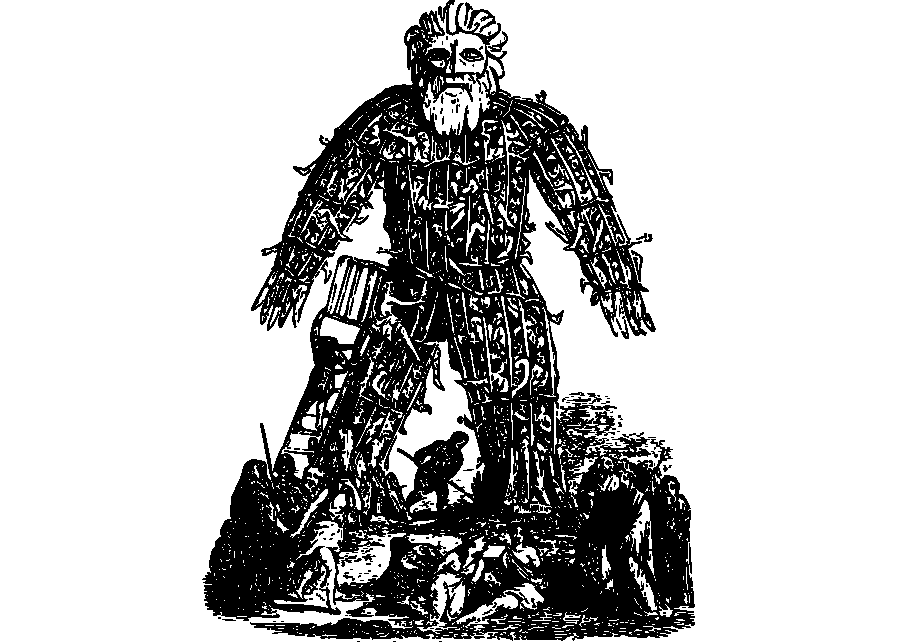
\includegraphics{./images/religion01.pdf}
\caption{Image1}
\end{figure}

In the world of role-playing games, it's important to consider the
spirituality and religious beliefs of a character. The Spirituality
Sheet is an integral part of character creation and is designed to help
players define their character's connection to the spiritual and
religious aspects of the game world. This chapter will detail the
mechanics behind the Spirituality Sheet, including the options available
for defining the strength of a character's belief or association with a
religious system, as well as any relevant traits and skills that may
impact the character's spirituality and religious beliefs. Whether
playing as a devout follower of a particular faith or a non-believer,
the Spirituality Sheet will help players bring their character to life
and create a more immersive role-playing experience.

\hypertarget{adherence}{%
\subsection{Adherence}\label{adherence}}

The ``Adherence'' field on the character sheet represents the strength
of the character's belief or association with a particular religious or
spiritual system. The options for this field range from non-believer to
orthodox adherent, providing a spectrum of beliefs that a character can
possess. The non-believer is someone who does not hold any belief in a
higher power, whereas an agnostic is someone who is uncertain about the
existence of a higher power. On the other hand, a casual adherent is
someone who holds a loose connection to their religious or spiritual
beliefs, and an orthodox adherent is someone who strictly follows the
teachings and practices of their chosen system. This mechanic helps to
further flesh out the character and their motivations, and provides a
lens through which the character may view the world around them.


\hypertarget{tolerance}{%
\subsection{Tolerance}\label{tolerance}}

This field reflects the character's willingness to accept differences of
belief in others. In determining the level of tolerance, there are three
options available for the player to choose from: Inclusive, Tolerant, or
Intolerant. The level of tolerance selected will affect how the
character interacts with people of different beliefs and religions in
the game world.

\begin{enumerate}
\def\labelenumi{\arabic{enumi}.}
\tightlist
\item
  Inclusive
\item
  Tolerant
\item
  Intolerant
\end{enumerate}

\begin{figure}
\centering
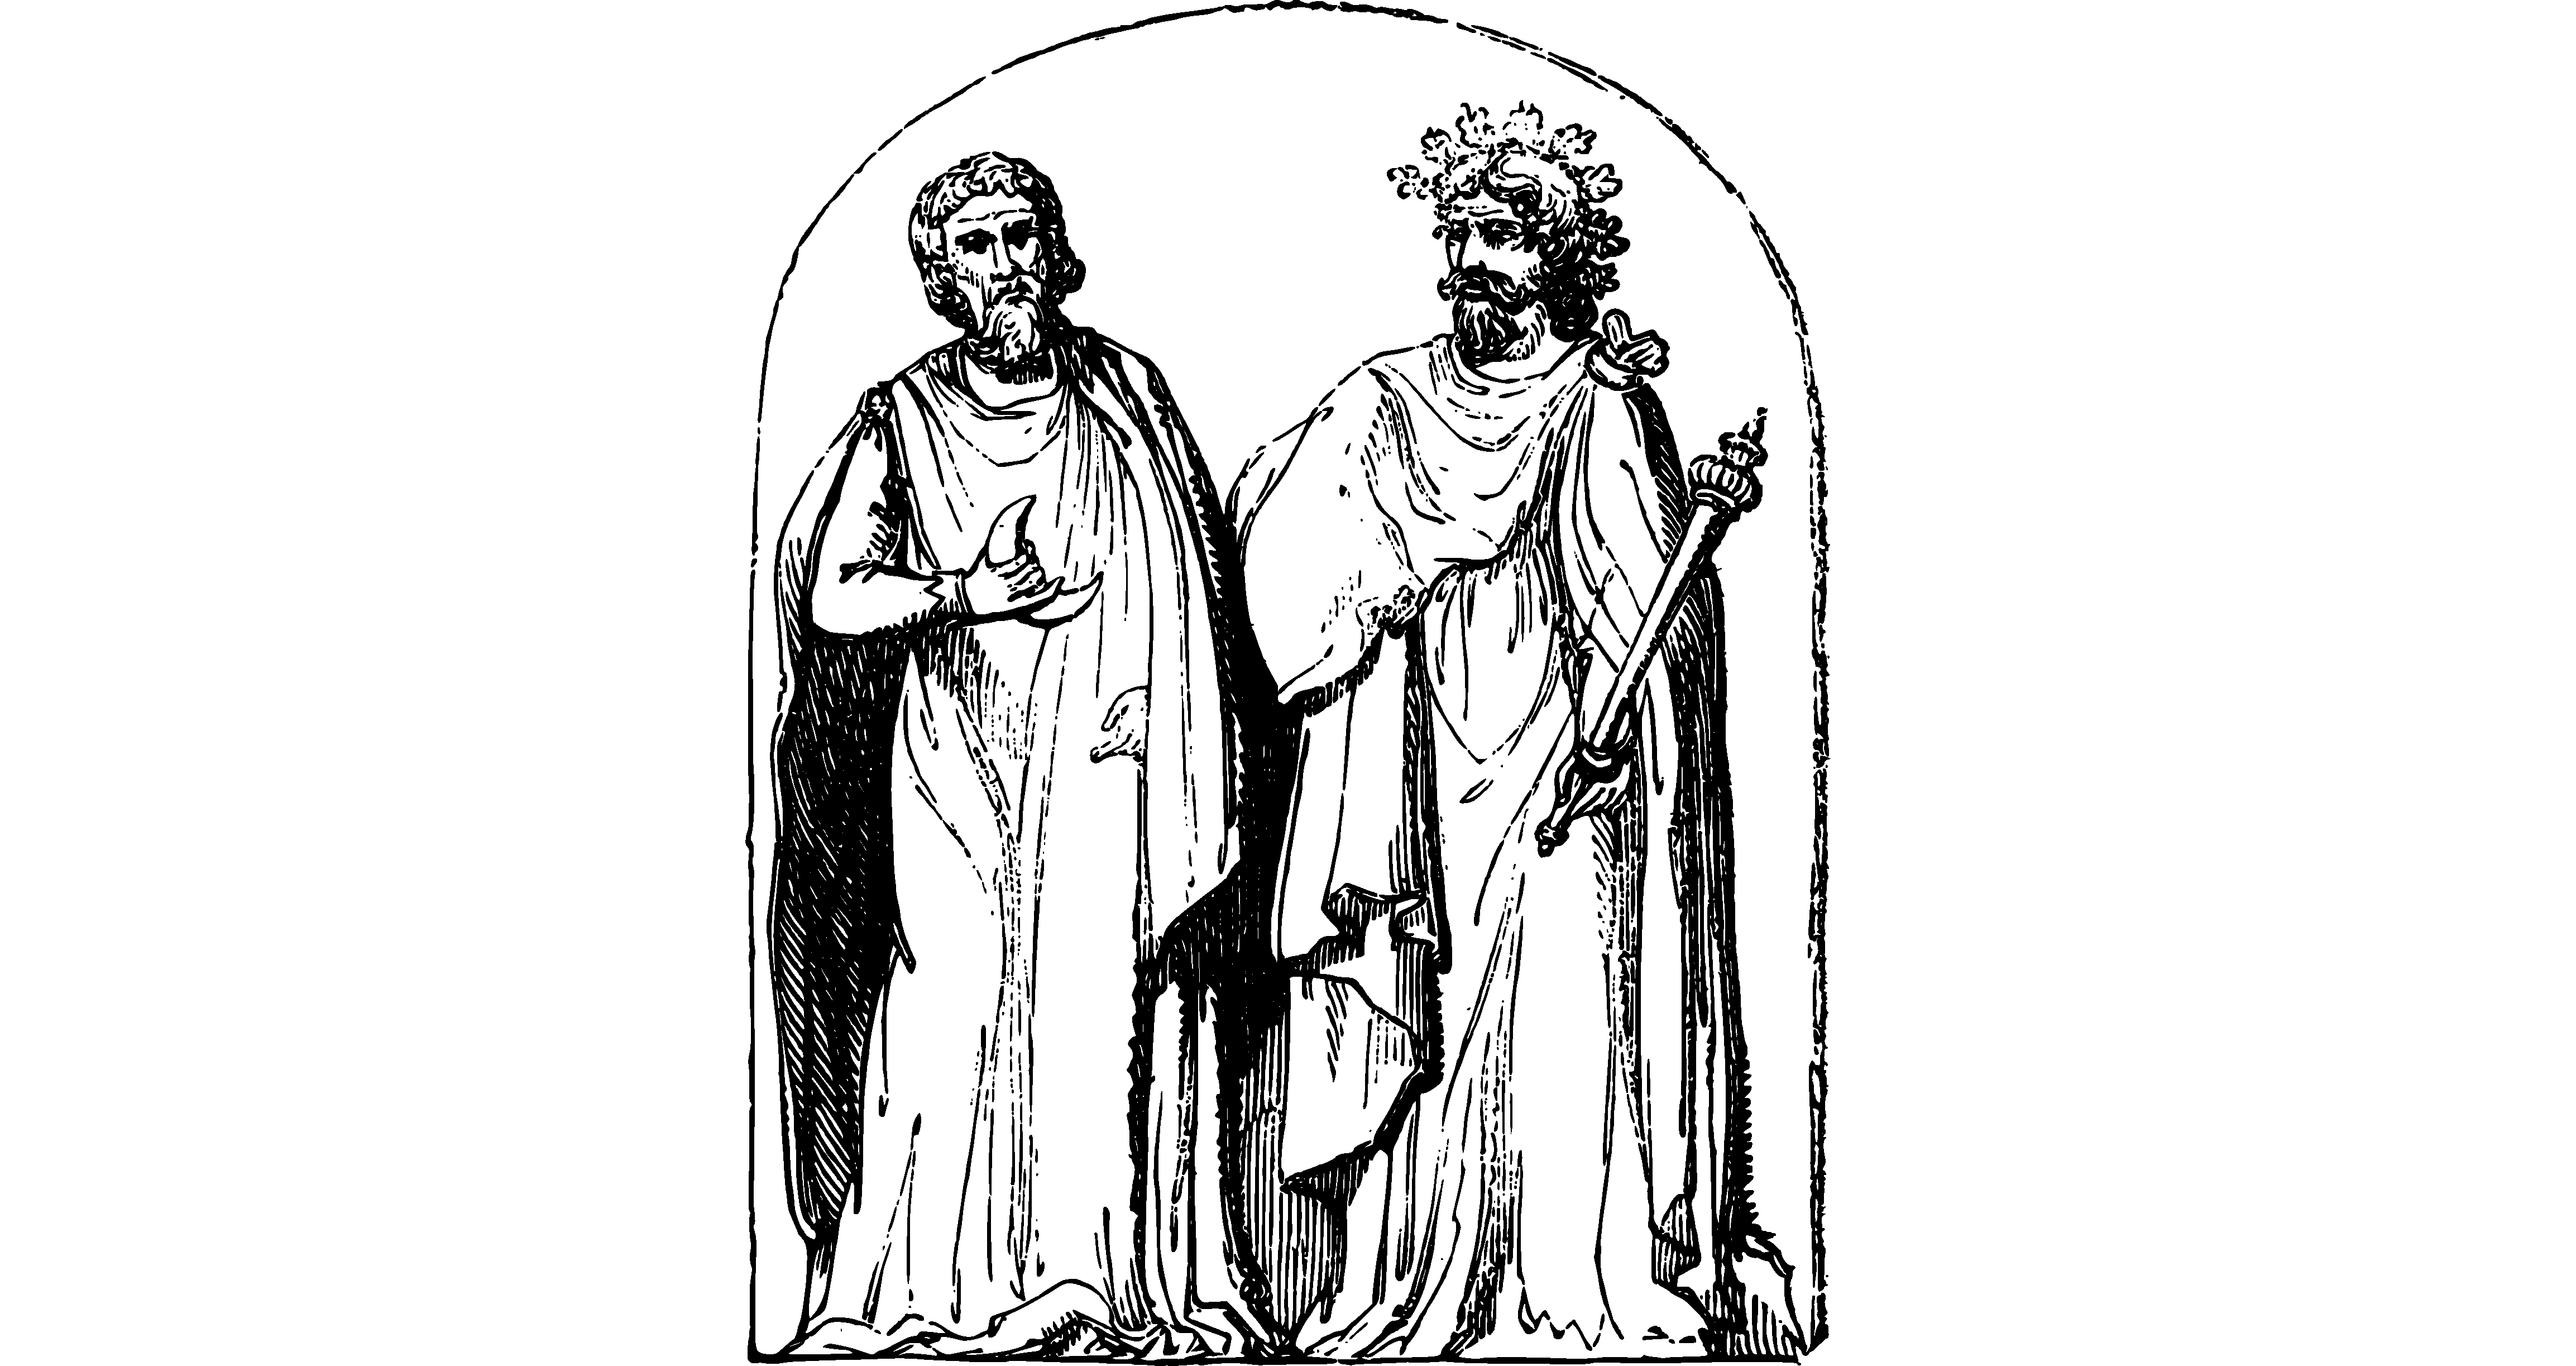
\includegraphics{./images/religion03.pdf}
\caption{Image1}
\end{figure}

\hypertarget{religious-demeanor}{%
\subsection{Religious Demeanor}\label{religious-demeanor}}

The field ``RELIGIOUS DEMEANOR'' on the character sheet aims to capture
how your character tends to act in regards to religious beliefs. To
reflect this, the player will be presented with three different fields
to fill out. The first field is ``Expression of beliefs'' and asks the
player to decide on the frequency at which their character expresses
their beliefs. The options range from ``None'', ``Occasional'', to
``Constant''. The next field is ``Converting others'', which asks the
player to choose the level of effort the character puts into converting
others to their beliefs. The choices here are ``Never'', ``Casual'', and
``Aggressive''. Finally, the ``Attitude'' field asks the player to
choose the general approach the character takes towards religion and
religious beliefs. The options for this field range from the irreverent
``Irreverent'' to the devout ``Ecstatic''. By filling out these fields,
the player can gain a deeper understanding of their character's
relationship to religion and spirituality.

\begin{longtable}[]{@{}lll@{}}
\toprule
Expression of beliefs & Converting others & Attitude \\
\midrule
\endhead
- None & - Never & - Irreverent \\
- Occasional & - Casual & - Fearful \\
- Constant & - Aggressive & - Judgmental \\
& & - Humble \\
& & - Ecstatic \\
\bottomrule
\end{longtable}

\hypertarget{religious-association}{%
\subsection{Religious association}\label{religious-association}}

The ``Religious Association'' field in the character sheet is an
important aspect of a character's spirituality. This field indicates the
character's affiliation, or lack thereof, with a religious organization
or belief system. There are a range of options available, including
Church, Cult, Fellowship, Solitary, and Indigenous, each with its own
unique meaning and characteristics.

A Church is a well-established, hierarchical religious organization,
typically with a set of beliefs and practices that are followed by its
members. A Cult is a smaller group attached to a single charismatic
leader, who may have unique or unconventional beliefs. A Fellowship is a
small, informal religious group that lacks formal organization and a
charismatic leader. Solitary is for characters who either have unique
beliefs or choose not to affiliate with others, and Indigenous refers to
religious traditions within a cultural group, such as a family or
village.

Having an understanding of a character's religious association can
provide insight into their beliefs, values, and motivations, and can
also add depth to their relationships with other characters. This field
can also play a role in the story, as it may impact the character's
actions and decisions, as well as influence how they are perceived by
others.

\begin{longtable}[]{@{}
  >{\raggedright\arraybackslash}p{(\columnwidth - 2\tabcolsep) * \real{0.0976}}
  >{\raggedright\arraybackslash}p{(\columnwidth - 2\tabcolsep) * \real{0.9024}}@{}}
\toprule
\begin{minipage}[b]{\linewidth}\raggedright
Term
\end{minipage} & \begin{minipage}[b]{\linewidth}\raggedright
Definition
\end{minipage} \\
\midrule
\endhead
Church & A large, established, and hierarchical religious organization
with a set of doctrines and practices. \\
Cult & A small or large group with a strong devotion to a single
charismatic leader, often with unconventional beliefs and practices. \\
Fellowship & A small group of like-minded individuals who gather for
religious purposes, but lack formal organization and a charismatic
leader. \\
Solitary & A character who holds unique beliefs or has chosen not to
affiliate with any religious group. \\
Indigenous & Religious traditions within a cultural group, such as a
family, village, or tribe, with a strong connection to their cultural
identity. \\
Sect & A subgroup within a larger religious organization that holds
distinct beliefs and practices. \\
Coven & A group of individuals who practice witchcraft, often with
elements of nature worship and animism. \\
Temple & A place of worship associated with a specific religion or
spiritual tradition. \\
Monastery & A religious community, often associated with a specific
order or denomination, known for their dedication to a life of
contemplation and devotion. \\
Mystic Order & A secret society or organization dedicated to the study
and practice of spiritual and esoteric knowledge. \\
\bottomrule
\end{longtable}

\begin{figure}
\centering
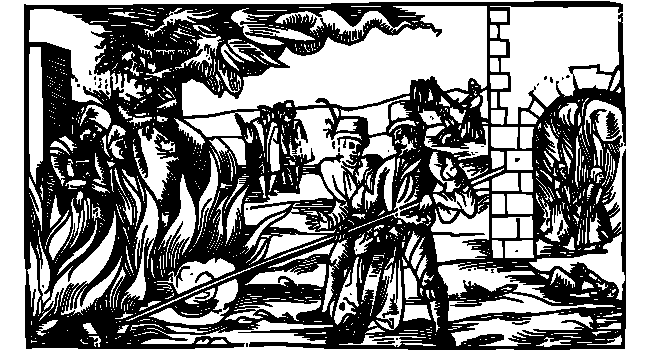
\includegraphics{./images/religion04.pdf}
\caption{Image1}
\end{figure}

\hypertarget{religious-roles}{%
\subsection{Religious Roles}\label{religious-roles}}

The ``Religious Roles'' field represents the various positions and
titles within a fictional religious organization or belief system. These
roles range from leaders and spiritual advisors, to assistants and
messengers, to protectors and mediators. Each role comes with its own
set of responsibilities and privileges, reflecting the unique aspects
and beliefs of the religion it represents. Some religious roles may be
highly respected and hold significant power within the community, while
others may be more solitary or focused on specific tasks. This field is
important for creating well-rounded and diverse religious systems within
the game world, and for providing players with the opportunity to
explore different aspects of spirituality and faith. Whether a player
chooses to play a charismatic leader or a solitary mystic, the
``Religious Roles'' field offers a wealth of opportunities for
role-playing and character development.

\begin{longtable}[]{@{}
  >{\raggedright\arraybackslash}p{(\columnwidth - 2\tabcolsep) * \real{0.1583}}
  >{\raggedright\arraybackslash}p{(\columnwidth - 2\tabcolsep) * \real{0.8417}}@{}}
\toprule
\begin{minipage}[b]{\linewidth}\raggedright
Role
\end{minipage} & \begin{minipage}[b]{\linewidth}\raggedright
Description
\end{minipage} \\
\midrule
\endhead
Abbot/Abbess & The leader of a monastery or convent. \\
Archbishop & A bishop who oversees multiple dioceses. \\
Acolyte & An assistant or beginner in religious service. \\
Bishop & An overseer of a specific area or diocese within a church. \\
Chaplain & A spiritual advisor in a specific setting, such as a hospital
or military unit. \\
Cult Leader & Usually a charismatic head of a small group of highly
devoted followers. \\
Disciple & A dedicated follower of a religious teacher or leader. \\
Elder & An experienced and respected member of a religious community. \\
Evangelist & A religious figure who spreads the gospel or message of
their faith to others. \\
Guru & A spiritual teacher. \\
Inquisitor & An official tasked with finding and ``correcting'' people
who have broken religious rules. \\
Martyr & A person who dies for their religious beliefs. \\
Missionary & Dedicated to converting others, usually in distant
geographic areas. \\
Monk/Nun & Belongs to a monastery or convent. \\
Mystic & A person who has direct experience of ultimate reality through
spiritual or mystical practices. \\
Patriarch/Matriarch & The leader of an organized religion. \\
Pilgrim & One traveling to a holy site or landmark. \\
Priest/Priestess & Someone authorized to administer sacraments as an
ordained member of a church. \\
Prophet & One inspired to utter revelations or predictions, often in
service to a deity. \\
Reverend & An honorific title given to a religious figure. \\
Sacred Courtesan & Has sex, often with strangers, in service to a
religion and for a symbolic price. \\
Mediator & A person who helps resolve conflicts and bring people
together through spiritual means. \\
Seeker & One who is searching for spiritual knowledge and
understanding. \\
Temple Guardian & A protector of a religious site, such as a temple or
shrine. \\
Wandering Monk & A roving spiritual teacher who travels from place to
place, spreading religious teachings. \\
Witch & A practitioner of magic who uses their powers for spiritual
purposes. \\
Healer & A person skilled in the use of herbs, prayers, or other methods
to cure illnesses and injuries. \\
Oracle & A person or entity that provides insight or prophesies into the
future or hidden knowledge. \\
Seer & A person who has the ability to see and understand things that
others cannot, often through spiritual means. \\
Divine Herald & A messenger of the gods, responsible for delivering
messages and performing sacred duties. \\
Sanctuary Keeper & The caretaker of a sacred place, responsible for
maintaining its sanctity and protecting it. \\
Temple Guardian & A protector of a religious site, such as a temple or
shrine. \\
Shrine Maiden & A female spiritual attendant, responsible for
maintaining the purity and sanctity of a shrine. \\
Ritualist & A person skilled in the performance of religious rituals and
ceremonies. \\
Visionary & A person who receives and interprets divine visions and
messages. \\
Soothsayer & A person who predicts future events based on astrology,
dreams, or other forms of divination. \\
Holy Knight & A warrior who serves a religious cause and protects the
faithful. \\
Chant Master & A person who leads religious music and song, often in a
religious setting. \\
Deacon & A clergy member responsible for serving the needs of a
congregation. \\
Minister & A religious leader who serves a specific denomination or
congregation. \\
Deity & A supernatural being worshipped as having power over the world
and human affairs. \\
Saint & A person recognized as holy or virtuous by a particular
religion. \\
Apostle & A messenger or disciple of a religious teacher or leader. \\
Recluse & One who lives in solitude for spiritual or religious
reasons. \\
Necromancer & A person who communicates with the dead for the purpose of
gaining knowledge or guidance. \\
\bottomrule
\end{longtable}

\begin{figure}
\centering
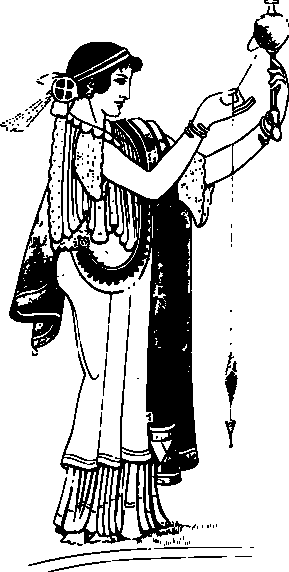
\includegraphics{./images/religion02.pdf}
\caption{Image1}
\end{figure}

\hypertarget{practicesrituals}{%
\subsection{Practices/Rituals:}\label{practicesrituals}}

The ``Practices/Rituals'' field is an important aspect of a character's
spiritual profile, as it allows players to flesh out their character's
religious beliefs and observances. This field covers the specific
rituals or practices that the character engages in, such as daily
prayers or meditations, monthly celebrations or ceremonies, seasonal
rituals, or life milestones. In addition to the type of ritual, this
field may also include information on the frequency, location, and
details of the ritual itself. For example, a character might participate
in a monthly full moon ritual that involves offering incense, reciting
prayers, and communing with their deity or spirit guide. By including
this information, players can help to create a more vivid and immersive
representation of their character's spirituality. Additionally, this
information can also be used to drive roleplaying decisions, such as the
character's reactions to certain situations or interactions with others.
Overall, the ``Practices/Rituals'' field is a valuable tool for creating
well-rounded, believable characters with unique spiritual perspectives.

\textbf{Daily prayers or meditations:}

\begin{itemize}
\tightlist
\item
  This entry would describe any daily spiritual practices the character
  engages in, such as daily prayers, meditations, or affirmations. The
  player could specify the frequency, duration, and location of these
  activities, as well as the purpose or intention behind them.
\end{itemize}

\textbf{Monthly religious celebrations or ceremonies:}

\begin{itemize}
\tightlist
\item
  This entry would describe any monthly religious events or observances
  the character participates in, such as full moon rituals, holy days,
  or feast days. The player could detail the specific celebrations or
  ceremonies, the significance or meaning behind them, and the role the
  character plays in these events.
\end{itemize}

\textbf{Seasonal rituals or observances:}

\begin{itemize}
\tightlist
\item
  This entry would describe any seasonal spiritual practices or events
  the character participates in, such as solstice or equinox ceremonies,
  harvest festivals, or other events that mark the changing of the
  seasons. The player could detail the specific rituals or observances,
  the significance or meaning behind them, and the role the character
  plays in these events.
\end{itemize}

\textbf{Life milestones or rites of passage:}

\begin{itemize}
\tightlist
\item
  This entry would describe any spiritual practices or events that mark
  important transitions or milestones in the character's life, such as
  birth, adolescence, marriage, or death. The player could detail the
  specific rituals or observances, the significance or meaning behind
  them, and the role the character plays in these events.
\end{itemize}

\textbf{Fasting or dietary restrictions:}

\begin{itemize}
\tightlist
\item
  This entry would describe any dietary restrictions or fasting
  practices the character engages in for religious or spiritual reasons.
  The player could specify the type of fasting, the frequency, and the
  reason behind it, as well as any specific dietary restrictions the
  character follows, such as vegetarianism or prohibitions against
  certain foods or ingredients.
\end{itemize}

\begin{figure}
\centering
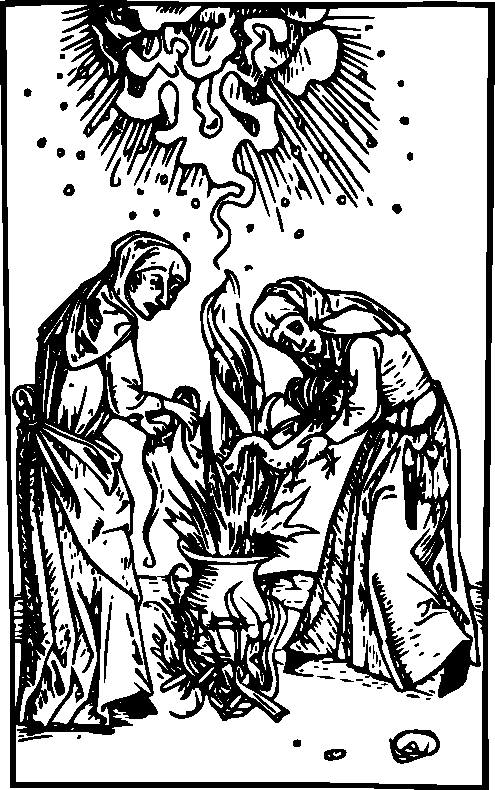
\includegraphics{./images/religion07.pdf}
\caption{Image1}
\end{figure}

\textbf{Pilgrimages or sacred journeys:}

\begin{itemize}
\tightlist
\item
  This entry would describe any pilgrimages or sacred journeys the
  character has taken or plans to take, such as visiting holy sites,
  participating in spiritual retreats, or making offerings at shrines or
  temples. The player could detail the specific destinations, the
  significance or meaning behind these journeys, and any preparations or
  rituals involved in making these trips.
\end{itemize}

\textbf{Animal or human sacrifices:}

\begin{itemize}
\tightlist
\item
  This entry would describe any instances where the character
  participates in or witnesses animal or human sacrifices as part of
  their religious or spiritual beliefs. The player could detail the
  specific reasons for these sacrifices, the religious or spiritual
  significance behind them, and any emotional or ethical conflicts the
  character experiences in relation to these practices.
\end{itemize}

\textbf{Chanting, Singing, or Dancing:}

\begin{itemize}
\tightlist
\item
  These rituals often involve repetitive vocalizations or movements that
  are meant to connect the individual with the divine or the spiritual
  realm. In some religions, singing and dancing are also used to tell
  religious stories or to give praise to a deity. These practices can be
  performed individually or as part of a group, and they can take place
  in a designated religious space or in everyday life.
\end{itemize}

\textbf{Use of Religious Symbols or Artifacts:}

\begin{itemize}
\tightlist
\item
  Religious symbols and artifacts can hold a significant spiritual
  meaning for an individual and can be used in religious practices and
  rituals. They may include objects such as crosses, statues, altars,
  prayer beads, or other items that are used to focus the individual's
  thoughts and emotions towards their religion. The use of these symbols
  and artifacts may also serve as a way to connect the individual with
  the divine, to protect themselves from harm, or to mark special
  moments in their spiritual journey.
\end{itemize}

\textbf{Spiritual or Physical Purification Rituals:}

\begin{itemize}
\tightlist
\item
  Purification rituals can take many forms and serve different purposes,
  but they typically aim to cleanse the individual of negative energies
  or influences. These rituals may involve washing or bathing, fasting,
  meditation, or the use of special incense or herbs. In some cultures,
  spiritual purification may be seen as a necessary step before engaging
  in other religious practices or before coming into contact with sacred
  spaces or objects.
\end{itemize}

\textbf{Offering of Incense or Candles:}

\begin{itemize}
\tightlist
\item
  The burning of incense or candles is a common religious practice in
  many cultures and can serve a variety of purposes. It may be used to
  create a peaceful or meditative atmosphere, to communicate with the
  divine, to make offerings to a deity, or to symbolize the individual's
  devotion. The act of lighting incense or candles may also involve
  specific rituals or prayers, making the act of offering a spiritual or
  sacred act.
\end{itemize}

\textbf{Recitation of Prayers, Mantras, or Affirmations:}

\begin{itemize}
\tightlist
\item
  The recitation of prayers, mantras, or affirmations is a common
  practice in many religions and spiritual traditions. These verbal
  expressions can serve as a way to connect with the divine, to focus
  the individual's thoughts, or to give praise or gratitude. Prayers and
  mantras may be recited individually or in a group, and they may
  involve specific actions such as bowing, kneeling, or making
  offerings.
\end{itemize}

\textbf{Meditation or Visualization Exercises:}

\begin{itemize}
\tightlist
\item
  Meditation and visualization exercises are commonly used in spiritual
  and religious contexts as a way to focus the mind and connect with the
  divine. These practices can involve focusing on a specific image or
  thought, repeating a mantra or affirmation, or simply letting the mind
  become still. Meditation and visualization can be performed in a quiet
  or sacred space, or as part of a larger ritual or ceremony.
\end{itemize}

\textbf{Communication with Gods, Spirits, or Ancestors:}

\begin{itemize}
\tightlist
\item
  Many spiritual and religious traditions involve communicating with
  gods, spirits, or ancestors as a way to seek guidance, protection, or
  to make offerings. This communication can take many forms, including
  prayer, divination, or mediumship. In some cultures, communication
  with the spiritual realm is seen as a necessary part of daily life,
  while in others it is reserved for special occasions or life events.
\end{itemize}

\textbf{Divination or prophetic rituals:}

\begin{itemize}
\tightlist
\item
  Divination or prophetic rituals involve seeking insight or knowledge
  of the future, or receiving guidance from a higher power. This could
  include practices like tarot readings, casting bones, or interpreting
  omens. These rituals are often performed by a designated individual
  within the religious community, such as a priest or shaman.
\end{itemize}

\begin{figure}
\centering
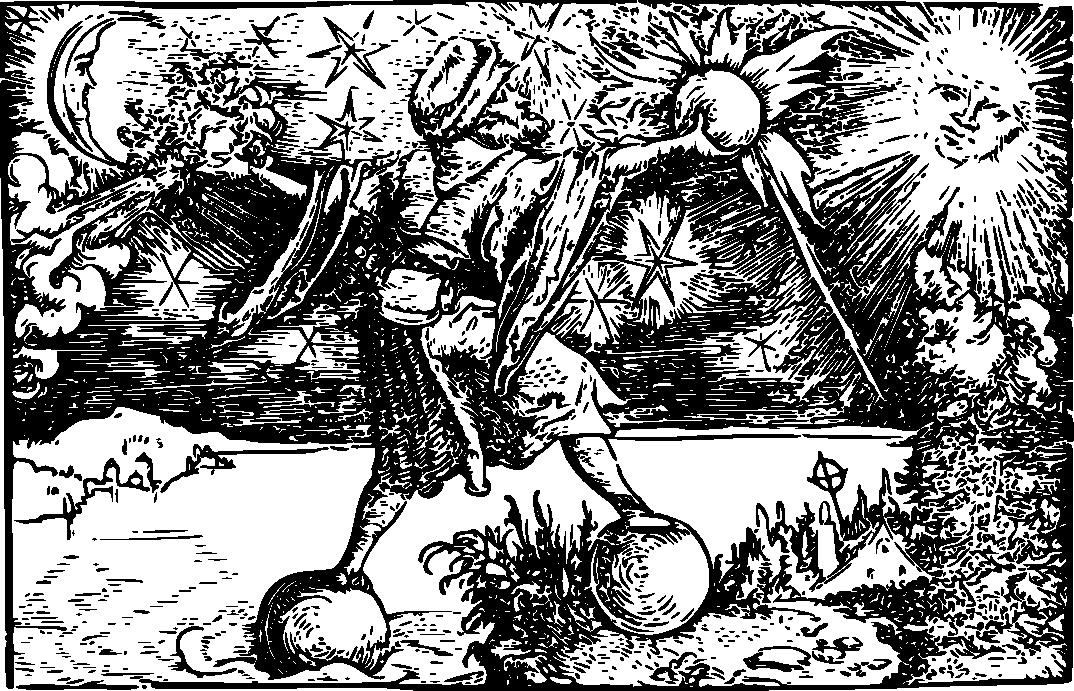
\includegraphics{./images/religion08.pdf}
\caption{Image1}
\end{figure}

\textbf{Healing or protection rituals:}

\begin{itemize}
\tightlist
\item
  Healing or protection rituals are performed with the intention of
  restoring health or providing protection to an individual or
  community. These could include practices like laying on of hands,
  reciting incantations, or using magical symbols. These rituals may be
  performed by a religious leader or by individuals seeking to heal
  themselves or others.
\end{itemize}

\textbf{Rituals involving the use of psychoactive substances:}

\begin{itemize}
\tightlist
\item
  Rituals involving the use of psychoactive substances, such as
  entheogenic plants or psychedelics, are sometimes used in religious or
  spiritual practices. These substances are believed to alter the state
  of consciousness, allowing the individual to connect with the divine
  or access higher states of awareness. These practices are often
  performed under the guidance of a shaman or spiritual leader and are
  considered sacred within some religious traditions.
\end{itemize}

\textbf{Group meditation or prayer sessions:}

\begin{itemize}
\tightlist
\item
  Group meditation or prayer sessions involve a community of individuals
  coming together to meditate, pray, or perform other spiritual
  practices in unison. These sessions are often led by a religious
  leader or facilitator and may be performed on a regular basis, such as
  daily or weekly. Group meditation or prayer sessions can provide a
  sense of community and support for those involved and can also help to
  deepen individual spiritual experiences.
\end{itemize}

\textbf{Choral performances or religious music:}

\begin{itemize}
\tightlist
\item
  Choral performances or religious music involve singing or playing
  musical instruments in a religious or spiritual context. This could
  include hymns, chants, or gospel songs. These performances may be
  performed by a choir.
\end{itemize}

\begin{figure}
\centering
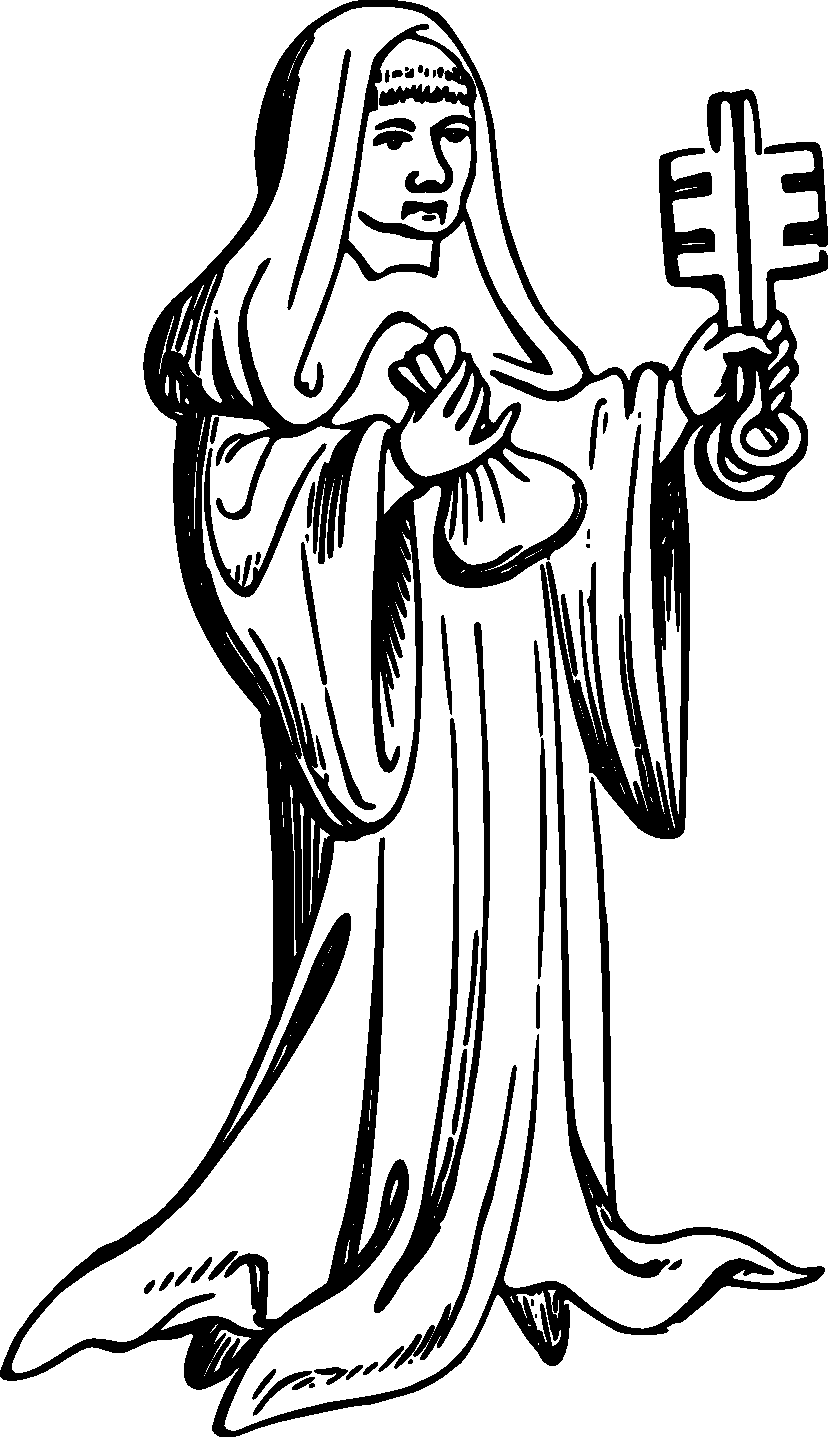
\includegraphics{./images/religion05.pdf}
\caption{Image1}
\end{figure}

\hypertarget{challenges-to-faith}{%
\subsection{Challenges to Faith}\label{challenges-to-faith}}

This field provides a platform for the player to delve into the
complexities of their character's faith and beliefs. The challenges to
faith can take various forms, each one presenting its own set of
obstacles for the character to overcome. Through detailing these trials,
the player can create a well-rounded religious background for their
character, one that reflects the multifaceted nature of faith and belief
in ancient times.

\textbf{Listed here are some examples of challenges to faith, such as:}

\begin{itemize}
\tightlist
\item
  Personal trial of faith
\item
  Encounter with a conflicting faith tradition
\item
  Questioning of core religious teachings
\item
  Uncertainty in the existence of a divine power
\item
  Loss of a cherished one who was a source of spiritual fortitude
\item
  Disagreement with a religious leader or community
\item
  Surviving a traumatic event
\item
  Exposure to alternative creeds or doctrines
\item
  Difficulty aligning religious beliefs with life experiences
\item
  Lack of satisfaction or meaning in life
\item
  Tribulation to personal morals and ethics
\item
  Negative experiences with members of a religious group
\item
  A shift in life circumstances or surroundings
\item
  Discrepancies within religious doctrine or teachings
\item
  Disillusionment with the actions of religious leaders or institutions
\item
  Inability to experience a personal spiritual connection
\item
  A change in personal values or goals
\item
  A yearning for a deeper understanding of one's beliefs
\end{itemize}

\hypertarget{conclusion-1}{%
\subsection{Conclusion}\label{conclusion-1}}

In conclusion, the Spirituality Sheet provides a comprehensive way to
shape a character's religious and spiritual beliefs within the game
world. By exploring the various aspects of adherence, tolerance,
religious demeanor, association, roles, practices and rituals, as well
as challenges to faith, players can craft a well-rounded and believable
character that is truly reflective of their personal beliefs and
experiences. The Spirituality Sheet is a valuable tool for bringing
depth and dimension to a character and allowing players to fully immerse
themselves in their role-playing experience. Whether your character is
devout, questioning, or somewhere in between, the Spirituality Sheet
provides the framework necessary to create a truly authentic and
engaging character.

\begin{figure}
\centering
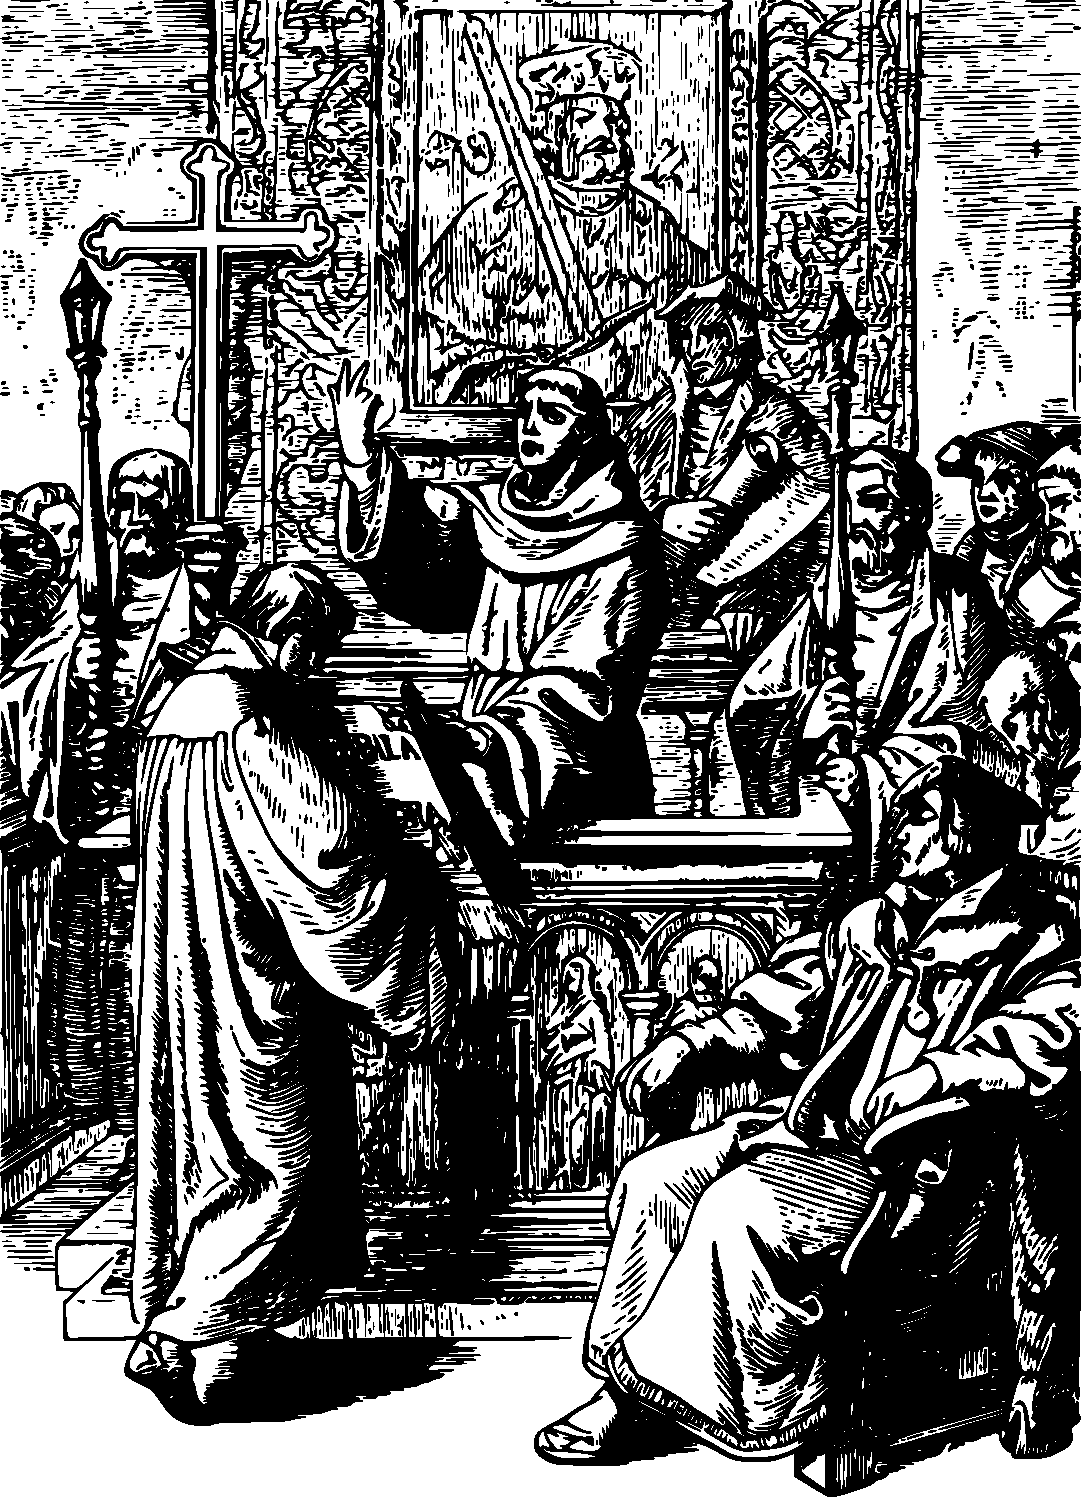
\includegraphics{./images/religion06.pdf}
\caption{Image1}
\end{figure}

\hypertarget{physical-description}{%
\section{Physical Description}\label{physical-description}}

This chapter delves into the intricate details that bring characters to
life within the world of Eidos. As players embark on their imaginative
journeys, this section serves as a guide to creating vivid and visually
appealing characters. A character's physical appearance not only shapes
their identity but also influences how they interact with the game's
immersive setting.

Within this chapter, players will discover a wealth of options and
considerations to craft the perfect physical representation of their
character. From facial features and body types to hairstyles and
clothing choices, each element contributes to a unique and memorable
persona. Whether it's a towering warrior with a battle-scarred face, a
nimble rogue with piercing eyes, or a mystical spellcaster adorned in
intricate robes, the physical description chapter empowers players to
manifest their characters' appearances with precision and creativity.

By providing a comprehensive exploration of physical traits, this
chapter ensures that every player has the tools necessary to design
characters that not only reflect their imagination but also contribute
to the depth and immersion of the game world. With attention to detail
and an emphasis on personal expression, Eidos encourages players to
embrace their creativity and bring forth characters that will leave a
lasting impression on their adventures.

\hypertarget{body}{%
\subsection{Body}\label{body}}

The human form is a canvas for storytelling, and body types play a
significant role in shaping a character's physical presence. In this
section, we delve into the diverse aspects of body types, starting with
\textbf{Height}. Explore how height can influence perception, power
dynamics, and interactions within your character's world.

\begin{longtable}[]{@{}l@{}}
\toprule
Height Options \\
\midrule
\endhead
Tall \\
Average \\
Short \\
Very Tall \\
Very Short \\
\bottomrule
\end{longtable}

Next, we examine the concept of \textbf{Build}, exploring different body
shapes and sizes and their impact on character traits and capabilities.

\begin{longtable}[]{@{}l@{}}
\toprule
Build Options \\
\midrule
\endhead
Slender and Athletic \\
Robust and Heavily Built \\
Lean and Muscular \\
Petite and Delicate \\
\bottomrule
\end{longtable}

Finally, we discuss the importance of \textbf{Proportions}, highlighting
how well-balanced proportions contribute to a visually appealing and
believable character.

\begin{longtable}[]{@{}l@{}}
\toprule
Proportions Options \\
\midrule
\endhead
Well-Balanced \\
Long Limbs \\
Short Torso \\
Broad Shoulders \\
Proportionate Limbs \\
\bottomrule
\end{longtable}

Consider the expanded options for each aspect to further customize your
character's height, build, and proportions. These choices will help
shape your character's physical presence, traits, and visual identity
within the game world.

\hypertarget{skin-and-skintone}{%
\subsection{Skin and Skintone}\label{skin-and-skintone}}

The skin is the outermost layer of the body, providing protection and
serving as a canvas for expression. In this section, we explore the
intricate aspects of skin and skintone, allowing you to create
characters with diverse appearances and backgrounds.

\textbf{Skin Texture}

Skin texture refers to the surface quality and appearance of the skin.
It can vary from smooth and flawless to rough and weathered, adding
depth and realism to your character's visual representation. Consider
the following options for skin texture:

\begin{longtable}[]{@{}
  >{\raggedright\arraybackslash}p{(\columnwidth - 2\tabcolsep) * \real{0.0584}}
  >{\raggedright\arraybackslash}p{(\columnwidth - 2\tabcolsep) * \real{0.9416}}@{}}
\toprule
\begin{minipage}[b]{\linewidth}\raggedright
Texture
\end{minipage} & \begin{minipage}[b]{\linewidth}\raggedright
Description
\end{minipage} \\
\midrule
\endhead
Smooth & Skin with a smooth and even texture, free from visible
blemishes, scars, or imperfections. It appears soft, supple, and
well-nourished. \\
Freckled & Skin with scattered freckles across the face and sometimes
other areas of the body. Freckles are small, pigmented spots that add
charm and youth. \\
Wrinkled & Skin with visible wrinkles and fine lines, often associated
with aging or exposure to environmental factors. It appears creased or
folded. \\
Blemished & Skin with noticeable blemishes such as acne, pimples, or
blackheads. It may appear inflamed or uneven in texture. \\
Dimpled & Skin with small, natural indentations known as dimples, often
seen on cheeks or chin. Dimples can add a touch of charm and
playfulness. \\
Weathered & Skin that shows signs of exposure to harsh elements, such as
wind or sun damage. It may appear rough, dry, or aged. \\
Glowing & Skin that radiates a healthy glow and appears vibrant, often
associated with good health and a balanced lifestyle. \\
\bottomrule
\end{longtable}

By selecting a specific skin texture, you can visually convey your
character's history, lifestyle, and unique traits, enhancing their depth
and storytelling potential.

\textbf{Skintone}

Skintone encompasses the coloration of the skin, which can vary across a
broad spectrum. It is influenced by factors such as genetics,
environment, and cultural heritage. Explore the diverse skintone options
for your character:

\begin{longtable}[]{@{}
  >{\raggedright\arraybackslash}p{(\columnwidth - 2\tabcolsep) * \real{0.0649}}
  >{\raggedright\arraybackslash}p{(\columnwidth - 2\tabcolsep) * \real{0.9351}}@{}}
\toprule
\begin{minipage}[b]{\linewidth}\raggedright
Skintone
\end{minipage} & \begin{minipage}[b]{\linewidth}\raggedright
Description and Visual Comparison
\end{minipage} \\
\midrule
\endhead
Fair & A light complexion with a delicate, porcelain-like appearance.
Similar to fresh snow or fine china. \\
Light & A pale and subtle skintone with a soft and gentle complexion.
Similar to a petal or light cream. \\
Pale & A very light skintone with minimal color and a delicate
complexion. Similar to a pearl or light mist. \\
Porcelain & A smooth and pale skintone resembling fine porcelain or
alabaster. Similar to fine porcelain or marble. \\
Ivory & A creamy and pale skintone with a soft, warm undertone. Similar
to ivory or warm sand. \\
Beige & A warm and neutral skintone with a light tan hue. Similar to
beige or light caramel. \\
Natural & A balanced and neutral skintone resembling the natural color
of human skin. Similar to natural skin color or sand. \\
Golden & A warm skintone with a subtle golden hue, giving a radiant and
sun-kissed appearance. Similar to golden wheat or honey. \\
Peach & A soft and warm skintone with a gentle peachy undertone. Similar
to a ripe peach or apricot. \\
Rosy & A skintone with a rosy or pinkish hue, giving a healthy and
youthful appearance. Similar to a rose petal or flushed cheeks. \\
Warm & A warm-toned skintone with a sun-kissed appearance and golden
undertones. Similar to warm sand or sunlit bronze. \\
Olive & A skintone with a greenish or yellowish undertone, often found
in individuals with Mediterranean heritage. Similar to olive skin or
light khaki. \\
Tawny & A warm and tan skintone with a mix of golden and brown
undertones. Similar to tawny leather or caramel. \\
Caramel & A rich and warm skintone resembling the color of caramel or
toffee. Similar to caramel or warm toffee. \\
Honey & A warm and golden skintone with rich undertones, resembling the
color of honey. Similar to honey or amber. \\
Bronze & A deep and warm skintone with a bronze-like appearance. Similar
to a bronze sculpture or copper. \\
Tan & A medium to dark skintone with a warm and sun-kissed appearance.
Similar to tanned skin or rich sand. \\
Amber & A deep and warm skintone with a reddish or amber-like hue.
Similar to amber or burnt sienna. \\
Sunkissed & A warm skintone with a sun-kissed appearance, often achieved
from spending time in the sun. Similar to a sun-kissed glow or bronzed
skin. \\
Brown & A medium to dark skintone with brown hues and warm undertones.
Similar to rich brown or dark chocolate. \\
Cocoa & A deep and rich skintone resembling the color of cocoa or dark
chocolate. Similar to cocoa or dark chocolate. \\
Mahogany & A dark and warm skintone with deep reddish-brown hues.
Similar to mahogany wood or chestnut. \\
Chestnut & A deep and warm skintone resembling the color of chestnuts.
Similar to chestnuts or deep earth tones. \\
Mocha & A dark and rich skintone with a mix of brown and warm
undertones. Similar to a mocha coffee or dark wood. \\
Dark & A deep and dark skintone with rich, dark brown hues. Similar to
deep ebony or dark soil. \\
Ebony & A very dark and intense skintone, often found in individuals
with African heritage. Similar to ebony wood or black velvet. \\
Deep Brown & A deep and rich brown skintone with dark undertones.
Similar to deep brown or dark chocolate. \\
Coffee & A deep and rich skintone resembling the color of coffee beans.
Similar to coffee beans or dark bark. \\
Onyx & A pitch-black skintone with no discernible undertones. Similar to
onyx or black velvet. \\
\bottomrule
\end{longtable}

Choosing a skintone helps define your character's ethnicity, ancestry,
and cultural identity. It adds richness and authenticity to their visual
portrayal, further immersing players into the world of your RPG.

\textbf{Complexion}

Complexion refers to the overall appearance and condition of the skin,
including factors such as brightness, clarity, and health. It can range
from a radiant and flawless complexion to a more sallow or troubled one.
Consider the following complexion options:

\begin{longtable}[]{@{}
  >{\raggedright\arraybackslash}p{(\columnwidth - 2\tabcolsep) * \real{0.0645}}
  >{\raggedright\arraybackslash}p{(\columnwidth - 2\tabcolsep) * \real{0.9355}}@{}}
\toprule
\begin{minipage}[b]{\linewidth}\raggedright
Complexion
\end{minipage} & \begin{minipage}[b]{\linewidth}\raggedright
Description
\end{minipage} \\
\midrule
\endhead
Radiant & A complexion that appears glowing, healthy, and vibrant. The
skin has a natural radiance, often associated with good health and
vitality. \\
Clear & A complexion that is smooth, even, and free from blemishes or
imperfections. The skin appears flawless and has a naturally clear and
bright tone. \\
Ruddy & A complexion that has a reddish or rosy undertone, often
associated with a healthy flush. The skin appears lively, with a natural
rosy hue. \\
Sallow & A complexion that has a yellowish or pale undertone, often
associated with fatigue or illness. The skin appears dull or lacking in
vitality. \\
Acne-Prone & A complexion that is prone to acne breakouts or blemishes.
The skin may have visible pimples, redness, or inflammation due to acne
or oily skin. \\
\bottomrule
\end{longtable}

By selecting a specific complexion, you can add another layer of detail
to your character, highlighting their physical well-being, lifestyle, or
even their struggles.

Create characters with unique skin textures, skintones, and complexions
to represent a wide range of backgrounds, ethnicities, and experiences.
The choices you make in this aspect of character creation contribute to
their visual identity and help shape their story within the game world.

\hypertarget{eyes}{%
\subsection{Eyes}\label{eyes}}

The face is a canvas that reveals the uniqueness and character of a
person. In this section, we delve into the intricacies of facial
features, exploring the mesmerizing world of eyes, the windows to the
soul. Discover how the shape, color, and expression of the eyes can add
depth and personality to your character.

** Eye Colors **

\begin{longtable}[]{@{}
  >{\raggedright\arraybackslash}p{(\columnwidth - 2\tabcolsep) * \real{0.0350}}
  >{\raggedright\arraybackslash}p{(\columnwidth - 2\tabcolsep) * \real{0.9650}}@{}}
\toprule
\begin{minipage}[b]{\linewidth}\raggedright
Color
\end{minipage} & \begin{minipage}[b]{\linewidth}\raggedright
Description
\end{minipage} \\
\midrule
\endhead
Brown & A warm, earthy color resembling the rich tones of coffee beans,
chestnuts, or fertile soil. It can range from light caramel to deep
chocolate, mirroring the shades found in the bark of trees or the
feathers of certain birds. \\
Blue & Reminiscent of a clear sky or the shimmering surface of a calm
lake, blue eyes vary from a pale, icy blue to a vibrant sapphire or deep
indigo. They can evoke images of serene waters, delicate flowers like
forget-me-nots, or the wings of certain butterflies. \\
Green & Reflecting the lushness of the natural world, green eyes can
range from a vibrant emerald to a soft, mossy green. They resemble the
color of fresh grass, leaves in a dense forest, or the captivating
iridescence of certain gemstones like jade or malachite. \\
Hazel & A captivating mix of colors, hazel eyes showcase various hues
such as warm browns, soft greens, and hints of gold. They can resemble
the vibrant shades seen in autumn leaves, a cup of creamy hazelnut
coffee, or the dappled patterns on the wings of butterflies or birds. \\
Gray & Exhibiting a cool and subtle tone, gray eyes can resemble the
color of storm clouds, morning mist, or the feathers of certain birds
like pigeons or doves. They can also have a silvery sheen, reminiscent
of moonlit nights or the reflective surface of a calm lake. \\
Amber & Radiating a warm, golden color, amber eyes resemble the glowing
embers of a cozy fire or the rich hues of autumn leaves basking in
sunlight. They can bring to mind the warm glow of a candle or the golden
strands of honey dripping from a spoon. \\
Violet & A mesmerizing purple color reminiscent of delicate lavender
fields, royal amethyst gemstones, or the petals of enchanting flowers
like violets or orchids. Violet eyes can evoke a sense of mystery,
magic, and ethereal beauty. \\
Black & Deep and intense, black eyes are as dark as a moonless night.
They can resemble the glossy feathers of certain birds, the obsidian
surface of volcanic rock, or the captivating darkness of a starless
sky. \\
Red & Unusual and captivating, red eyes possess a vibrant crimson hue
that can resemble the fiery glow of molten lava, the intensity of a
blazing fire, or the striking color of a red rose in full bloom. They
convey a sense of passion, intensity, or otherworldly allure. \\
Violet-Blue & A captivating fusion of violet and blue, violet-blue eyes
exhibit a mesmerizing shade reminiscent of a twilight sky. They can
resemble the hues seen during a breathtaking sunset, the delicate petals
of blue violets, or the radiant colors found in certain gemstones like
tanzanite. \\
Gray-Blue & A subtle blend of gray and blue, gray-blue eyes have a cool
and calming appearance. They can bring to mind the colors of a misty
morning sky, the soft reflection on a calm lake, or the delicate
patterns on seashells washed ashore. \\
Green-Hazel & Combining the beauty of green and hazel, green-hazel eyes
showcase a captivating mix of warm greens, golden browns, and hints of
amber. They can resemble the lush tones found in a sun-dappled forest,
the intricate patterns on a butterfly's wings, or the vibrant colors of
certain gemstones like peridot. \\
Gold & Resembling the precious metal it is named after, gold eyes
possess a radiant and luminous hue. They can evoke images of the golden
rays of the sun, the shimmering surface of a calm lake reflecting
sunlight, or the warm glow of a candle flame. \\
Silver & Exhibiting a cool and striking appearance, silver eyes have a
silvery-gray or bluish-gray hue reminiscent of moonlit nights,
shimmering frost, or the reflective surface of a calm lake. They convey
a sense of grace, wisdom, and a touch of enchantment. \\
Turquoise & A vibrant and captivating color reminiscent of the gemstone
it is named after, turquoise eyes showcase a mix of blue and green
tones. They can resemble the hues found in tropical waters, the
iridescent feathers of certain birds like peacocks, or the mesmerizing
colors of a coral reef. \\
Topaz & Resembling the warm, golden-brown tones of the gemstone, topaz
eyes radiate a captivating charm. They can evoke images of the sun's
golden rays, the rich colors of a harvest field, or the luminous glow of
a bonfire on a cool evening. \\
Sapphire & Like the deep blue gemstone it is named after, sapphire eyes
possess a rich and captivating blue hue. They evoke a sense of depth,
allure, and a touch of sophistication, akin to the depths of the ocean
or the clarity of a pristine waterfall. \\
Emerald & Radiating a lush and vibrant green color, emerald eyes capture
attention and convey a sense of vitality, growth, and natural elegance.
They can resemble the verdant shades of emerald gemstones, the vibrant
foliage of a tropical rainforest, or the glimmering surface of a
tranquil pond. \\
Amethyst & A captivating purple color reminiscent of the gemstone it
shares its name with, amethyst eyes possess a rich, violet-purple hue.
They exude an air of mystery, enchantment, and a touch of royalty. They
can bring to mind the deep hues of amethyst crystals or the delicate
petals of lavender flowers. \\
\bottomrule
\end{longtable}

** Eye Shapes **

\begin{longtable}[]{@{}
  >{\raggedright\arraybackslash}p{(\columnwidth - 2\tabcolsep) * \real{0.0990}}
  >{\raggedright\arraybackslash}p{(\columnwidth - 2\tabcolsep) * \real{0.9010}}@{}}
\toprule
\begin{minipage}[b]{\linewidth}\raggedright
Shape
\end{minipage} & \begin{minipage}[b]{\linewidth}\raggedright
Description
\end{minipage} \\
\midrule
\endhead
Round & The most common shape, often associated with innocence and
openness. \\
Almond & A graceful and elongated shape, often symbolizing elegance and
sensuality. \\
Hooded & Characterized by a heavy upper lid, conveying a sense of
mystery and secrecy. \\
Deep-Set & Set deeply into the sockets, creating an intense and soulful
appearance. \\
Wide-Set & Positioned farther apart, suggesting a more open and friendly
expression. \\
Upturned & Featuring an upward tilt at the outer corners, expressing a
playful and mischievous nature. \\
Downturned & Sloping downwards at the outer corners, reflecting a hint
of sadness or weariness. \\
Monolid & Smooth, without a visible crease, common in East Asian and
Southeast Asian cultures. \\
Protruding & Extending outward from the face, often associated with an
intense and observant gaze. \\
\bottomrule
\end{longtable}

** Eye Sizes **

When considering eye sizes, it's important to note that there is a wide
range of natural variation. The size of the eyes can contribute to the
overall appearance and expression of a character. Here are some common
descriptors:

\begin{itemize}
\tightlist
\item
  \textbf{Large:} Expressive, captivating, and often associated with
  innocence or a childlike quality.
\item
  \textbf{Small:} Intense, focused, and can convey a sense of mystery or
  intensity.
\item
  \textbf{Average:} Balanced and versatile, suitable for a wide range of
  character types.
\item
  \textbf{Uneven:} Different-sized eyes can add a unique and intriguing
  element to a character's appearance, highlighting their individuality.
\end{itemize}

** Eyelashes **

\begin{longtable}[]{@{}
  >{\raggedright\arraybackslash}p{(\columnwidth - 2\tabcolsep) * \real{0.0654}}
  >{\raggedright\arraybackslash}p{(\columnwidth - 2\tabcolsep) * \real{0.9346}}@{}}
\toprule
\begin{minipage}[b]{\linewidth}\raggedright
Eyelash
\end{minipage} & \begin{minipage}[b]{\linewidth}\raggedright
Description
\end{minipage} \\
\midrule
\endhead
Long & Dramatic and attention-grabbing lashes that enhance the
character's gaze. \\
Thick & Dense and voluminous lashes that give a fuller appearance to the
eyes. \\
Curled & Lashes that are naturally curled or enhanced with curlers,
creating an expressive and alluring look. \\
Sparse & Thin or sparsely distributed lashes that can convey subtlety,
vulnerability, or a delicate beauty. \\
Natural & Unadorned lashes that appear as they are, emphasizing a
natural and effortless beauty. \\
\bottomrule
\end{longtable}

** Eyebrows **

\begin{longtable}[]{@{}
  >{\raggedright\arraybackslash}p{(\columnwidth - 2\tabcolsep) * \real{0.1444}}
  >{\raggedright\arraybackslash}p{(\columnwidth - 2\tabcolsep) * \real{0.8556}}@{}}
\toprule
\begin{minipage}[b]{\linewidth}\raggedright
Eyebrow Shape
\end{minipage} & \begin{minipage}[b]{\linewidth}\raggedright
Description
\end{minipage} \\
\midrule
\endhead
Arched & Graceful curves that add elegance and intensity to the eyes. \\
Straight & Horizontal brows that give a calm and balanced appearance. \\
Thin & Delicate and slender brows that can evoke a sense of refinement
or fragility. \\
Thick & Full and prominent brows that convey strength and boldness. \\
Angular & Sharply defined angles that create a striking and expressive
look. \\
\bottomrule
\end{longtable}

\hypertarget{nose}{%
\subsection{Nose}\label{nose}}

Among the distinguishing features of the face, the nose holds a
significant role in defining a character's appearance. In this section,
we explore the various shapes, sizes, and nuances of noses, uncovering
how this subtle yet prominent feature can contribute to the overall
characterization of your creation.

\textbf{Nose Shapes}

When creating a character, the choice of nose shape holds great
importance in defining their appearance and personality. The selected
nose shape adds depth and nuance to the character's visual portrayal,
contributing to their overall characterization. Whether it's a straight
nose, conveying a sense of balance and refinement, or a Roman nose,
symbolizing strength and authority, each shape helps players envision
their character's traits and role in the game world. By choosing a
specific nose shape, players can bring their characters to life,
aligning their physical features with their desired persona and
enhancing the immersive experience of character creation.

\begin{longtable}[]{@{}
  >{\raggedright\arraybackslash}p{(\columnwidth - 2\tabcolsep) * \real{0.0386}}
  >{\raggedright\arraybackslash}p{(\columnwidth - 2\tabcolsep) * \real{0.9614}}@{}}
\toprule
\begin{minipage}[b]{\linewidth}\raggedright
Shape
\end{minipage} & \begin{minipage}[b]{\linewidth}\raggedright
Description
\end{minipage} \\
\midrule
\endhead
Straight & A nose with a straight bridge, often associated with elegance
and symmetry. It portrays a sense of balance and can contribute to a
refined and classic appearance. \\
Roman & Also known as an aquiline nose, it has a prominent bridge with a
slight downward curve. This shape can evoke a sense of strength,
authority, and nobility. \\
Button & Characterized by a small, rounded tip, the button nose exudes a
charming and youthful appeal. It is often associated with cuteness,
innocence, and a playful demeanor. \\
Upturned & With a slightly upturned tip, this nose shape creates an
appearance of perkiness and whimsy. It can add a touch of quirkiness or
mischievousness to a character's countenance. \\
Snub & The snub nose features a short and slightly upturned tip, often
coupled with a slightly concave bridge. It can convey a sense of charm,
impishness, or a hint of rebelliousness. \\
Greek & Resembling the sculptures of ancient Greek gods, this nose shape
has a straight bridge and a narrow, well-defined tip. It exudes an aura
of elegance, grace, and timeless beauty. \\
Hawk & Similar to the beak of a hawk, this nose shape has a prominent,
curved bridge with a sharp downward angle. It can portray an assertive,
confident, and strong-willed character. \\
Snorkel & Unconventional and unique, the snorkel nose has an extended
and protruding shape resembling a snorkel tube. It adds a distinctive
and eccentric touch to a character's appearance. \\
Crooked & Characterized by a noticeable deviation from a straight line,
the crooked nose exhibits an asymmetrical shape. It can suggest a
rugged, unconventional, or mysterious persona. \\
Flat & Featuring a minimal bridge height, the flat nose has a broad and
low profile. It is often associated with certain ethnicities and can
convey a sense of heritage, cultural identity, or natural beauty. \\
\bottomrule
\end{longtable}

\textbf{Nose Sizes}

In character creation, the size of the nose plays a significant role in
shaping the character's visual identity. The chosen nose size can convey
various attributes and characteristics, influencing how the character is
perceived by others. A small nose may suggest delicacy, grace, or
subtlety, while a large nose can imply strength, resilience, or even
dominance. Players have the opportunity to carefully consider the impact
of their character's nose size, ensuring it aligns with their envisioned
persona and adds depth to their character's visual representation.

\begin{longtable}[]{@{}
  >{\raggedright\arraybackslash}p{(\columnwidth - 2\tabcolsep) * \real{0.0330}}
  >{\raggedright\arraybackslash}p{(\columnwidth - 2\tabcolsep) * \real{0.9670}}@{}}
\toprule
\begin{minipage}[b]{\linewidth}\raggedright
Size
\end{minipage} & \begin{minipage}[b]{\linewidth}\raggedright
Description
\end{minipage} \\
\midrule
\endhead
Small & A small nose is delicate and petite in proportion to the face.
It can convey a sense of gracefulness, refinement, or youthful
innocence. \\
Medium & A medium-sized nose is considered average in proportion to the
face. It is versatile and can complement various facial features,
providing a balanced and harmonious appearance. \\
Large & A large nose is more prominent and commanding, drawing attention
to the center of the face. It can suggest strength, character, and
individuality. \\
Long & A long nose extends vertically, with a noticeable length between
the bridge and the tip. It can add an elegant and regal touch to a
character's countenance. \\
Short & A short nose is characterized by its reduced length, creating a
compact and concise appearance. It can contribute to a youthful or cute
expression. \\
\bottomrule
\end{longtable}

\textbf{Nose Nuances}

The unique features of a character's nose are important elements in the
character creation process. From the presence of a bridge bump or a
nasal ridge to the absence of any pronounced features, these details
contribute to the character's overall appearance and storytelling
potential. A bridge bump can imply ruggedness or a history of battles
fought, while a nasal ridge might signify a strong and resolute
character. Conversely, a lack of notable features can add an air of
simplicity or mystery to the character. By incorporating these nose
features into the character creation process, players can further
customize their characters, adding depth and uniqueness to their
narrative experiences.

\begin{longtable}[]{@{}
  >{\raggedright\arraybackslash}p{(\columnwidth - 2\tabcolsep) * \real{0.0684}}
  >{\raggedright\arraybackslash}p{(\columnwidth - 2\tabcolsep) * \real{0.9316}}@{}}
\toprule
\begin{minipage}[b]{\linewidth}\raggedright
Nuance
\end{minipage} & \begin{minipage}[b]{\linewidth}\raggedright
Description
\end{minipage} \\
\midrule
\endhead
Rounded & A rounded nose has soft, curved contours, giving a gentle and
approachable impression. It can convey warmth, friendliness, and a
nurturing nature. \\
Angular & An angular nose has sharp and well-defined features, with
distinct lines and angles. It can suggest strength, determination, and a
more assertive personality. \\
Tapered & A tapered nose gradually narrows towards the tip, creating a
sleek and refined appearance. It can add a touch of elegance and
sophistication to a character's face. \\
Broad & A broad nose has a wider shape, often with a more substantial
base. It can convey a sense of strength, vitality, and resilience. \\
Pointed & A pointed nose features a defined and sharp tip, adding a
distinctive and slightly exotic element to a character's facial
structure. It can evoke a sense of intrigue and allure. \\
Upward-Turned & With an upward turn at the tip, this nose nuance creates
a cheerful and optimistic expression. It can contribute to a character's
cheerful, lively, or mischievous demeanor. \\
Downturned & A downturned nose has a slight droop at the tip, creating a
subtle melancholic or pensive look. It can suggest a reflective,
introspective, or more serious disposition. \\
Upward-Bridge & This nuance describes a nose with an elevated bridge,
adding a distinctive feature to a character's facial structure. It can
create a regal, refined, or statuesque appearance. \\
Flat-Bridge & A flat bridge indicates a nose with a minimal or flattened
nasal bridge. It can be associated with certain ethnicities or convey a
unique and unconventional character. \\
\bottomrule
\end{longtable}

\hypertarget{mouth}{%
\subsection{Mouth}\label{mouth}}

The mouth is a gateway to expression, communication, and emotion. It is
a focal point of the face that can greatly influence the portrayal of a
character. In this section, we delve into the captivating aspects of the
mouth, including the shape of the lips, the positioning of the teeth,
and the overall structure. Discover how the mouth can convey a wide
range of feelings, add realism to your character, and further enhance
the immersive experience of character creation.

\textbf{Lip Shapes}

The shape of the lips is a defining characteristic that can communicate
various emotions and traits. From full and plump lips to thin and
delicate ones, each shape adds depth and nuance to a character's
appearance. Full lips can signify sensuality, confidence, or a bold
personality, while thin lips may suggest subtlety, reservation, or a
more reserved nature. By selecting a specific lip shape, players can
visually express their character's disposition and evoke certain
emotions within the game world, enhancing the interactive storytelling
experience.

\begin{longtable}[]{@{}
  >{\raggedright\arraybackslash}p{(\columnwidth - 2\tabcolsep) * \real{0.1111}}
  >{\raggedright\arraybackslash}p{(\columnwidth - 2\tabcolsep) * \real{0.8889}}@{}}
\toprule
\begin{minipage}[b]{\linewidth}\raggedright
Lip Shape
\end{minipage} & \begin{minipage}[b]{\linewidth}\raggedright
Description
\end{minipage} \\
\midrule
\endhead
Full Lips & Plump and voluminous lips that convey sensuality and
confidence. \\
Thin Lips & Delicate and slender lips that imply subtlety and
reservation. \\
Heart-shaped & Lips with a pronounced cupid's bow, often associated with
a romantic or passionate nature. \\
Bow-shaped & Lips with a graceful curve, exuding elegance and
sophistication. \\
Wide Smile & Lips that naturally turn up at the corners, expressing a
cheerful and friendly demeanor. \\
Pouty Lips & Lips with a slightly protruding or pushed-out appearance,
creating an enticing and playful look. \\
\bottomrule
\end{longtable}

\textbf{Teeth Positioning}

The positioning of teeth can contribute to the overall aesthetic of a
character's mouth and provide insights into their background or
lifestyle. Whether it's perfectly aligned teeth, slightly crooked teeth,
or even missing teeth, each positioning tells a story. Straight teeth
may denote good oral hygiene and care, while crooked teeth might suggest
a rugged or unconventional nature. Missing teeth can be indicative of a
character's past battles or a harsh life. By considering the positioning
of teeth, players can further develop their character's backstory and
create a visually striking representation.

\begin{longtable}[]{@{}
  >{\raggedright\arraybackslash}p{(\columnwidth - 2\tabcolsep) * \real{0.1495}}
  >{\raggedright\arraybackslash}p{(\columnwidth - 2\tabcolsep) * \real{0.8505}}@{}}
\toprule
\begin{minipage}[b]{\linewidth}\raggedright
Positioning
\end{minipage} & \begin{minipage}[b]{\linewidth}\raggedright
Description
\end{minipage} \\
\midrule
\endhead
Straight & Perfectly aligned teeth, indicating good oral hygiene and
care. \\
Slightly Crooked & Teeth with a slight misalignment, adding character
and charm. \\
Overbite & Upper front teeth overlapping the lower teeth, creating a
unique and distinctive look. \\
Underbite & Lower front teeth overlapping the upper teeth, conveying a
strong or aggressive appearance. \\
Missing Teeth & Gaps or missing teeth that imply a rugged past or
difficult life experiences. \\
Fanged & Prominent canine teeth that evoke a primal or vampiric
aesthetic. \\
\bottomrule
\end{longtable}

\textbf{Mouth Structure}

The overall structure of the mouth encompasses various elements, such as
the width, depth, and curvature of the lips, as well as the shape and
prominence of the jawline. These aspects significantly impact a
character's visual identity and can evoke different impressions. A wide
and expressive mouth can convey openness, vitality, or even a
mischievous nature. A narrower mouth may imply a more reserved demeanor
or a hint of mystery. The prominence of the jawline can suggest
strength, determination, or elegance. By carefully considering the
structure of the mouth, players can fine-tune their character's
appearance and enrich their narrative journey within the game.

\begin{longtable}[]{@{}
  >{\raggedright\arraybackslash}p{(\columnwidth - 2\tabcolsep) * \real{0.1667}}
  >{\raggedright\arraybackslash}p{(\columnwidth - 2\tabcolsep) * \real{0.8333}}@{}}
\toprule
\begin{minipage}[b]{\linewidth}\raggedright
Mouth Structure
\end{minipage} & \begin{minipage}[b]{\linewidth}\raggedright
Description
\end{minipage} \\
\midrule
\endhead
Wide and Expressive & A mouth with a generous width, capable of
displaying a range of emotions with ease. \\
Narrow and Refined & A more compact mouth with a slender width,
suggesting a refined and reserved nature. \\
Strong Jawline & A pronounced and chiseled jawline that exudes strength,
determination, and resilience. \\
Soft and Rounded & A gentle curve and rounded features, conveying a
softer and more approachable demeanor. \\
Angular and Sharp & Well-defined angles and sharp edges, projecting a
more striking and intense presence. \\
Prominent Chin & A prominent or elongated chin that adds a touch of
distinction and character to the mouth area. \\
\bottomrule
\end{longtable}

\hypertarget{chin}{%
\subsection{Chin}\label{chin}}

The chin, with its diverse forms and contours, plays a crucial role in
defining a character's facial structure. It can greatly impact the
overall visual identity and contribute to the characterization of your
creation. In this section, we explore the significance of chin shape,
size, and prominence, and how they can add depth and realism to your
character's appearance.

\textbf{Chin Shape}

The shape of the chin can vary greatly, from rounded and soft to square
and angular, each with its own unique characteristics. Chin shape not
only affects the visual balance of the face but also conveys specific
traits and qualities. A rounded chin often suggests a gentle and
approachable nature, while a square chin can imply strength and
determination. By selecting a specific chin shape, players can enhance
their character's personality and bring their vision to life within the
game world.

\begin{longtable}[]{@{}
  >{\raggedright\arraybackslash}p{(\columnwidth - 2\tabcolsep) * \real{0.0909}}
  >{\raggedright\arraybackslash}p{(\columnwidth - 2\tabcolsep) * \real{0.9091}}@{}}
\toprule
\begin{minipage}[b]{\linewidth}\raggedright
Shape
\end{minipage} & \begin{minipage}[b]{\linewidth}\raggedright
Description
\end{minipage} \\
\midrule
\endhead
Rounded & A soft, curved chin that exudes warmth and approachability. \\
Square & An angular and well-defined chin that signifies strength and
resilience. \\
Pointed & A chin that tapers to a subtle point, adding a touch of
elegance and refinement. \\
Cleft & A distinctive vertical indentation or ``cleft'' in the chin,
creating a unique and memorable feature. \\
Protruding & A chin that juts forward slightly, conveying assertiveness
and confidence. \\
Receding & A chin that appears slightly indented or set back, suggesting
a more reserved or introverted nature. \\
\bottomrule
\end{longtable}

\textbf{Chin Size and Prominence}

The size and prominence of the chin can significantly influence the
overall facial structure and appearance. Whether it's a small and subtle
chin or a prominent and commanding one, each size brings its own
character and aesthetic. A small chin may suggest delicacy or a more
reserved demeanor, while a prominent chin can convey strength and
authority. By carefully considering the size and prominence of the chin,
players can further refine their character's visual identity and create
a captivating representation.

\begin{longtable}[]{@{}
  >{\raggedright\arraybackslash}p{(\columnwidth - 2\tabcolsep) * \real{0.0965}}
  >{\raggedright\arraybackslash}p{(\columnwidth - 2\tabcolsep) * \real{0.9035}}@{}}
\toprule
\begin{minipage}[b]{\linewidth}\raggedright
Chin Size
\end{minipage} & \begin{minipage}[b]{\linewidth}\raggedright
Description
\end{minipage} \\
\midrule
\endhead
Small & A subtle and petite chin that adds a touch of delicacy and
vulnerability to the face. \\
Moderate & A balanced and proportionate chin size that suits a wide
range of facial features and expressions. \\
Prominent & A strong and prominent chin that commands attention and
conveys power and authority. \\
Double Chin & A chin characterized by an extra layer of fat or skin,
creating a distinct feature with a unique charm. \\
Weak & A chin with less prominent definition, suggesting a softer or
more gentle disposition. \\
Strong & A robust and well-defined chin that reflects determination,
resilience, and assertiveness. \\
\bottomrule
\end{longtable}

\hypertarget{hair}{%
\subsection{Hair}\label{hair}}

Hairstyles are a striking and versatile way to define a character's
appearance, personality, and cultural background. In this section, we
embark on a journey through the realm of hairstyles, beginning with
considerations of \textbf{Length}. Discover how different hair lengths
can evoke specific impressions and convey character traits. We then
explore the \textbf{Texture} of hair, from sleek and straight to curly
and voluminous, and the impact it has on character portrayal. Finally,
we delve into the realm of \textbf{Style}, exploring various cuts,
braids, updos, and more, and their potential symbolism and narrative
significance.

\textbf{Length}

A character's hairstyle can speak volumes about their personality,
culture, and time period. In this section, we explore the different
lengths of hairstyles, from short and cropped to long and flowing.
Discover how the choice of hairstyle can shape your character's visual
identity.

\begin{longtable}[]{@{}
  >{\raggedright\arraybackslash}p{(\columnwidth - 2\tabcolsep) * \real{0.1478}}
  >{\raggedright\arraybackslash}p{(\columnwidth - 2\tabcolsep) * \real{0.8522}}@{}}
\toprule
\begin{minipage}[b]{\linewidth}\raggedright
Length Options
\end{minipage} & \begin{minipage}[b]{\linewidth}\raggedright
Description
\end{minipage} \\
\midrule
\endhead
Short and Cropped & A short and neat hairstyle, often associated with
practicality and efficiency. \\
Pixie Cut & A short hairstyle that exudes confidence and a hint of
playfulness. \\
Bob & A versatile and classic hairstyle that can be worn at different
lengths. \\
Medium-Length & A medium-length hairstyle that offers a balance between
practicality and versatility. \\
Shoulder-Length & A hairstyle that falls just below the shoulders,
providing a feminine and graceful look. \\
Long and Flowing & Luxurious and captivating, this hairstyle is
associated with elegance and femininity. \\
Waist-Length & An impressive hairstyle that showcases length and
dedication to hair care. \\
Bra Strap Length & A popular choice that allows for various styling
options and is versatile for different occasions. \\
Hip-Length & A dramatic and attention-grabbing hairstyle that demands
admiration. \\
Floor-Length & An extraordinary hairstyle that signifies uniqueness and
extravagance. \\
\bottomrule
\end{longtable}

\textbf{Texture}

The texture of a character's hair adds depth and realism to their
appearance. In this section, we delve into the variety of hair textures,
from straight and smooth to curly and voluminous. Learn how to
incorporate the texture of hair into your character's visual profile.

\begin{longtable}[]{@{}
  >{\raggedright\arraybackslash}p{(\columnwidth - 2\tabcolsep) * \real{0.1791}}
  >{\raggedright\arraybackslash}p{(\columnwidth - 2\tabcolsep) * \real{0.8209}}@{}}
\toprule
\begin{minipage}[b]{\linewidth}\raggedright
Texture Options
\end{minipage} & \begin{minipage}[b]{\linewidth}\raggedright
Description
\end{minipage} \\
\midrule
\endhead
Straight and Smooth & Sleek and glossy, this hair texture is associated
with sophistication and elegance. \\
Wavy and Textured & A natural and effortless hair texture that adds
movement and personality to the character's look. \\
Curly and Voluminous & Bouncy and full of life, this hair texture
conveys a sense of energy and playfulness. \\
Coiled and Springy & Spiraled and defined, this hair texture is often
associated with strength and resilience. \\
Kinky and Natural & Embracing the natural texture of hair, this style
exudes confidence and cultural pride. \\
Frizzy and Untamed & An unruly and wild texture that adds an element of
rebellion and non-conformity to the character's appearance. \\
Silky and Fine & Soft and delicate, this hair texture evokes a sense of
grace and refinement. \\
Thick and Luscious & Abundant and voluminous, this hair texture
represents vitality and abundance. \\
Tightly Coiled and Dense & Dense and tightly coiled, this hair texture
showcases a unique and distinctive beauty. \\
Wiry and Textured & A textured and coarse hair type that brings a rugged
and adventurous element to the character's look. \\
\bottomrule
\end{longtable}

\textbf{Hair Color}

Hair color is another essential aspect of a character's appearance. It
can range from natural shades to bold and vibrant hues. Choose the hair
color that best suits your character's personality and style.

\begin{longtable}[]{@{}
  >{\raggedright\arraybackslash}p{(\columnwidth - 2\tabcolsep) * \real{0.1200}}
  >{\raggedright\arraybackslash}p{(\columnwidth - 2\tabcolsep) * \real{0.8800}}@{}}
\toprule
\begin{minipage}[b]{\linewidth}\raggedright
Hair
\end{minipage} & \begin{minipage}[b]{\linewidth}\raggedright
Description
\end{minipage} \\
\midrule
\endhead
Blonde & A light hair color reminiscent of sunshine and youthfulness. \\
Brunette & A dark hair color that is often associated with
sophistication and elegance. \\
Red & A fiery and vibrant hair color that adds a bold and passionate
touch to the character's appearance. \\
Black & A dark and mysterious hair color that exudes a sense of
intensity and depth. \\
Brown & A versatile and natural hair color that ranges from light to
dark shades, offering a warm and inviting look. \\
Auburn & A reddish-brown hair color that combines elements of both red
and brown, creating a rich and captivating hue. \\
Silver/Grey & A unique and striking hair color that can symbolize
wisdom, maturity, or even futuristic elements. \\
Platinum Blonde & An icy and pale shade of blonde that emanates an
ethereal and otherworldly aura. \\
Blue & A bold and unconventional hair color that represents uniqueness
and creativity. \\
Pink & A vibrant and playful hair color that adds a whimsical and
youthful charm to the character's appearance. \\
Purple & A mystical and enchanting hair color that embodies creativity
and a touch of mystery. \\
Green & A fresh and nature-inspired hair color that symbolizes growth
and harmony. \\
Burgundy & A deep and rich shade of red that exudes elegance and a sense
of luxury. \\
Platinum & A cool-toned blonde hair color with a silvery sheen, creating
a modern and sleek look. \\
Chocolate Brown & A warm and rich shade of brown that evokes a sense of
comfort and familiarity. \\
Ash Blonde & A cool and ashy shade of blonde that adds a contemporary
and sophisticated vibe to the character's appearance. \\
Ginger & A vibrant and warm hair color with reddish undertones, often
associated with spunk and individuality. \\
Salt and Pepper & A mixture of grey and dark hair, representing maturity
and a distinguished presence. \\
Mahogany & A deep and reddish-brown hair color that brings warmth and
depth to the character's overall look. \\
Copper & A fiery and vibrant shade of orange-red hair color that
radiates energy and passion. \\
\bottomrule
\end{longtable}

\textbf{Facial Hair}

From beards to mustaches, facial hair can significantly alter the
appearance and personality of a character. It adds another layer of
depth and individuality to your creation, allowing you to further
customize and define their unique style. In this section, we explore the
different styles, lengths, and grooming techniques for facial hair,
enabling you to bring your character to life within the game world.
Beards come in various styles, each with its own distinct aesthetic and
connotations. They can range from a full, bushy beard to a neatly
trimmed goatee. By selecting a specific beard style, players can convey
their character's personality, culture, or even occupation. Whether it's
a rugged and untamed look or a meticulously groomed beard, the chosen
style adds character and visual interest to the overall design.

\begin{longtable}[]{@{}
  >{\raggedright\arraybackslash}p{(\columnwidth - 2\tabcolsep) * \real{0.0933}}
  >{\raggedright\arraybackslash}p{(\columnwidth - 2\tabcolsep) * \real{0.9067}}@{}}
\toprule
\begin{minipage}[b]{\linewidth}\raggedright
Beard Style
\end{minipage} & \begin{minipage}[b]{\linewidth}\raggedright
Description
\end{minipage} \\
\midrule
\endhead
Full Beard & A dense and voluminous beard that covers the entire lower
face, exuding a sense of masculinity and maturity. \\
Goatee & A facial hair style that focuses on the chin, featuring a small
beard or tuft of hair, often accompanied by a clean-shaven upper lip. It
can project a sleek and stylish image. \\
Stubble & A short, intentionally unshaven look that gives the appearance
of light facial hair growth. It can evoke a sense of ruggedness or
nonchalant charm. \\
Soul Patch & A small, trimmed patch of hair just below the lower lip,
providing a subtle and distinctive facial hair accent. \\
Sideburns & Strips of facial hair that extend from the hairline down the
sides of the face, varying in length and thickness. Sideburns can add a
touch of vintage or rebellious flair. \\
Mutton Chops & Long, thick sideburns that extend downward to the
jawline, creating a distinctive and bold appearance. \\
Handlebar Mustache & A mustache with long, upwardly curved ends, often
styled with wax for added flair. It conveys a sense of sophistication
and old-world charm. \\
\bottomrule
\end{longtable}

\textbf{Beard Lengths}

The length of facial hair plays a significant role in defining the
character's appearance and can communicate different messages. From a
clean-shaven look to a majestic wizard-like beard, the chosen length
contributes to the character's personality and story. Selecting a
specific beard length allows players to create a visual representation
that aligns with their character's journey and role within the game
world.

\begin{longtable}[]{@{}
  >{\raggedright\arraybackslash}p{(\columnwidth - 2\tabcolsep) * \real{0.0811}}
  >{\raggedright\arraybackslash}p{(\columnwidth - 2\tabcolsep) * \real{0.9189}}@{}}
\toprule
\begin{minipage}[b]{\linewidth}\raggedright
Length
\end{minipage} & \begin{minipage}[b]{\linewidth}\raggedright
Description
\end{minipage} \\
\midrule
\endhead
Clean-Shaven & A smooth and completely hairless face, suggesting
youthfulness, freshness, or a meticulous grooming routine. \\
Short & A short beard length that provides a hint of facial hair growth,
adding a touch of maturity or ruggedness to the character's
appearance. \\
Medium & A moderate beard length that falls between short and long,
striking a balance between refinement and masculinity. \\
Long & A lengthy beard that exudes wisdom, power, or an untamed
wildness. It can convey a character's journey, age, or connection to
nature. \\
Epic & An extraordinarily long and majestic beard that symbolizes
reverence, ancient wisdom, or even divine status. \\
\bottomrule
\end{longtable}

\textbf{Hair and Beard Care Grooming Techniques}

Haircare goes beyond styling; it involves maintaining the health and
vitality of one's hair. In this section, we delve into the world of hair
care, discussing different hair types, care routines, and products.
Learn how to keep your character's locks lustrous and well-maintained.
Facial hair requires maintenance and grooming to maintain its desired
style and appearance. Different grooming techniques can enhance the
overall look of the character's facial hair, making it appear well-kept
and intentional. Players can choose from various grooming techniques to
add authenticity and attention to detail to their character's facial
hair.

\begin{longtable}[]{@{}
  >{\raggedright\arraybackslash}p{(\columnwidth - 2\tabcolsep) * \real{0.1105}}
  >{\raggedright\arraybackslash}p{(\columnwidth - 2\tabcolsep) * \real{0.8895}}@{}}
\toprule
\begin{minipage}[b]{\linewidth}\raggedright
Technique
\end{minipage} & \begin{minipage}[b]{\linewidth}\raggedright
Description
\end{minipage} \\
\midrule
\endhead
Stylized Stubble & A precisely maintained and shaped stubble, giving a
deliberate and fashionable appearance. \\
Elaborate Beard Art & Intricate designs or patterns crafted within the
facial hair, showcasing creativity and attention to detail. \\
Polished Mustache & A well-groomed mustache that is perfectly shaped,
trimmed, and waxed to achieve a sophisticated and distinguished look. \\
Beard Oil Care & Regular application of beard oil to keep the facial
hair nourished, soft, and healthy, resulting in a well-groomed and
luxurious appearance. \\
Retro Mutton Chops & Mutton chops styled with a vintage flair,
incorporating grooming techniques from a bygone era, adding a touch of
nostalgia to the character's appearance. \\
Wild and Untamed & Unkempt and free-flowing facial hair that conveys a
sense of rebellion, unpredictability, or a rugged and independent
spirit. \\
Razor-Sharp Lines & Precisely defined and sharp lines created along the
edges of the beard or mustache, highlighting clean-cut grooming and
meticulous attention to detail. \\
\bottomrule
\end{longtable}

\hypertarget{scars-and-tattoos}{%
\subsection{Scars and Tattoos}\label{scars-and-tattoos}}

Scars and tattoos tell stories etched onto a character's body, revealing
their past experiences, allegiances, and personal journey. In this
section, we explore the captivating realm of scars and tattoos,
beginning with scar placement. Discover the significance of scars in
different areas of the body and how they can shape a character's visual
identity. We then delve into the world of tattoo designs, discussing
various motifs, styles, and cultural inspirations. Lastly, we explore
the symbolism behind scars and tattoos, unraveling the deeper meanings
and connections they hold within a character's narrative.

\textbf{Scar Types}

Scars come in various types, each with its own characteristics and
implications. Understanding different scar types can help in crafting a
character's backstory and visual representation. In this section, we
explore common scar types and their meanings.

\begin{longtable}[]{@{}
  >{\raggedright\arraybackslash}p{(\columnwidth - 2\tabcolsep) * \real{0.0426}}
  >{\raggedright\arraybackslash}p{(\columnwidth - 2\tabcolsep) * \real{0.9574}}@{}}
\toprule
\begin{minipage}[b]{\linewidth}\raggedright
Scar Type
\end{minipage} & \begin{minipage}[b]{\linewidth}\raggedright
Description
\end{minipage} \\
\midrule
\endhead
Keloid & Keloid scars are raised, thickened scars that extend beyond the
original wound area. They are caused by an overgrowth of collagen during
the healing process and can be more prominent in certain individuals.
Keloid scars can symbolize resilience and overcoming adversity. \\
Hypertrophic & Hypertrophic scars are similar to keloid scars but are
confined to the original wound site. They are raised and may appear red
or pink. Hypertrophic scars can represent healing and growth after
trauma. \\
Atrophic & Atrophic scars are characterized by a loss of tissue,
resulting in a sunken or depressed appearance. These scars often occur
in acne or injury-related cases. Atrophic scars can evoke vulnerability
or past struggles. \\
Contracture & Contracture scars occur when the skin is burned or
damaged, leading to tightening and restricting movement in the affected
area. These scars can symbolize resilience in the face of adversity and
overcoming physical limitations. \\
Surgical & Surgical scars are intentionally created during surgical
procedures. They can vary in size and shape, depending on the type of
surgery performed. Surgical scars can represent the character's history
of medical interventions or transformation. \\
\bottomrule
\end{longtable}

Understanding the different types of scars can help you craft a
character with a rich backstory and visual representation. Consider the
type of scar that aligns with your character's experiences and story,
and let it shape their narrative.

\textbf{Scar Placement}

Scars tell stories of battles won, hardships endured, and experiences
lived. In this section, we explore the placement of scars and their
potential significance. Whether it's a faded mark from the past or a
fresh wound that adds intensity to your character's narrative, scars can
enrich their visual profile.

Scars can be found on various parts of the body, each with its own
symbolism and impact on a character's appearance. The location of a scar
can provide insights into the character's history and personality. From
facial scars that draw attention to their resilience to hidden scars on
the torso that hint at secret battles fought, the placement of scars can
contribute to the visual storytelling of a character.

\begin{longtable}[]{@{}
  >{\raggedright\arraybackslash}p{(\columnwidth - 2\tabcolsep) * \real{0.0453}}
  >{\raggedright\arraybackslash}p{(\columnwidth - 2\tabcolsep) * \real{0.9547}}@{}}
\toprule
\begin{minipage}[b]{\linewidth}\raggedright
Placement
\end{minipage} & \begin{minipage}[b]{\linewidth}\raggedright
Description
\end{minipage} \\
\midrule
\endhead
Facial & Scars on the face can create a striking and memorable visual,
showcasing the character's resilience and strength. They can include
facial scars from battles, accidents, or surgeries, adding a rugged or
mysterious quality to the character's appearance. \\
Torso & Scars on the torso can be hidden, representing battles fought in
the past and adding an air of mystery to the character. They can include
scars from major injuries, surgeries, or significant events, symbolizing
the character's resilience or secretive nature. \\
Arms and Hands & Scars on the arms and hands can symbolize a history of
combat or physical labor, portraying the character's strength and skill.
They can include scars from sword fights, intense training, or
work-related accidents, highlighting the character's experience and
toughness. \\
Back & Scars on the back can suggest past traumas or represent a burden
that the character carries, adding depth to their backstory. They can
include scars from injuries, surgeries, or other significant events,
signifying the character's past struggles or emotional weight they
carry. \\
Legs and Feet & Scars on the legs and feet can indicate journeys
undertaken, adventures faced, or the character's endurance in
challenging terrains. They can include scars from climbing mountains,
surviving wilderness, or battles fought, symbolizing the character's
perseverance and resilience. \\
Neck & Scars on the neck can hold special significance, such as a symbol
of survival or a mark of loyalty to a group or cause. They can include
scars from near-death experiences, attempts on the character's life, or
tattoos that were removed or altered, showcasing the character's
strength and loyalty. \\
Abdomen & Scars on the abdomen can represent a character's vulnerability
or past struggles. They can include surgical scars, scars from injuries,
or marks from battles, adding depth to the character's backstory and
hinting at their past challenges. \\
\bottomrule
\end{longtable}

\textbf{Tattoo Designs}

Tattoos are a form of self-expression that can hold deep personal and
cultural significance. In this section, we delve into the world of
tattoo designs, exploring different symbols, styles, and meanings.
Discover how tattoos can add depth and visual intrigue to your
character's appearance.

Paragraph: Tattoos offer a unique way for characters to showcase their
individuality and tell their stories. From intricate designs
representing personal beliefs to cultural symbols that connect
characters to their heritage, tattoos can be powerful visual elements in
character development.

\begin{longtable}[]{@{}
  >{\raggedright\arraybackslash}p{(\columnwidth - 2\tabcolsep) * \real{0.0496}}
  >{\raggedright\arraybackslash}p{(\columnwidth - 2\tabcolsep) * \real{0.9504}}@{}}
\toprule
\begin{minipage}[b]{\linewidth}\raggedright
Tattoo Designs
\end{minipage} & \begin{minipage}[b]{\linewidth}\raggedright
Description
\end{minipage} \\
\midrule
\endhead
Traditional & Traditional tattoos often feature bold lines, vibrant
colors, and classic motifs, drawing inspiration from cultural and
maritime traditions. They can include designs like anchors, roses,
eagles, and nautical symbols. \\
Geometric & Geometric tattoos utilize shapes and patterns to create
visually striking and symmetrical designs that represent balance and
harmony. They often feature geometric shapes such as triangles, circles,
and hexagons arranged in intricate patterns. \\
Tribal & Tribal tattoos are inspired by ancient tribal cultures and
feature bold, black ink patterns that convey strength, heritage, and
identity. They typically incorporate tribal motifs and symbols, such as
tribal animals, abstract patterns, or tribal deities. \\
Symbolic & Symbolic tattoos incorporate meaningful symbols, such as
animals, elements, or spiritual icons, representing personal beliefs and
values. Examples include yin and yang symbols, religious symbols, or
representations of important life events. \\
Portrait & Portrait tattoos depict lifelike images of loved ones,
historical figures, or fictional characters, capturing their essence and
significance. They require great skill to capture realistic details and
often hold deep personal meaning for the wearer. \\
Realism & Realism tattoos aim to replicate the appearance of real-life
subjects with high levels of detail and precision. They can depict
portraits, animals, nature, or any other subject, with a focus on
creating a lifelike representation using shading and realistic
techniques. \\
\bottomrule
\end{longtable}

\hypertarget{birthmarks}{%
\subsection{Birthmarks}\label{birthmarks}}

Birthmarks are unique and often mysterious features that add intrigue to
a character's appearance. They can come in various shapes, sizes, and
colors, and their presence can hold significance within a character's
narrative. Birthmarks are natural markings that may appear anywhere on
the body, either at birth or shortly after. These distinctive marks can
evoke curiosity, symbolize uniqueness, or even serve as a connection to
a character's heritage or lineage. Whether it's a small speck or a
larger patch, each birthmark tells a story and adds depth to a
character's visual identity.

Below is a table featuring 20 different types of birthmarks, each with
its own distinct characteristics and potential implications:

\begin{longtable}[]{@{}
  >{\raggedright\arraybackslash}p{(\columnwidth - 2\tabcolsep) * \real{0.1217}}
  >{\raggedright\arraybackslash}p{(\columnwidth - 2\tabcolsep) * \real{0.8783}}@{}}
\toprule
\begin{minipage}[b]{\linewidth}\raggedright
Birthmark Type
\end{minipage} & \begin{minipage}[b]{\linewidth}\raggedright
Description
\end{minipage} \\
\midrule
\endhead
Café-au-Lait Spot & A café-au-lait spot is a light-brown or tan
birthmark that can vary in size and shape. It is usually harmless but
may be associated with certain genetic conditions. \\
Mongolian Spot & Mongolian spots are bluish-gray birthmarks commonly
found on the lower back or buttocks. They are more prevalent in
individuals with darker skin tones. \\
Port-Wine Stain & A port-wine stain is a pink, red, or purple birthmark
caused by a vascular anomaly. It can be flat or raised and often
persists throughout a person's life. \\
Strawberry Hemangioma & Strawberry hemangiomas are bright red birthmarks
that appear shortly after birth. They may grow rapidly in the first year
and then gradually fade over time. \\
Stork Bite & Stork bites, also known as angel kisses or salmon patches,
are flat pink or red birthmarks commonly found on the forehead, eyelids,
or back of the neck. They often fade within a few years. \\
Flame Nevus & Flame nevi are reddish-brown or dark brown birthmarks that
resemble irregularly shaped flames. They can appear anywhere on the body
and are usually present at birth. \\
Congenital Melanocytic Nevus & Congenital melanocytic nevi are large,
dark-colored birthmarks that vary in size and shape. They may be hairy
and have an increased risk of developing into melanoma. \\
Hemangioma & Hemangiomas are raised, red or bluish birthmarks caused by
an overgrowth of blood vessels. They can appear anywhere on the body and
may require medical intervention depending on their location and
size. \\
Becker's Nevus & Becker's nevus is a type of pigmented birthmark that
appears as a brown patch with irregular borders. It is more common in
males and can darken or enlarge over time. \\
Nevus Sebaceous & Nevus sebaceous is a type of birthmark characterized
by a yellow or orange, hairless patch of skin. It often develops on the
scalp, face, or neck and can thicken or change over time. \\
Vascular Streak & Vascular streaks are narrow, red or purple birthmarks
that resemble thin lines on the skin. They can occur on the face, limbs,
or trunk and are caused by dilated blood vessels. \\
Mongolian Spot & Mongolian spots are bluish-gray birthmarks commonly
found on the lower back or buttocks. They are more prevalent in
individuals with darker skin tones. \\
Café-au-Lait Spot & A café-au-lait spot is a light-brown or tan
birthmark that can vary in size and shape. It is usually harmless but
may be associated with certain genetic conditions. \\
Port-Wine Stain & A port-wine stain is a pink, red, or purple birthmark
caused by a vascular anomaly. It can be flat or raised and often
persists throughout a person's life. \\
Strawberry Hemangioma & Strawberry hemangiomas are bright red birthmarks
that appear shortly after birth. They may grow rapidly in the first year
and then gradually fade over time. \\
Stork Bite & Stork bites, also known as angel kisses or salmon patches,
are flat pink or red birthmarks commonly found on the forehead, eyelids,
or back of the neck. They often fade within a few years. \\
Flame Nevus & Flame nevi are reddish-brown or dark brown birthmarks that
resemble irregularly shaped flames. They can appear anywhere on the body
and are usually present at birth. \\
Congenital Melanocytic Nevus & Congenital melanocytic nevi are large,
dark-colored birthmarks that vary in size and shape. They may be hairy
and have an increased risk of developing into melanoma. \\
Hemangioma & Hemangiomas are raised, red or bluish birthmarks caused by
an overgrowth of blood vessels. They can appear anywhere on the body and
may require medical intervention depending on their location and
size. \\
Becker's Nevus & Becker's nevus is a type of pigmented birthmark that
appears as a brown patch with irregular borders. It is more common in
males and can darken or enlarge over time. \\
Nevus Sebaceous & Nevus sebaceous is a type of birthmark characterized
by a yellow or orange, hairless patch of skin. It often develops on the
scalp, face, or neck and can thicken or change over time. \\
Vascular Streak & Vascular streaks are narrow, red or purple birthmarks
that resemble thin lines on the skin. They can occur on the face, limbs,
or trunk and are caused by dilated blood vessels. \\
\bottomrule
\end{longtable}

\hypertarget{piercings}{%
\subsection{Piercings}\label{piercings}}

Piercings are a form of body modification that can lend an edgy or
cultural touch to a character's appearance. They offer an opportunity to
showcase individuality, personal style, or a connection to specific
subcultures. In this section, we delve into the world of piercings,
exploring various types and locations to inspire your character's unique
look.

Piercings have been practiced for centuries across different cultures,
serving as a means of self-expression, cultural identification, or
simply as adornments. From ear piercings that range from simple lobes to
elaborate cartilage arrangements, to more adventurous options like nose
piercings, eyebrow piercings, or lip piercings, there are numerous ways
to enhance your character's style through piercings.

Below is a table showcasing 20 different types of piercings, each with
its own distinct style and potential cultural or personal significance:

\begin{longtable}[]{@{}
  >{\raggedright\arraybackslash}p{(\columnwidth - 2\tabcolsep) * \real{0.0558}}
  >{\raggedright\arraybackslash}p{(\columnwidth - 2\tabcolsep) * \real{0.9442}}@{}}
\toprule
\begin{minipage}[b]{\linewidth}\raggedright
Piercing Type
\end{minipage} & \begin{minipage}[b]{\linewidth}\raggedright
Description
\end{minipage} \\
\midrule
\endhead
Earlobe & The most common and versatile piercing, the earlobe can be
adorned with studs, hoops, or dangle earrings, offering endless
possibilities for self-expression. \\
Helix & The helix piercing is located on the upper cartilage of the ear
and can be decorated with delicate rings, barbells, or studs. It adds an
edgy touch to a character's overall look. \\
Tragus & The tragus piercing is located in the small flap of cartilage
just in front of the ear canal. It can be embellished with small,
decorative jewelry for a subtle yet stylish statement. \\
Conch & The conch piercing is done in the middle part of the ear's
cartilage and can be adorned with captive bead rings, barbells, or
studs, creating a striking visual effect. \\
Daith & The daith piercing is placed in the innermost fold of the ear
cartilage. It has gained popularity for its unique placement and can be
enhanced with delicate rings or curved barbells. \\
Industrial & The industrial piercing involves two separate piercings
connected by a single piece of jewelry. It typically spans the upper
cartilage of the ear, allowing for a bold and eye-catching look. \\
Rook & The rook piercing is situated in the inner ridge of the ear's
cartilage. It can be decorated with curved barbells or captive bead
rings, adding an element of intrigue and sophistication. \\
Snug & The snug piercing is placed in the inner cartilage of the ear,
following the curve of the antihelix. It offers a unique and stylish
alternative to traditional ear piercings. \\
Nose & Nose piercings come in various forms, such as nostril piercings,
septum piercings, or bridge piercings. They can convey cultural
significance, personal style, or add an edgy flair to a character's
appearance. \\
Eyebrow & Eyebrow piercings are placed along the eyebrow, typically
vertically or horizontally. They can create a bold and expressive look,
allowing characters to showcase their unique personality. \\
Lip & Lip piercings can range from a single stud on the side of the
lower lip to snake bites, angel bites, or labret piercings. They offer a
wide range of options to suit different styles and preferences. \\
Tongue & Tongue piercings are placed horizontally or vertically through
the center of the tongue. They are often associated with rebellion or
alternative subcultures and can add an element of surprise to a
character's appearance. \\
Navel & Navel piercings, also known as belly button piercings, are
placed through the skin above or below the navel. They are popular among
characters who want to showcase their midriff and add a touch of
allure. \\
Nipple & Nipple piercings can be done on either the male or female
nipples. They can be subtly hidden or openly displayed, depending on the
character's desired level of visibility and personal style. \\
Surface & Surface piercings are done on flat surfaces of the body, such
as the collarbone, wrist, or back. They can be adorned with delicate
jewelry, creating a unique and eye-catching look. \\
Genital & Genital piercings encompass a wide range of options, including
Prince Albert, Christina, or clitoral hood piercings. They are often
associated with sexual expression or personal empowerment. \\
Dermal & Dermal piercings involve implanting small, flat jewelry pieces
into the skin, creating the appearance of studs or gems on various parts
of the body. They offer a distinctive and customizable style. \\
Industrial & The industrial piercing involves two separate piercings
connected by a single piece of jewelry. It typically spans the upper
cartilage of the ear, allowing for a bold and eye-catching look. \\
Rook & The rook piercing is situated in the inner ridge of the ear's
cartilage. It can be decorated with curved barbells or captive bead
rings, adding an element of intrigue and sophistication. \\
Snug & The snug piercing is placed in the inner cartilage of the ear,
following the curve of the antihelix. It offers a unique and stylish
alternative to traditional ear piercings. \\
\bottomrule
\end{longtable}

By incorporating birthmarks and piercings into your character's
appearance, you can add depth, visual interest, and a touch of
individuality. Whether it's a birthmark that carries a hidden story or a
piercing that reflects their style and personality, these unique
features can help shape your character's visual identity and contribute
to their overall narrative.

\hypertarget{skills}{%
\section{Skills}\label{skills}}

This chapter unveils the foundation of Eidos' character progression,
rooted in the acquisition and mastery of an extensive range of skills.
Every action, from the deft handling of weapons to the eloquence of
speech, is determined by a character's proficiency in specific skills.
With each skill representing a unique avenue of expertise, characters
traverse a dynamic landscape, mastering everything from ancient
languages and arcane arts to acrobatics and culinary finesse. The
mechanics outlined herein illuminate the path of character growth, from
the rudimentary grasp of a skill's basics to the pinnacle of mastery. As
characters progress through these levels, they unlock the full potential
of their abilities, forging a narrative uniquely shaped by their chosen
skills. The ensuing tables provide a detailed roadmap for character
growth, offering players a comprehensive guide to the evolution of their
characters' capabilities.

\hypertarget{physical-skills}{%
\subsection{Physical Skills}\label{physical-skills}}

Mastering the realm of the physical, these skills encompass agility,
strength, and coordination. From the graceful artistry of acrobatics to
the raw power of wrestling, characters can refine their physical prowess
as they progress from basic maneuvers to feats that defy the ordinary.

\begin{longtable}[]{@{}
  >{\raggedright\arraybackslash}p{(\columnwidth - 6\tabcolsep) * \real{0.1050}}
  >{\raggedright\arraybackslash}p{(\columnwidth - 6\tabcolsep) * \real{0.3646}}
  >{\raggedright\arraybackslash}p{(\columnwidth - 6\tabcolsep) * \real{0.2597}}
  >{\raggedright\arraybackslash}p{(\columnwidth - 6\tabcolsep) * \real{0.2707}}@{}}
\toprule
\begin{minipage}[b]{\linewidth}\raggedright
Skill
\end{minipage} & \begin{minipage}[b]{\linewidth}\raggedright
Description
\end{minipage} & \begin{minipage}[b]{\linewidth}\raggedright
Minimal Level
\end{minipage} & \begin{minipage}[b]{\linewidth}\raggedright
Maximal Level
\end{minipage} \\
\midrule
\endhead
Acrobatics & Agility and body control in various acrobatic maneuvers. &
Basic tumbling and somersaults. & Perform complex aerial stunts with
precision. \\
Balancing & Maintaining balance in precarious situations. & Stand on one
foot for a short duration. & Balance on narrow surfaces under
challenging conditions. \\
Boxing & Hand-to-hand combat using fists and quick movements. & Basic
punches and footwork. & Masterful combination of punches and defensive
maneuvers. \\
Climbing & Scaling vertical surfaces with agility. & Climb low
structures with effort. & Scale tall walls or cliffs with ease. \\
Fencing & Skillful swordsmanship in one-on-one combat. & Basic parries
and attacks. & Execute advanced techniques with speed and precision. \\
Gymnastics & Flexible and coordinated body movements. & Basic gymnastic
routines. & Perform intricate routines with flips and twists. \\
Jumping & Jumping across distances or heights with control. & Jump short
gaps with ease. & Leap across wide chasms or reach great heights. \\
Lifting & Strength for lifting heavy objects. & Lift and carry
moderately heavy items. & Lift and move extremely heavy objects
effortlessly. \\
Riding & Control and maneuvering while mounted. & Basic horse riding
skills. & Expert control over any mount in any situation. \\
Running & Speed and endurance in running. & Run short distances without
fatigue. & Sprint long distances without tiring. \\
Stealth & Moving quietly and remaining unseen. & Move quietly in
favorable conditions. & Vanish into shadows without a trace. \\
Swimming & Efficient movement and staying afloat in water. & Tread water
and basic swimming strokes. & Swim long distances effortlessly. \\
Tightrope Walking & Walking and performing on narrow surfaces. & Walk
short distances on a tightrope. & Dance and perform acrobatics on a
tightrope. \\
Wrestling & Grappling and close-quarters combat. & Basic wrestling holds
and takedowns. & Overpower opponents with advanced wrestling
techniques. \\
\bottomrule
\end{longtable}

\hypertarget{communication-skills}{%
\subsection{Communication Skills}\label{communication-skills}}

Communication is an art, and within this category lie skills that allow
characters to navigate the intricate tapestry of social interactions.
From the persuasive charm of diplomacy to the deceptive finesse of
disguise, these skills empower characters to influence, deceive, and
navigate the complex nuances of the human (and non-human) experience.

\begin{longtable}[]{@{}
  >{\raggedright\arraybackslash}p{(\columnwidth - 6\tabcolsep) * \real{0.1050}}
  >{\raggedright\arraybackslash}p{(\columnwidth - 6\tabcolsep) * \real{0.3646}}
  >{\raggedright\arraybackslash}p{(\columnwidth - 6\tabcolsep) * \real{0.2597}}
  >{\raggedright\arraybackslash}p{(\columnwidth - 6\tabcolsep) * \real{0.2707}}@{}}
\toprule
\begin{minipage}[b]{\linewidth}\raggedright
Skill
\end{minipage} & \begin{minipage}[b]{\linewidth}\raggedright
Description
\end{minipage} & \begin{minipage}[b]{\linewidth}\raggedright
Minimal Level
\end{minipage} & \begin{minipage}[b]{\linewidth}\raggedright
Maximal Level
\end{minipage} \\
\midrule
\endhead
Bluff & Deception and misleading others. & Tell simple lies
convincingly. & Fabricate elaborate stories without being detected. \\
Bribe & Persuading through the exchange of goods or money. & Offer small
incentives for cooperation. & Successfully negotiate large bribes for
significant favors. \\
Bullfighting & Engaging and controlling bulls in a performance or sport.
& Basic understanding of bull behavior. & Execute daring and precise
moves in a bullfight. \\
Calligraphy & Artful and decorative writing. & Basic lettering and
simple designs. & Create intricate and ornate calligraphic art. \\
Camouflage & Blending in with surroundings and avoiding detection. & Use
basic natural elements for cover. & Blend seamlessly into any
environment. \\
Diplomacy & Negotiation and resolution of conflicts through dialogue. &
Basic negotiation skills. & Resolve complex disputes with diplomacy and
tact. \\
Disguise & Changing appearance to appear as someone else. & Simple
changes to hair and clothing. & Transform appearance convincingly for
any role. \\
Etiquette & Knowledge of social conventions and polite behavior. & Basic
knowledge of polite gestures. & Navigate complex social situations
flawlessly. \\
Gambling & Skill in games of chance and reading opponents. & Basic
understanding of common games. & Consistently win in various games of
chance. \\
Flirting & Charm and playfulness in romantic interactions. & Playful
banter and light flirting. & Captivate and seduce with charisma and
charm. \\
Heraldry & Knowledge of coats of arms and heraldic symbols. & Identify
basic heraldic symbols. & Expert in heraldic symbolism and design. \\
Intimidation & Coercion and instilling fear in others. & Use
intimidating presence to unsettle. & Strike fear into the hearts of even
the bravest. \\
Juggling & Skillfully handling and tossing objects in the air. & Basic
juggling with a few objects. & Juggle a variety of objects with
intricate patterns. \\
Language & Knowledge of various languages and communication skills. &
Basic understanding of a few languages. & Fluent in numerous languages,
both spoken and written. \\
Leadership & Guiding and motivating a group of individuals. & Coordinate
simple group activities. & Inspire and lead large groups with charisma
and strategy. \\
Negotiation & Effective communication in reaching agreements. & Basic
bargaining skills. & Successfully negotiate complex agreements. \\
Public Speaking & Articulate and persuasive speech in public settings. &
Speak confidently in front of small groups. & Deliver captivating
speeches to large audiences. \\
Seduction & Alluring and enticing others romantically. & Basic seductive
gestures and compliments. & Irresistibly seduce and captivate with
allure. \\
Streetwise & Knowledge and survival skills in urban environments. &
Navigate basic urban dangers. & Thrive and excel in the most dangerous
urban environments. \\
Teaching & Imparting knowledge and skills to others. & Explain simple
concepts effectively. & Instruct and educate in complex subjects with
clarity. \\
Throw Voice & Projecting one's voice to create auditory illusions. &
Basic ventriloquism techniques. & Throw voice convincingly in any
direction. \\
Ventriloquism & Speaking without moving one's lips, creating illusions.
& Basic ventriloquism skills. & Expert ventriloquist, creating lifelike
illusions. \\
\bottomrule
\end{longtable}

\hypertarget{crafting}{%
\subsection{Crafting}\label{crafting}}

In the realm of crafting, characters hone their skills to transform raw
materials into practical and beautiful creations. From the mystical art
of alchemy to the hands-on craftsmanship of blacksmithing, these skills
enable characters to produce items of immense utility and artistry. The
Crafting skills encompass a diverse range, from the creation of magical
elixirs to the forging of legendary weapons and the intricate art of
calligraphy.

\begin{longtable}[]{@{}
  >{\raggedright\arraybackslash}p{(\columnwidth - 6\tabcolsep) * \real{0.1050}}
  >{\raggedright\arraybackslash}p{(\columnwidth - 6\tabcolsep) * \real{0.3646}}
  >{\raggedright\arraybackslash}p{(\columnwidth - 6\tabcolsep) * \real{0.2597}}
  >{\raggedright\arraybackslash}p{(\columnwidth - 6\tabcolsep) * \real{0.2707}}@{}}
\toprule
\begin{minipage}[b]{\linewidth}\raggedright
Skill
\end{minipage} & \begin{minipage}[b]{\linewidth}\raggedright
Description
\end{minipage} & \begin{minipage}[b]{\linewidth}\raggedright
Minimal Level
\end{minipage} & \begin{minipage}[b]{\linewidth}\raggedright
Maximal Level
\end{minipage} \\
\midrule
\endhead
Alchemy & Potion-making and knowledge of magical substances. & Mix basic
potions with simple effects. & Create potent elixirs with diverse
magical properties. \\
Armorer & Crafting and repairing armor. & Basic armor repairs and
maintenance. & Forge intricate and powerful armor from various
materials. \\
Blacksmith & Forging and shaping metal objects. & Basic metalworking
skills. & Craft legendary weapons and armor with masterful precision. \\
Brewing & Fermenting and creating alcoholic beverages. & Brew basic ales
and simple drinks. & Craft exquisite and magical brews with unique
effects. \\
Calligraphy & Artful and decorative writing. & Basic lettering and
simple designs. & Create intricate and ornate calligraphic art. \\
Carpentry & Construction and woodworking. & Build simple structures and
furniture. & Craft elaborate and intricate wooden creations. \\
Cobbling & Shoemaking and repairing footwear. & Basic shoe repairs and
simple designs. & Craft comfortable and stylish shoes for any
occasion. \\
Cooking & Culinary arts and preparing meals. & Cook basic meals with
common ingredients. & Create exquisite and rare dishes with unique
flavors. \\
Falconry & Training and handling birds of prey. & Basic falconry
training and commands. & Form a deep bond with multiple birds for
intricate maneuvers. \\
Farming & Agriculture and cultivation of crops. & Tend to basic crops
and livestock. & Manage and optimize large-scale farming operations. \\
Fletcher & Crafting bows and arrows. & Basic bow and arrow construction.
& Create exceptional bows and arrows with precision and power. \\
Leather Working & Working with and crafting items from leather. & Craft
basic leather goods and repairs. & Create intricate and durable leather
armor and accessories. \\
Sculpting & Carving and shaping various materials into sculptures. &
Basic sculpting techniques. & Sculpt lifelike and awe-inspiring
masterpieces. \\
Seamanship & Navigation and operation of water vessels. & Navigate basic
water routes. & Command and navigate any type of watercraft in any
conditions. \\
Scribe & Writing and copying texts. & Copy simple documents and texts. &
Transcribe complex manuscripts and ancient texts with accuracy. \\
Tailor & Designing and crafting clothing. & Sew basic garments and
repairs. & Create intricate and fashionable outfits for any occasion. \\
Weaponsmithing & Crafting and forging weapons. & Forge basic weapons and
repairs. & Create legendary weapons with mythical properties. \\
Weaving & Creating fabric and textiles. & Basic fabric creation and
simple patterns. & Weave complex and exquisite fabrics for various
purposes. \\
Woodworking & Crafting and shaping wood. & Basic woodworking skills. &
Create intricate and functional wooden items. \\
\bottomrule
\end{longtable}

\hypertarget{knowledge-and-academic}{%
\subsection{Knowledge and Academic}\label{knowledge-and-academic}}

Embarking on the path of knowledge and academia, characters delve into
the depths of history, languages, and mystical realms. These skills
empower characters to unlock the secrets of the past, decipher ancient
languages, and navigate the intricate tapestry of societal structures.
From the arcane arts to the study of human behavior, the Knowledge and
Academic skills provide characters with the tools to understand the
world's mysteries.

\begin{longtable}[]{@{}
  >{\raggedright\arraybackslash}p{(\columnwidth - 6\tabcolsep) * \real{0.1050}}
  >{\raggedright\arraybackslash}p{(\columnwidth - 6\tabcolsep) * \real{0.3646}}
  >{\raggedright\arraybackslash}p{(\columnwidth - 6\tabcolsep) * \real{0.2597}}
  >{\raggedright\arraybackslash}p{(\columnwidth - 6\tabcolsep) * \real{0.2707}}@{}}
\toprule
\begin{minipage}[b]{\linewidth}\raggedright
Skill
\end{minipage} & \begin{minipage}[b]{\linewidth}\raggedright
Description
\end{minipage} & \begin{minipage}[b]{\linewidth}\raggedright
Minimal Level
\end{minipage} & \begin{minipage}[b]{\linewidth}\raggedright
Maximal Level
\end{minipage} \\
\midrule
\endhead
Ancient History & Knowledge of historical events and civilizations. &
Basic understanding of ancient cultures. & Expert on obscure historical
events and ancient civilizations. \\
Ancient Language & Understanding and translating ancient languages. &
Decipher simple ancient texts. & Translate complex and cryptic ancient
languages. \\
Anthropology & Study of societies, cultures, and human behavior. & Basic
understanding of cultural diversity. & Analyze and comprehend complex
societal structures. \\
Archaeology & Excavation and study of historical artifacts. & Assist in
basic archaeological digs. & Lead and conduct comprehensive
archaeological excavations. \\
Arcane Lore & Knowledge of magical and mystical phenomena. & Identify
basic magical symbols and properties. & Understand and wield the most
powerful arcane forces. \\
Astrology & Studying celestial bodies and predicting their influence. &
Basic knowledge of astrological signs. & Predict and interpret celestial
events with great accuracy. \\
Computer Operation & Basic understanding and operation of mechanical
computers. & Execute simple computer commands. & Program and manipulate
advanced computer systems. \\
Cryptography & Creating and deciphering codes and ciphers. & Develop and
break simple codes. & Design and crack complex encryption systems. \\
Dead Language & Understanding and translating ancient or extinct
languages. & Decipher basic dead languages. & Translate complex and
obscure dead languages. \\
General Knowledge & Broad knowledge on a variety of subjects. & Familiar
with common facts and information. & Possess an encyclopedic knowledge
on diverse topics. \\
Geography & Understanding of the Earth's features and regions. & Basic
knowledge of continents and countries. & Expert in global geography and
navigation. \\
Mathematics & Knowledge and application of mathematical principles. &
Perform basic arithmetic and calculations. & Solve complex mathematical
problems and equations. \\
Mythology & Knowledge of myths, legends, and folklore. & Familiarity
with common myths and legends. & Expert on obscure and ancient myths
from various cultures. \\
Occultism & Study of mystical and supernatural phenomena. & Basic
understanding of occult practices. & Master of occult knowledge and
magical rituals. \\
Philosophy & Study of fundamental questions about existence and reality.
& Grasp basic philosophical concepts. & Develop and discuss profound
philosophical theories. \\
Research & Methodical investigation and analysis of information. &
Conduct basic research and information gathering. & Expert researcher
with the ability to uncover hidden knowledge. \\
Sociology & Study of human societies and social behavior. & Basic
understanding of societal structures. & Analyze and comprehend complex
social structures and dynamics. \\
\bottomrule
\end{longtable}

\hypertarget{performance-and-artistry}{%
\subsection{Performance and Artistry}\label{performance-and-artistry}}

In the realm of Performance and Artistry, characters become maestros of
expression, transcending the ordinary with their creative endeavors.
These skills encompass a wide range of artistic pursuits, from musical
symphonies to captivating stage performances. Whether painting vibrant
canvases, executing intricate dance routines, or crafting magical
illusions, characters with these skills bring the magic of creativity to
life.

\begin{longtable}[]{@{}
  >{\raggedright\arraybackslash}p{(\columnwidth - 6\tabcolsep) * \real{0.0955}}
  >{\raggedright\arraybackslash}p{(\columnwidth - 6\tabcolsep) * \real{0.3317}}
  >{\raggedright\arraybackslash}p{(\columnwidth - 6\tabcolsep) * \real{0.2814}}
  >{\raggedright\arraybackslash}p{(\columnwidth - 6\tabcolsep) * \real{0.2915}}@{}}
\toprule
\begin{minipage}[b]{\linewidth}\raggedright
Skill
\end{minipage} & \begin{minipage}[b]{\linewidth}\raggedright
Description
\end{minipage} & \begin{minipage}[b]{\linewidth}\raggedright
Minimal Level
\end{minipage} & \begin{minipage}[b]{\linewidth}\raggedright
Maximal Level
\end{minipage} \\
\midrule
\endhead
Music & Skill in playing musical instruments. & Play simple tunes on one
instrument. & Master multiple instruments, composing complex
melodies. \\
Dancing & Mastery of various dance forms. & Perform basic dance steps in
a chosen style. & Choreograph and execute intricate dance routines
flawlessly. \\
Acting & Ability to perform convincingly on stage or in front of an
audience. & Execute simple scenes with basic emotion. & Captivate an
audience with powerful and nuanced performances. \\
Painting & Skill in creating visual art using paint. & Produce simple
paintings and drawings. & Create intricate and expressive paintings with
various techniques. \\
Sculpture & Creating three-dimensional art using various materials. &
Shape basic forms in different materials. & Craft detailed and
captivating sculptures with intricate designs. \\
Poetry & Writing and reciting poetic compositions. & Compose simple
poems with basic structures. & Craft complex and evocative poems with
profound themes. \\
Storytelling & Engaging and captivating an audience with stories. & Tell
simple stories with basic narrative structure. & Weave intricate and
compelling tales with masterful storytelling. \\
Juggling & Skill in juggling multiple objects. & Juggle a few objects
with basic patterns. & Juggle a variety of objects with intricate and
mesmerizing patterns. \\
Magic Tricks & Performing illusions and sleight of hand. & Execute
simple magic tricks with common items. & Baffle and amaze audiences with
complex and mystifying illusions. \\
Culinary Arts & Cooking and preparing exquisite meals. & Prepare basic
dishes with common ingredients. & Master diverse cuisines, creating
culinary masterpieces. \\
\bottomrule
\end{longtable}

\hypertarget{background}{%
\section{Background}\label{background}}

The background section is designed to help players craft a rich and
meaningful history for their characters. This section offers prompts to
guide the player through the process of writing a cohesive backstory
that connects the character's past with the decisions reflected on the
character sheet (such as religion, scars, or personality traits). Below
are questions that the player can use to generate a detailed narrative.
Each answer should be written as part of a continuous text, creating a
personal story for the character.

\hypertarget{background-prompts}{%
\subsection{Background Prompts}\label{background-prompts}}

\textbf{Birth and Early Life:}

\begin{itemize}
\item
  Where was your character born? \emph{Example: ``{[}Character Name{]}
  was born in {[}City Name{]}, a small village nestled between
  mountains.''}
\item
  What was their family situation like (parents, siblings, guardians)?
\item
  Did they grow up in wealth or poverty?
\end{itemize}

\textbf{Education and Early Influences:}

\begin{itemize}
\tightlist
\item
  What was their education like? Were they formally educated,
  self-taught, or completely untrained?
\item
  Who were the people that had the most significant influence on them
  growing up?
\item
  Did the character have a role model or mentor?
\item
  What major events shaped the character's worldview (war, loss,
  triumph)?
\item
  Have they ever made a life-changing decision they regret or are proud
  of?
\item
  Why did they adopt their religious or philosophical beliefs? What
  experiences led to this?
\end{itemize}

\textbf{Appearance and Scars:}

\begin{itemize}
\tightlist
\item
  Are there any visible signs of past events on their body (scars,
  tattoos, piercings)?
\item
  If so, what is the story behind each of these? \emph{Example: ``A long
  scar runs down his arm, a reminder of his first failed duel.''}
\end{itemize}

\textbf{Relationships and Conflicts:}

\begin{itemize}
\tightlist
\item
  What relationships have shaped them (romantic, familial, friendships,
  rivalries)?
\item
  Do they have any enemies or unresolved grudges?
\item
  How do they handle conflicts and disagreements?
\end{itemize}

\textbf{Occupation and Skills:}

\begin{itemize}
\tightlist
\item
  How did the character acquire their skills?
\item
  What jobs or roles did they perform throughout their life?
\end{itemize}

\textbf{Motivations and Goals:}

\begin{itemize}
\tightlist
\item
  What drives your character today? Do they have a primary goal or
  aspiration?
\item
  Are they seeking redemption, revenge, recognition, or something else?
\end{itemize}

\textbf{Secrets and Fears:}

\begin{itemize}
\tightlist
\item
  Does the character have any secrets? If so, what are they hiding and
  why?
\item
  What are their greatest fears?
\end{itemize}

\textbf{Formative Events and Choices:}

\hypertarget{encouraging-narrative-justification}{%
\subsection{Encouraging Narrative
Justification}\label{encouraging-narrative-justification}}

Players are encouraged to link their background story with other aspects
of the character sheet, such as personality traits, religion, or scars.
For example, if the character's religion reflects a personal experience,
this should be included in the backstory. If they bear a particular
scar, the background should explain how they got it and what impact it
had on their life.

\hypertarget{player-tips}{%
\subsection{Player Tips}\label{player-tips}}

\begin{itemize}
\tightlist
\item
  Focus on Motivation: Every event in the character's life should build
  towards understanding what drives them today.
\item
  Leave Room for Growth: Avoid writing a ``perfect'' character---leave
  flaws and conflicts unresolved to make space for in-game development.
\item
  Collaborate with the Game Master: Share your background with the GM so
  they can weave elements into the campaign.
\end{itemize}

This approach will give players flexibility while offering enough
structure to create meaningful and coherent character histories. The
questions act as prompts to encourage creative storytelling while also
ensuring that important character elements are tied together.

\hypertarget{clothing-and-equipment}{%
\section{Clothing and Equipment}\label{clothing-and-equipment}}

In Eidos, what characters wear is not just a matter of protection---it
reflects their background, status, and the role they play in the world.
A noble dressed in ceremonial robes conveys a different message than a
seasoned warrior in battle-worn mail. Clothing and armor help shape the
narrative, affect how NPCs react, and influence a character's abilities
within the game. Players are encouraged to select outfits that align
with their character's role, culture, and personal history.

Each character will have at least two sets of clothing: one primary and
one secondary. These sets represent their lifestyle and choices. For
example, a merchant might carry both casual clothing for travel and
finer garments for negotiations, while a warrior may have ceremonial
armor for formal events and heavier armor for battle. However, the use
of mismatched or inappropriate gear---for example, wearing armor in
court or dressing poorly for a formal audience---can impact interactions
and story outcomes.

This system emphasizes that clothing and armor aren't just mechanical
choices but integral to role-playing. What characters wear shapes their
place in the world, reflects their status, and influences how others
perceive them. The chosen attire should make sense given their station,
environment, and circumstances.

\hypertarget{armor-levels-and-narrative-effects}{%
\subsection{Armor Levels and Narrative
Effects}\label{armor-levels-and-narrative-effects}}

Each set of clothing or armor falls into one of four levels: No Armor,
Lightly Armored, Armored, or Heavily Armored. Each level brings specific
benefits and limitations, encouraging players to think strategically
about what to wear in different scenarios.

\textbf{No Armor}

Description: Simple clothes with no protective qualities---robes,
tunics, or travel gear.

\emph{Pros:} - Maximum freedom of movement and agility. - Ideal for
stealth and blending into crowds. - No exhaustion from prolonged wear.

\emph{Cons:} - Vulnerable to all forms of physical attacks. - Requires
reliance on clever tactics or diplomacy in dangerous situations.

\textbf{Lightly Armored}

Description: Leather armor, padded jackets, or chainmail worn under
clothing---suitable for agile fighters or scouts.

\emph{Pros:} - Offers moderate protection without sacrificing much
agility. - Useful for roles that demand both defense and speed.

\emph{Cons:} - Can't stop heavier strikes or blunt force. - Mild
discomfort when worn for long periods, especially in hot climates.

\textbf{Armored}

Description: Chainmail or partial plate---common for soldiers or knights
who need balanced defense and movement.

\emph{Pros:} - Protects against slashing and piercing attacks. -
Intimidating to opponents and suitable for frontline combat.

\emph{Cons:} - Noisy and limits stealth attempts. - Slows down the
wearer during long chases or escapes.

\textbf{Heavily Armored}

Description: Full plate armor or reinforced chainmail, designed for the
battlefield.

\emph{Pros:} - Provides the highest level of protection, resisting most
physical damage. - Creates an overwhelming presence, discouraging
enemies.

\emph{Cons:} - Severely limits movement---running, climbing, or swimming
is nearly impossible. - Causes exhaustion if worn for too long or in the
wrong environment.

\hypertarget{changing-and-using-armor-narratively}{%
\section{Changing and Using Armor
Narratively}\label{changing-and-using-armor-narratively}}

The choice of clothing and armor is not permanent---characters can
change between their sets as needed, but doing so takes time and
planning. For instance:

\begin{itemize}
\item
  Swapping from travel clothes to ceremonial robes before entering a
  royal audience can influence the outcome of a negotiation.
\item
  Switching from light to heavy armor before a siege offers protection
  but limits agility.
\item
  Choosing not to wear armor at all during a diplomatic event signals
  trust but also leaves the character vulnerable if things go wrong.
  Armor not only defines how characters look but also shapes the
  gameplay. A heavily armored warrior might struggle to infiltrate a
  guarded mansion, while a rogue in light clothing could breeze through.
  Each level comes with strengths and weaknesses that push players to
  think creatively, adapting their equipment to suit the challenges of
  the story.
\end{itemize}

\hypertarget{combat-and-conflict-resolution}{%
\section{Combat and Conflict
Resolution}\label{combat-and-conflict-resolution}}

\begin{figure}
\centering
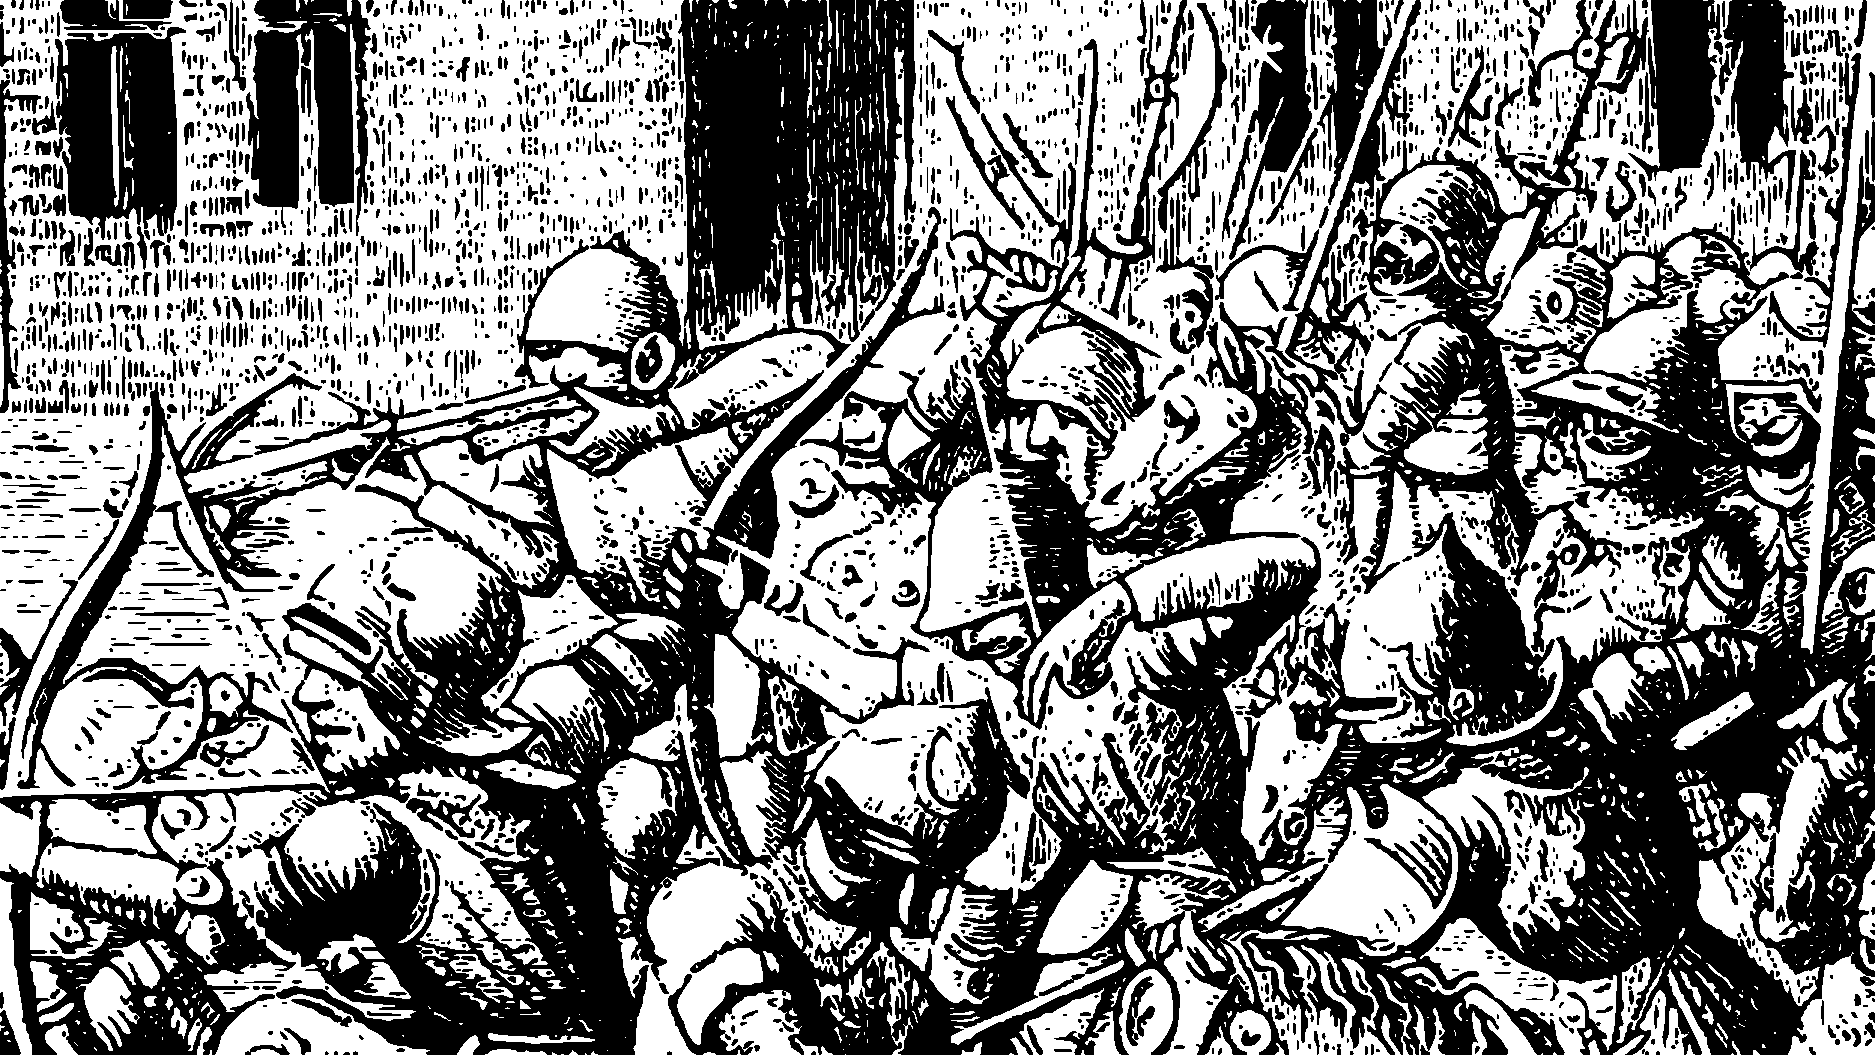
\includegraphics{./images/combat01.pdf}
\caption{Image}
\end{figure}

In Eidos, the combat is based on the ideas presented in this
\href{https://www.youtube.com/watch?v=0o5vWmoS3KU\&ab_channel=SimplyWyvern}{video}.
Basicly the combat needs to be a part of the narrative, not a mini-game
that creates transitions in the game. So there is nothing of initiative
rolls nor anything like that. In the world of Eidos, combat is a dynamic
and immersive experience that forms an integral part of the gameplay.
The combat system in Eidos is meticulously crafted to simulate realistic
combat scenarios, with mechanics that emphasize tactical decision-making
and narrative engagement.

\hypertarget{turn-structure}{%
\subsection{Turn Structure}\label{turn-structure}}

Combat in Eidos follows a fluid turn structure, allowing for seamless
interaction between players and the game master. Unlike traditional
turn-based systems, Eidos prioritizes moment-to-moment decision-making,
where players and the GM exchange actions and reactions in real-time.
This approach enhances the narrative flow of combat scenes, fostering a
sense of urgency and immersion.

\hypertarget{conflic-resolution}{%
\subsection{Conflic Resolution}\label{conflic-resolution}}

Conflict resolution in Eidos is resolved through a combination of dice
rolls and narrative storytelling. Players utilize a 2 20d roll to
determine the outcome of their actions, with results influenced by their
character's skills, abilities, and environmental factors. The DM
adjudicates conflicts based on the narrative context, ensuring that
combat encounters remain dynamic and unpredictable.

\begin{longtable}[]{@{}ll@{}}
\toprule
Difficulty & Target Number \\
\midrule
\endhead
Very easy & 05 \\
Easy & 10 \\
Moderate & 15 \\
Difficult & 20 \\
Hard & 25 \\
Very hard & 30 \\
Extremely hard & 35 \\
Nearly impossible & 39 \\
\bottomrule
\end{longtable}

\begin{figure}
\centering
\includegraphics{./images/combat02.pdf}
\caption{Image}
\end{figure}

\hypertarget{injury-tables}{%
\subsection{Injury Tables}\label{injury-tables}}

Each attack's success prompts a roll on a corresponding injury table.
For example, an attacker aims for a specific body part like the neck and
successfully hits, the player rolls the ``Cutting in Neck Damage Table''
to determine the outcome. These tables define the consequences, ranging
from minor wounds to severe trauma.

\begin{longtable}[]{@{}ll@{}}
\toprule
Type of Damage & Description \\
\midrule
\endhead
Cutting & Damage caused by sharp-edged weapons \\
Stabbing & Damage caused by piercing weapons \\
Impact & Damage from blunt force or crushing attacks \\
Fire & Damage from burns or heat sources \\
Acid & Damage from corrosive acids or chemicals \\
Poison & Damage caused by poison \\
Fall & Damage caused by falling from a tall place \\
\bottomrule
\end{longtable}

\begin{longtable}[]{@{}ll@{}}
\toprule
Body Part & Description \\
\midrule
\endhead
Head & The uppermost part of the body \\
Torso & The main part of the body, including chest \\
Left Arm & The left arm and hand \\
Right Arm & The right arm and hand \\
Left Leg & The left leg and foot \\
Right Leg & The right leg and foot \\
Abdomen & The area between the chest and pelvis \\
Back & The rear part of the torso \\
Neck & The part connecting the head to the body \\
Face & The front of the head, including facial features \\
\bottomrule
\end{longtable}

\begin{figure}
\centering
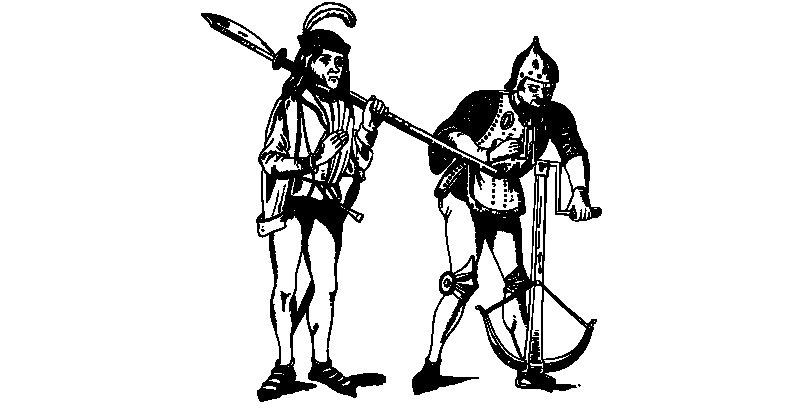
\includegraphics{./images/combat03.pdf}
\caption{Image}
\end{figure}

\hypertarget{cutting}{%
\subsubsection{Cutting}\label{cutting}}

\textbf{Cutting in the Head}

\begin{longtable}[]{@{}
  >{\raggedright\arraybackslash}p{(\columnwidth - 6\tabcolsep) * \real{0.0619}}
  >{\raggedright\arraybackslash}p{(\columnwidth - 6\tabcolsep) * \real{0.5464}}
  >{\raggedright\arraybackslash}p{(\columnwidth - 6\tabcolsep) * \real{0.1753}}
  >{\raggedright\arraybackslash}p{(\columnwidth - 6\tabcolsep) * \real{0.2165}}@{}}
\toprule
\begin{minipage}[b]{\linewidth}\raggedright
Roll
\end{minipage} & \begin{minipage}[b]{\linewidth}\raggedright
Injury Description
\end{minipage} & \begin{minipage}[b]{\linewidth}\raggedright
Recovery Time
\end{minipage} & \begin{minipage}[b]{\linewidth}\raggedright
Scars
\end{minipage} \\
\midrule
\endhead
1 & Minor scalp laceration, blood trickling & 1d4 hours & Light scar \\
2 & Shallow cut on forehead, slight bleeding & 1d4 hours & Small scar \\
3 & Ear nicked, minor pain and bleeding & 1d4 hours & Tiny scar \\
4 & Cheek grazed, minor discomfort & 1d4 hours & Faint scar \\
5 & Eyebrow cut, minor blood and irritation & 1d4 hours & Light scar \\
6 & Nose scratched, slight bleeding & 1d4 hours & Small scar \\
7 & Chin cut, stinging pain and minor blood & 1d4 hours & Tiny scar \\
8 & Forehead gash, bleeding and moderate pain & 1d4 hours & Faint
scar \\
9 & Scalp tear, bleeding and headache & 1d4 hours & Light scar \\
10 & Lip cut, bleeding and mild pain & 1d4 hours & Small scar \\
11 & Deep facial wound, potential scarring & 1d4 days & Visible scar \\
12 & Eye injured, risk of blindness & 1d4 days & Disfiguring scar \\
13 & Skull fracture, severe headache & 1d4 weeks & Permanent damage \\
14 & Head gash, risk of infection & 1d4 weeks & Deep scar \\
15 & Severed artery, immediate death & Instant death & N/A \\
16 & Severe brain injury, instant unconsciousness & Instant death &
N/A \\
17 & Instant brain death, no chance of revival & Instant death & N/A \\
18 & Severe cranial trauma, instant death & Instant death & N/A \\
19 & Critical hit, catastrophic brain damage & Instant death & N/A \\
20 & Critical hit, brain pierced, instant death & Instant death & N/A \\
\bottomrule
\end{longtable}

\begin{figure}
\centering
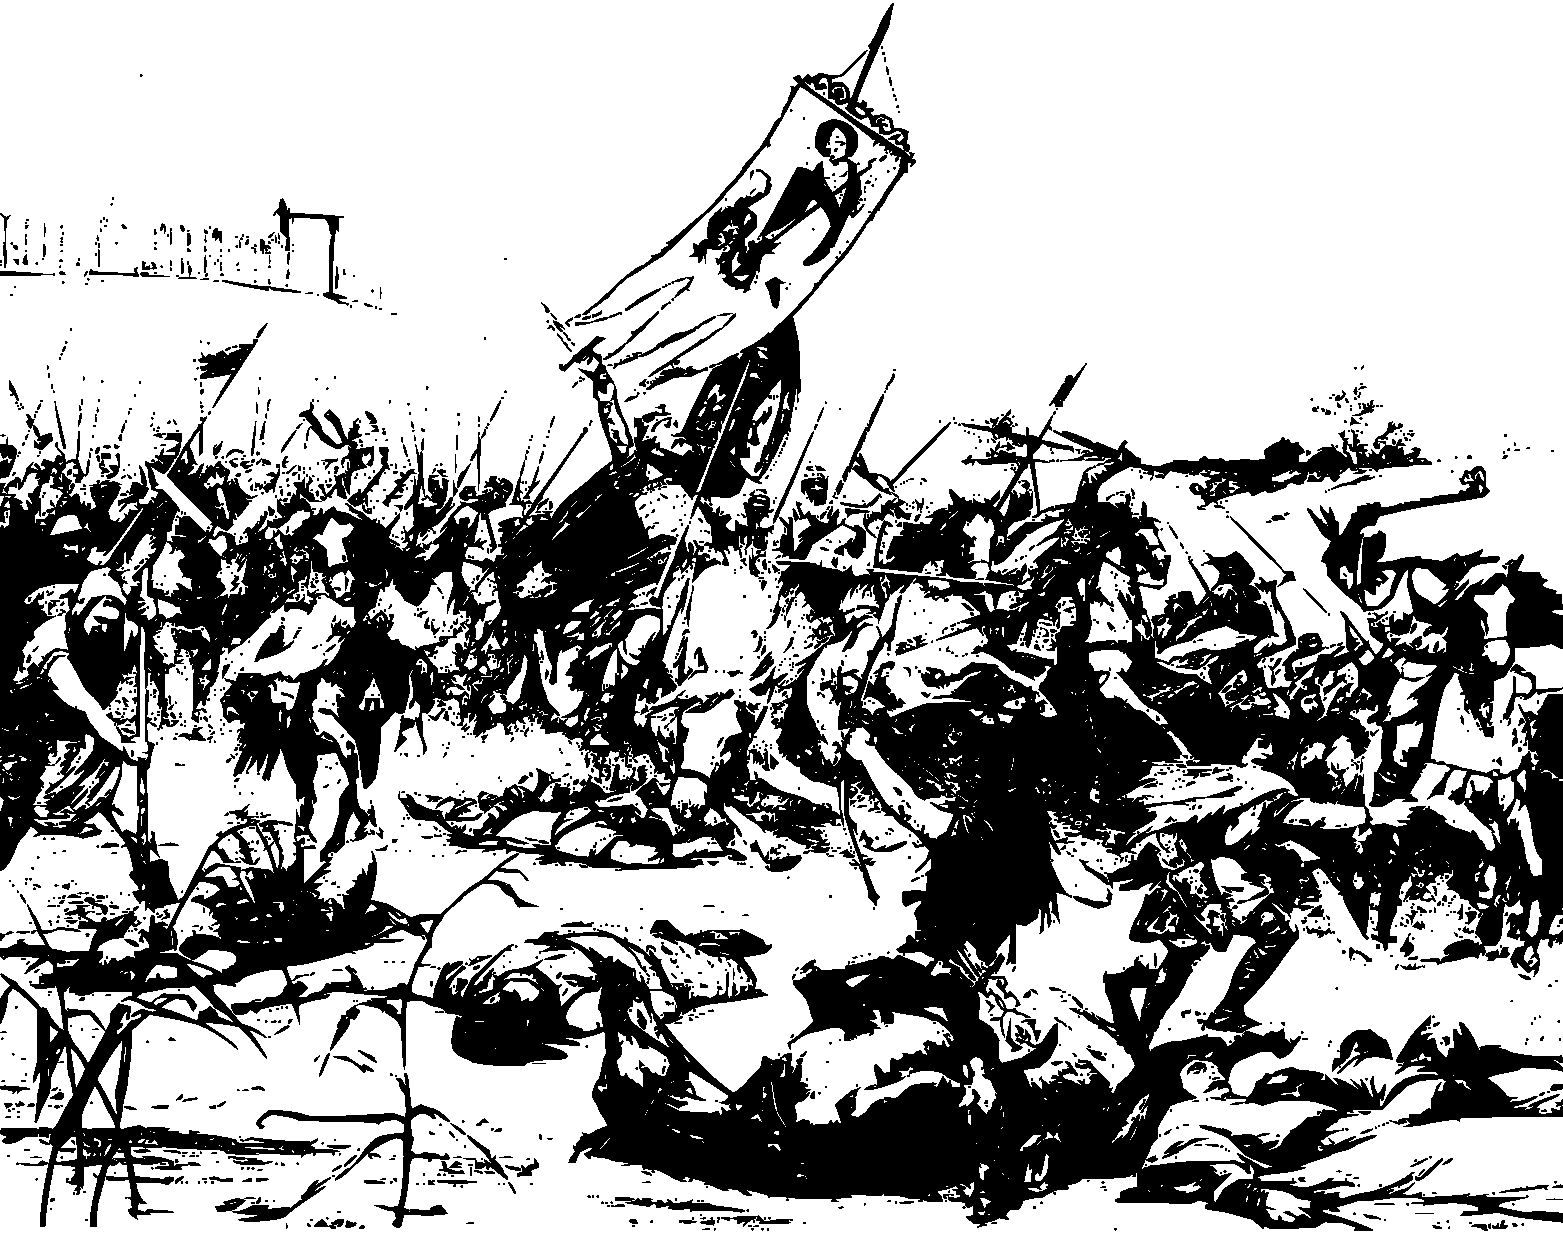
\includegraphics{./images/combat06.pdf}
\caption{Image}
\end{figure}

\textbf{Cutting in the Torso}

\begin{longtable}[]{@{}
  >{\raggedright\arraybackslash}p{(\columnwidth - 6\tabcolsep) * \real{0.0594}}
  >{\raggedright\arraybackslash}p{(\columnwidth - 6\tabcolsep) * \real{0.5644}}
  >{\raggedright\arraybackslash}p{(\columnwidth - 6\tabcolsep) * \real{0.1683}}
  >{\raggedright\arraybackslash}p{(\columnwidth - 6\tabcolsep) * \real{0.2079}}@{}}
\toprule
\begin{minipage}[b]{\linewidth}\raggedright
Roll
\end{minipage} & \begin{minipage}[b]{\linewidth}\raggedright
Injury Description
\end{minipage} & \begin{minipage}[b]{\linewidth}\raggedright
Recovery Time
\end{minipage} & \begin{minipage}[b]{\linewidth}\raggedright
Scars
\end{minipage} \\
\midrule
\endhead
1 & Superficial chest graze, minor pain & 1d4 hours & Faint scar \\
2 & Light abdominal scratch, discomfort & 1d4 hours & Small scar \\
3 & Minor rib cut, mild pain and shallow bleeding & 1d4 hours & Tiny
scar \\
4 & Skin nicked on side, slight irritation & 1d4 hours & Faint scar \\
5 & Chest cut, moderate pain and minor bleeding & 1d4 hours & Light
scar \\
6 & Abdominal laceration, blood trickling & 1d4 hours & Small scar \\
7 & Side wound, moderate pain and bleeding & 1d4 hours & Tiny scar \\
8 & Deep chest gash, significant bleeding & 1d4 days & Faint scar \\
9 & Rib gash, severe pain and bleeding & 1d4 days & Light scar \\
10 & Abdominal cut, potential scarring & 1d4 days & Small scar \\
11 & Organ grazed, risk of infection & 1d4 weeks & Deep scar \\
12 & Punctured lung, difficulty breathing & 1d4 weeks & Permanent
damage \\
13 & Severe internal injury, risk of shock & 1d4 weeks & Visible scar \\
14 & Aorta nicked, rapid blood loss & Instant death & N/A \\
15 & Heart pierced, immediate death & Instant death & N/A \\
16 & Severed spinal cord, instant paralysis & Instant death & N/A \\
17 & Major organ rupture, instant internal bleeding & Instant death &
N/A \\
18 & Critical hit, catastrophic internal damage & Instant death & N/A \\
19 & Critical hit, vital organs obliterated & Instant death & N/A \\
20 & Critical hit, torso sliced open, instant death & Instant death &
N/A \\
\bottomrule
\end{longtable}

\textbf{Cutting in the Arms}

\begin{longtable}[]{@{}
  >{\raggedright\arraybackslash}p{(\columnwidth - 6\tabcolsep) * \real{0.0594}}
  >{\raggedright\arraybackslash}p{(\columnwidth - 6\tabcolsep) * \real{0.5644}}
  >{\raggedright\arraybackslash}p{(\columnwidth - 6\tabcolsep) * \real{0.1683}}
  >{\raggedright\arraybackslash}p{(\columnwidth - 6\tabcolsep) * \real{0.2079}}@{}}
\toprule
\begin{minipage}[b]{\linewidth}\raggedright
Roll
\end{minipage} & \begin{minipage}[b]{\linewidth}\raggedright
Injury Description
\end{minipage} & \begin{minipage}[b]{\linewidth}\raggedright
Recovery Time
\end{minipage} & \begin{minipage}[b]{\linewidth}\raggedright
Scars
\end{minipage} \\
\midrule
\endhead
1 & Superficial arm graze, minor discomfort & 1d4 hours & Faint scar \\
2 & Light forearm scratch, slight pain & 1d4 hours & Small scar \\
3 & Minor hand cut, mild bleeding & 1d4 hours & Tiny scar \\
4 & Skin nicked on upper arm, slight irritation & 1d4 hours & Faint
scar \\
5 & Elbow grazed, moderate pain and minor bleeding & 1d4 hours & Light
scar \\
6 & Wrist scratched, slight bleeding & 1d4 hours & Small scar \\
7 & Finger cut, stinging pain and minor bleeding & 1d4 hours & Tiny
scar \\
8 & Deep forearm gash, significant bleeding & 1d4 days & Faint scar \\
9 & Upper arm cut, severe pain and bleeding & 1d4 days & Light scar \\
10 & Hand laceration, potential scarring & 1d4 days & Small scar \\
11 & Tendon nicked, risk of permanent damage & 1d4 weeks & Deep scar \\
12 & Arterial wound, rapid blood loss & Instant death & N/A \\
13 & Hand mutilation, high risk of infection & Instant death & N/A \\
14 & Severe muscle damage, limited use of arm & 1d4 weeks & Permanent
damage \\
15 & Hand severed, instant death & Instant death & N/A \\
16 & Critical hit, arm sliced off, instant death & Instant death &
N/A \\
17 & Critical hit, arm mutilated, instant death & Instant death & N/A \\
18 & Critical hit, arteries severed, instant death & Instant death &
N/A \\
19 & Critical hit, shattered bones, instant death & Instant death &
N/A \\
20 & Critical hit, arm disintegrated, instant death & Instant death &
N/A \\
\bottomrule
\end{longtable}

\begin{figure}
\centering
\includegraphics{./images/combat07.pdf}
\caption{Image}
\end{figure}

\textbf{Cutting in the Legs}

\begin{longtable}[]{@{}
  >{\raggedright\arraybackslash}p{(\columnwidth - 6\tabcolsep) * \real{0.0588}}
  >{\raggedright\arraybackslash}p{(\columnwidth - 6\tabcolsep) * \real{0.5686}}
  >{\raggedright\arraybackslash}p{(\columnwidth - 6\tabcolsep) * \real{0.1667}}
  >{\raggedright\arraybackslash}p{(\columnwidth - 6\tabcolsep) * \real{0.2059}}@{}}
\toprule
\begin{minipage}[b]{\linewidth}\raggedright
Roll
\end{minipage} & \begin{minipage}[b]{\linewidth}\raggedright
Injury Description
\end{minipage} & \begin{minipage}[b]{\linewidth}\raggedright
Recovery Time
\end{minipage} & \begin{minipage}[b]{\linewidth}\raggedright
Scars
\end{minipage} \\
\midrule
\endhead
1 & Superficial thigh graze, minor discomfort & 1d4 hours & Faint
scar \\
2 & Light calf scratch, slight pain & 1d4 hours & Small scar \\
3 & Minor ankle cut, mild bleeding & 1d4 hours & Tiny scar \\
4 & Skin nicked on shin, slight irritation & 1d4 hours & Faint scar \\
5 & Knee grazed, moderate pain and minor bleeding & 1d4 hours & Light
scar \\
6 & Heel scratched, slight bleeding & 1d4 hours & Small scar \\
7 & Toe cut, stinging pain and minor bleeding & 1d4 hours & Tiny scar \\
8 & Deep thigh gash, significant bleeding & 1d4 days & Faint scar \\
9 & Calf cut, severe pain and bleeding & 1d4 days & Light scar \\
10 & Ankle laceration, potential scarring & 1d4 days & Small scar \\
11 & Tendon severed, risk of permanent damage & 1d4 weeks & Deep scar \\
12 & Arterial wound, rapid blood loss & Instant death & N/A \\
13 & Leg mutilation, high risk of infection & Instant death & N/A \\
14 & Severe muscle damage, limited mobility & 1d4 weeks & Permanent
damage \\
15 & Leg severed, instant death & Instant death & N/A \\
16 & Critical hit, leg sliced off, instant death & Instant death &
N/A \\
17 & Critical hit, leg mutilated, instant death & Instant death & N/A \\
18 & Critical hit, arteries severed, instant death & Instant death &
N/A \\
19 & Critical hit, shattered bones, instant death & Instant death &
N/A \\
20 & Critical hit, leg disintegrated, instant death & Instant death &
N/A \\
\bottomrule
\end{longtable}

\begin{figure}
\centering
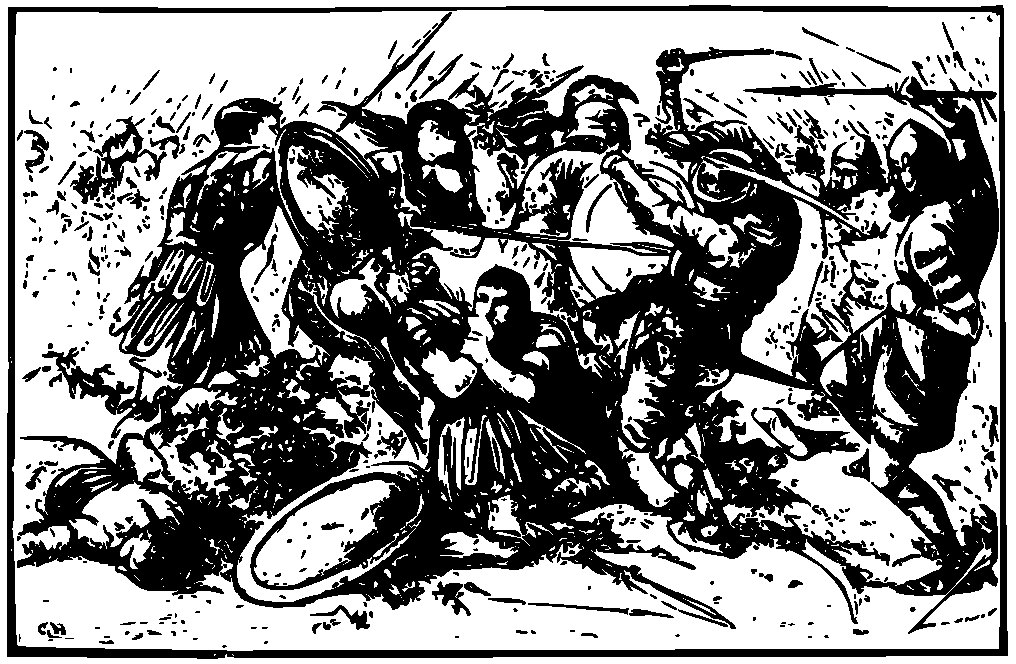
\includegraphics{./images/combat04.pdf}
\caption{Image}
\end{figure}

\textbf{Cutting in the Abdomen}

\begin{longtable}[]{@{}
  >{\raggedright\arraybackslash}p{(\columnwidth - 6\tabcolsep) * \real{0.0606}}
  >{\raggedright\arraybackslash}p{(\columnwidth - 6\tabcolsep) * \real{0.5556}}
  >{\raggedright\arraybackslash}p{(\columnwidth - 6\tabcolsep) * \real{0.1717}}
  >{\raggedright\arraybackslash}p{(\columnwidth - 6\tabcolsep) * \real{0.2121}}@{}}
\toprule
\begin{minipage}[b]{\linewidth}\raggedright
Roll
\end{minipage} & \begin{minipage}[b]{\linewidth}\raggedright
Injury Description
\end{minipage} & \begin{minipage}[b]{\linewidth}\raggedright
Recovery Time
\end{minipage} & \begin{minipage}[b]{\linewidth}\raggedright
Scars
\end{minipage} \\
\midrule
\endhead
1 & Superficial scratch, minor discomfort & 1d4 hours & Light scar \\
2 & Shallow cut, light bleeding and mild pain & 1d4 hours & Small
scar \\
3 & Glancing blow, minimal bleeding & 1d4 hours & Tiny scar \\
4 & Skin nicked, slight pain and minor bleeding & 1d4 hours & Faint
scar \\
5 & Grazed wound, bleeding and moderate pain & 1d4 hours & Light scar \\
6 & Sliced flesh, steady bleeding and discomfort & 1d4 hours & Small
scar \\
7 & Deep cut, significant pain and bleeding & 1d4 hours & Tiny scar \\
8 & Muscle incision, bleeding and throbbing pain & 1d4 hours & Faint
scar \\
9 & Torn flesh, profuse bleeding and severe pain & 1d4 days & Light
scar \\
10 & Severe laceration, risk of infection and agony & 1d4 days & Small
scar \\
11 & Ruptured muscle, intense pain and internal bleeding & 1d4 days &
Visible scar \\
12 & Organ grazed, danger of internal complications & 1d4 weeks & Deep
scar \\
13 & Severed artery, rapid blood loss and shock & 1d4 weeks & Permanent
damage \\
14 & Major organ damage, critical condition & 1d4 weeks & Life-altering
scar \\
15 & Perforated intestine, septicemia and extreme pain & Instant death &
N/A \\
16 & Ruptured kidney, internal hemorrhage and shock & Instant death &
N/A \\
17 & Impaled aorta, rapid exsanguination and agony & Instant death &
N/A \\
18 & Critical hit, disembowelment and instant death & Instant death &
N/A \\
19 & Critical hit, evisceration and instant death & Instant death &
N/A \\
20 & Critical hit, shredded organs and instant death & Instant death &
N/A \\
\bottomrule
\end{longtable}

\textbf{Cutting in the Back}

\begin{longtable}[]{@{}
  >{\raggedright\arraybackslash}p{(\columnwidth - 6\tabcolsep) * \real{0.0594}}
  >{\raggedright\arraybackslash}p{(\columnwidth - 6\tabcolsep) * \real{0.5644}}
  >{\raggedright\arraybackslash}p{(\columnwidth - 6\tabcolsep) * \real{0.1683}}
  >{\raggedright\arraybackslash}p{(\columnwidth - 6\tabcolsep) * \real{0.2079}}@{}}
\toprule
\begin{minipage}[b]{\linewidth}\raggedright
Roll
\end{minipage} & \begin{minipage}[b]{\linewidth}\raggedright
Injury Description
\end{minipage} & \begin{minipage}[b]{\linewidth}\raggedright
Recovery Time
\end{minipage} & \begin{minipage}[b]{\linewidth}\raggedright
Scars
\end{minipage} \\
\midrule
\endhead
1 & Superficial scratch, minor discomfort & 1d4 hours & Light scar \\
2 & Shallow cut, light bleeding and mild pain & 1d4 hours & Small
scar \\
3 & Skin grazed, slight pain and minor bleeding & 1d4 hours & Tiny
scar \\
4 & Flesh nicked, minor discomfort & 1d4 hours & Faint scar \\
5 & Surface cut, bleeding and moderate pain & 1d4 hours & Light scar \\
6 & Muscle graze, slight bleeding and irritation & 1d4 hours & Small
scar \\
7 & Deep cut, significant pain and bleeding & 1d4 hours & Tiny scar \\
8 & Tendon nicked, bleeding and throbbing pain & 1d4 hours & Faint
scar \\
9 & Muscle laceration, bleeding and discomfort & 1d4 days & Light
scar \\
10 & Nerve cut, risk of partial paralysis and agony & 1d4 days & Small
scar \\
11 & Ruptured muscle, intense pain and internal bleeding & 1d4 days &
Visible scar \\
12 & Organ grazed, potential internal complications & 1d4 weeks & Deep
scar \\
13 & Major artery cut, rapid blood loss and shock & 1d4 weeks &
Permanent damage \\
14 & Spinal injury, paralysis risk and extreme pain & 1d4 weeks &
Life-altering scar \\
15 & Severed spine, instant paralysis and agony & Instant death & N/A \\
16 & Critical hit, spine shattered, instant death & Instant death &
N/A \\
17 & Critical hit, spine pierced, instant death & Instant death & N/A \\
18 & Critical hit, vital organ pierced, instant death & Instant death &
N/A \\
19 & Critical hit, disembowelment and instant death & Instant death &
N/A \\
20 & Critical hit, catastrophic spinal trauma and death & Instant death
& N/A \\
\bottomrule
\end{longtable}

\begin{figure}
\centering
\includegraphics{./images/combat08.pdf}
\caption{Image}
\end{figure}

\textbf{Cutting in the Neck}

\begin{longtable}[]{@{}
  >{\raggedright\arraybackslash}p{(\columnwidth - 6\tabcolsep) * \real{0.0632}}
  >{\raggedright\arraybackslash}p{(\columnwidth - 6\tabcolsep) * \real{0.5368}}
  >{\raggedright\arraybackslash}p{(\columnwidth - 6\tabcolsep) * \real{0.1789}}
  >{\raggedright\arraybackslash}p{(\columnwidth - 6\tabcolsep) * \real{0.2211}}@{}}
\toprule
\begin{minipage}[b]{\linewidth}\raggedright
Roll
\end{minipage} & \begin{minipage}[b]{\linewidth}\raggedright
Injury Description
\end{minipage} & \begin{minipage}[b]{\linewidth}\raggedright
Recovery Time
\end{minipage} & \begin{minipage}[b]{\linewidth}\raggedright
Scars
\end{minipage} \\
\midrule
\endhead
1 & Skin nick, minor discomfort & 1d4 hours & Light scar \\
2 & Shallow cut, light bleeding and mild pain & 1d4 hours & Small
scar \\
3 & Neck graze, slight pain and minor bleeding & 1d4 hours & Tiny
scar \\
4 & Flesh cut, minor discomfort & 1d4 hours & Faint scar \\
5 & Surface wound, bleeding and moderate pain & 1d4 hours & Light
scar \\
6 & Muscle nick, slight bleeding and irritation & 1d4 hours & Small
scar \\
7 & Deep gash, significant pain and bleeding & 1d4 hours & Tiny scar \\
8 & Carotid artery cut, rapid blood loss & Instant death & N/A \\
9 & Jugular vein cut, severe blood loss & Instant death & N/A \\
10 & Windpipe nick, difficulty breathing & 1d4 days & Light scar \\
11 & Nerve damage, risk of partial paralysis & 1d4 days & Small scar \\
12 & Critical hit, trachea crushed, instant death & Instant death &
N/A \\
13 & Critical hit, spinal cord severed, death & Instant death & N/A \\
14 & Critical hit, catastrophic blood loss & Instant death & N/A \\
15 & Critical hit, catastrophic muscle damage & Instant death & N/A \\
16 & Critical hit, major artery cut, instant death & Instant death &
N/A \\
17 & Critical hit, dissection of vital organs & Instant death & N/A \\
18 & Critical hit, decapitation, instant death & Instant death & N/A \\
19 & Critical hit, mutilation, instant death & Instant death & N/A \\
20 & Critical hit, neck shattered, instant death & Instant death &
N/A \\
\bottomrule
\end{longtable}

\textbf{Cutting in the Face}

\begin{longtable}[]{@{}
  >{\raggedright\arraybackslash}p{(\columnwidth - 6\tabcolsep) * \real{0.0625}}
  >{\raggedright\arraybackslash}p{(\columnwidth - 6\tabcolsep) * \real{0.5417}}
  >{\raggedright\arraybackslash}p{(\columnwidth - 6\tabcolsep) * \real{0.1771}}
  >{\raggedright\arraybackslash}p{(\columnwidth - 6\tabcolsep) * \real{0.2188}}@{}}
\toprule
\begin{minipage}[b]{\linewidth}\raggedright
Roll
\end{minipage} & \begin{minipage}[b]{\linewidth}\raggedright
Injury Description
\end{minipage} & \begin{minipage}[b]{\linewidth}\raggedright
Recovery Time
\end{minipage} & \begin{minipage}[b]{\linewidth}\raggedright
Scars
\end{minipage} \\
\midrule
\endhead
1 & Superficial scratch, minor discomfort & 1d4 hours & Light scar \\
2 & Shallow cut, light bleeding and mild pain & 1d4 hours & Small
scar \\
3 & Skin grazed, slight pain and minor bleeding & 1d4 hours & Tiny
scar \\
4 & Cheek cut, minor discomfort & 1d4 hours & Faint scar \\
5 & Eyebrow nick, minor blood and irritation & 1d4 hours & Light scar \\
6 & Nose scratch, slight bleeding & 1d4 hours & Small scar \\
7 & Lip gash, stinging pain and minor bleeding & 1d4 hours & Tiny
scar \\
8 & Forehead wound, bleeding and moderate pain & 1d4 hours & Faint
scar \\
9 & Eye injury, risk of blindness & 1d4 days & Disfiguring scar \\
10 & Deep facial wound, potential scarring & 1d4 days & Visible scar \\
11 & Facial nerve damage, risk of paralysis & 1d4 days & Permanent
damage \\
12 & Critical hit, eye socket shattered, death & Instant death & N/A \\
13 & Critical hit, facial bones crushed, death & Instant death & N/A \\
14 & Critical hit, disfigurement, death & Instant death & N/A \\
15 & Critical hit, brain exposed, instant death & Instant death & N/A \\
16 & Critical hit, catastrophic facial trauma & Instant death & N/A \\
17 & Critical hit, mutilation, instant death & Instant death & N/A \\
18 & Critical hit, jaw disintegration, instant death & Instant death &
N/A \\
19 & Critical hit, facial dismemberment, instant death & Instant death &
N/A \\
20 & Critical hit, head severed, instant death & Instant death & N/A \\
\bottomrule
\end{longtable}

\begin{figure}
\centering
\includegraphics{./images/combat09.pdf}
\caption{Image}
\end{figure}

\hypertarget{stabbing}{%
\subsubsection{Stabbing}\label{stabbing}}

\textbf{Stabbing in the Head}

\begin{longtable}[]{@{}
  >{\raggedright\arraybackslash}p{(\columnwidth - 6\tabcolsep) * \real{0.0619}}
  >{\raggedright\arraybackslash}p{(\columnwidth - 6\tabcolsep) * \real{0.5464}}
  >{\raggedright\arraybackslash}p{(\columnwidth - 6\tabcolsep) * \real{0.1753}}
  >{\raggedright\arraybackslash}p{(\columnwidth - 6\tabcolsep) * \real{0.2165}}@{}}
\toprule
\begin{minipage}[b]{\linewidth}\raggedright
Roll
\end{minipage} & \begin{minipage}[b]{\linewidth}\raggedright
Injury Description
\end{minipage} & \begin{minipage}[b]{\linewidth}\raggedright
Recovery Time
\end{minipage} & \begin{minipage}[b]{\linewidth}\raggedright
Scars
\end{minipage} \\
\midrule
\endhead
1 & Grazed scalp, minor pain & 1d4 hours & Light scar \\
2 & Superficial forehead stab, slight bleeding & 1d4 hours & Small
scar \\
3 & Ear nicked, minor pain and bleeding & 1d4 hours & Tiny scar \\
4 & Cheek stab, minor discomfort & 1d4 hours & Faint scar \\
5 & Eyebrow pierced, minor blood and irritation & 1d4 hours & Light
scar \\
6 & Nose scratched, slight bleeding & 1d4 hours & Small scar \\
7 & Jaw hit, stinging pain and minor blood & 1d4 hours & Tiny scar \\
8 & Forehead stab, bleeding and moderate pain & 1d4 hours & Faint
scar \\
9 & Scalp puncture, bleeding and headache & 1d4 hours & Light scar \\
10 & Lip puncture, bleeding and mild pain & 1d4 hours & Small scar \\
11 & Eye injured, risk of blindness & 1d4 days & Disfiguring scar \\
12 & Critical hit, eye socket impaled, instant death & Instant death &
N/A \\
13 & Critical hit, brain impaled, instant death & Instant death & N/A \\
14 & Critical hit, cranial fracture, instant death & Instant death &
N/A \\
15 & Critical hit, brain penetration, instant death & Instant death &
N/A \\
16 & Critical hit, catastrophic brain damage & Instant death & N/A \\
17 & Critical hit, skull shattered, instant death & Instant death &
N/A \\
18 & Critical hit, brain dissection, instant death & Instant death &
N/A \\
19 & Critical hit, cerebral rupture, instant death & Instant death &
N/A \\
20 & Critical hit, decapitation, instant death & Instant death & N/A \\
\bottomrule
\end{longtable}

\textbf{Stabbing in the Torso}

\begin{longtable}[]{@{}
  >{\raggedright\arraybackslash}p{(\columnwidth - 6\tabcolsep) * \real{0.0600}}
  >{\raggedright\arraybackslash}p{(\columnwidth - 6\tabcolsep) * \real{0.5400}}
  >{\raggedright\arraybackslash}p{(\columnwidth - 6\tabcolsep) * \real{0.1800}}
  >{\raggedright\arraybackslash}p{(\columnwidth - 6\tabcolsep) * \real{0.2200}}@{}}
\toprule
\begin{minipage}[b]{\linewidth}\raggedright
Roll
\end{minipage} & \begin{minipage}[b]{\linewidth}\raggedright
Injury Description
\end{minipage} & \begin{minipage}[b]{\linewidth}\raggedright
Recovery Time
\end{minipage} & \begin{minipage}[b]{\linewidth}\raggedright
Scars
\end{minipage} \\
\midrule
\endhead
1 & Superficial abdominal graze, minor discomfort & 1d4 hours & Light
scar \\
2 & Shallow chest cut, slight bleeding & 1d4 hours & Small scar \\
3 & Rib nicked, minor pain and bleeding & 1d4 hours & Tiny scar \\
4 & Belly graze, minor pain and irritation & 1d4 hours & Faint scar \\
5 & Abdominal cut, minor bleeding and discomfort & 1d4 hours & Light
scar \\
6 & Diaphragm scratch, slight bleeding & 1d4 hours & Small scar \\
7 & Lower abdomen stab, stinging pain and blood & 1d4 hours & Tiny
scar \\
8 & Chest puncture, moderate pain and bleeding & 1d4 hours & Faint
scar \\
9 & Gut wound, bleeding and abdominal pain & 1d4 hours & Light scar \\
10 & Side stab, bleeding and moderate pain & 1d4 hours & Small scar \\
11 & Lung punctured, breathing difficulties & 1d4 days & Visible scar \\
12 & Liver injury, internal bleeding risk & 1d4 days & Disfiguring
scar \\
13 & Critical hit, heart pierced, instant death & Instant death & N/A \\
14 & Critical hit, major organ damage, instant death & Instant death &
N/A \\
15 & Critical hit, arterial rupture, instant death & Instant death &
N/A \\
16 & Critical hit, spine punctured, instant death & Instant death &
N/A \\
17 & Critical hit, disembowelment, instant death & Instant death &
N/A \\
18 & Critical hit, massive hemorrhage, instant death & Instant death &
N/A \\
19 & Critical hit, vital artery sliced, instant death & Instant death &
N/A \\
20 & Critical hit, impaled through heart, instant death & Instant death
& N/A \\
\bottomrule
\end{longtable}

\begin{figure}
\centering
\includegraphics{./images/combat10.pdf}
\caption{Image}
\end{figure}

\textbf{Stabbing in the Arms}

\begin{longtable}[]{@{}
  >{\raggedright\arraybackslash}p{(\columnwidth - 6\tabcolsep) * \real{0.0625}}
  >{\raggedright\arraybackslash}p{(\columnwidth - 6\tabcolsep) * \real{0.5417}}
  >{\raggedright\arraybackslash}p{(\columnwidth - 6\tabcolsep) * \real{0.1771}}
  >{\raggedright\arraybackslash}p{(\columnwidth - 6\tabcolsep) * \real{0.2188}}@{}}
\toprule
\begin{minipage}[b]{\linewidth}\raggedright
Roll
\end{minipage} & \begin{minipage}[b]{\linewidth}\raggedright
Injury Description
\end{minipage} & \begin{minipage}[b]{\linewidth}\raggedright
Recovery Time
\end{minipage} & \begin{minipage}[b]{\linewidth}\raggedright
Scars
\end{minipage} \\
\midrule
\endhead
1 & Superficial arm graze, minor discomfort & 1d4 hours & Light scar \\
2 & Shallow cut on forearm, slight bleeding & 1d4 hours & Small scar \\
3 & Arm nicked, minor pain and bleeding & 1d4 hours & Tiny scar \\
4 & Elbow grazed, minor pain and irritation & 1d4 hours & Faint scar \\
5 & Wrist cut, minor bleeding and discomfort & 1d4 hours & Light scar \\
6 & Knuckle scratched, slight bleeding & 1d4 hours & Small scar \\
7 & Palm cut, stinging pain and minor blood & 1d4 hours & Tiny scar \\
8 & Forearm gash, moderate pain and bleeding & 1d4 hours & Faint scar \\
9 & Bicep tear, bleeding and muscle ache & 1d4 hours & Light scar \\
10 & Shoulder cut, bleeding and discomfort & 1d4 hours & Small scar \\
11 & Major artery nicked, immediate medical aid & 1d4 days & Visible
scar \\
12 & Severe nerve damage, loss of sensation & 1d4 days & Disfiguring
scar \\
13 & Critical hit, artery severed, instant death & Instant death &
N/A \\
14 & Critical hit, nerve cluster damaged & Instant death & N/A \\
15 & Critical hit, major blood loss, instant death & Instant death &
N/A \\
16 & Critical hit, limb paralyzed, instant death & Instant death &
N/A \\
17 & Critical hit, shattered bone, instant death & Instant death &
N/A \\
18 & Critical hit, limb dismembered, instant death & Instant death &
N/A \\
19 & Critical hit, vital artery pierced, instant death & Instant death &
N/A \\
20 & Critical hit, arm impaled, instant death & Instant death & N/A \\
\bottomrule
\end{longtable}

\textbf{Stabbing in the Legs}

\begin{longtable}[]{@{}
  >{\raggedright\arraybackslash}p{(\columnwidth - 6\tabcolsep) * \real{0.0625}}
  >{\raggedright\arraybackslash}p{(\columnwidth - 6\tabcolsep) * \real{0.5417}}
  >{\raggedright\arraybackslash}p{(\columnwidth - 6\tabcolsep) * \real{0.1771}}
  >{\raggedright\arraybackslash}p{(\columnwidth - 6\tabcolsep) * \real{0.2188}}@{}}
\toprule
\begin{minipage}[b]{\linewidth}\raggedright
Roll
\end{minipage} & \begin{minipage}[b]{\linewidth}\raggedright
Injury Description
\end{minipage} & \begin{minipage}[b]{\linewidth}\raggedright
Recovery Time
\end{minipage} & \begin{minipage}[b]{\linewidth}\raggedright
Scars
\end{minipage} \\
\midrule
\endhead
1 & Leg scratch, minor discomfort & 1d4 hours & Light scar \\
2 & Calf graze, slight bleeding & 1d4 hours & Small scar \\
3 & Ankle nicked, minor pain and bleeding & 1d4 hours & Tiny scar \\
4 & Knee scraped, minor pain and irritation & 1d4 hours & Faint scar \\
5 & Shin cut, minor bleeding and discomfort & 1d4 hours & Light scar \\
6 & Thigh scratched, slight bleeding & 1d4 hours & Small scar \\
7 & Foot cut, stinging pain and minor blood & 1d4 hours & Tiny scar \\
8 & Upper leg gash, moderate pain and bleeding & 1d4 hours & Faint
scar \\
9 & Hamstring tear, bleeding and muscle ache & 1d4 hours & Light scar \\
10 & Groin cut, bleeding and discomfort & 1d4 hours & Small scar \\
11 & Major vein nicked, immediate medical aid & 1d4 days & Visible
scar \\
12 & Severe nerve damage, impaired mobility & 1d4 days & Disfiguring
scar \\
13 & Critical hit, artery severed, instant death & Instant death &
N/A \\
14 & Critical hit, major nerve damaged & Instant death & N/A \\
15 & Critical hit, massive blood loss, instant death & Instant death &
N/A \\
16 & Critical hit, leg paralyzed, instant death & Instant death & N/A \\
17 & Critical hit, shattered bone, instant death & Instant death &
N/A \\
18 & Critical hit, leg dismembered, instant death & Instant death &
N/A \\
19 & Critical hit, vital artery pierced, instant death & Instant death &
N/A \\
20 & Critical hit, leg impaled, instant death & Instant death & N/A \\
\bottomrule
\end{longtable}

\textbf{Stabbing in The Abdomen}

\begin{longtable}[]{@{}
  >{\raggedright\arraybackslash}p{(\columnwidth - 6\tabcolsep) * \real{0.0606}}
  >{\raggedright\arraybackslash}p{(\columnwidth - 6\tabcolsep) * \real{0.5556}}
  >{\raggedright\arraybackslash}p{(\columnwidth - 6\tabcolsep) * \real{0.1717}}
  >{\raggedright\arraybackslash}p{(\columnwidth - 6\tabcolsep) * \real{0.2121}}@{}}
\toprule
\begin{minipage}[b]{\linewidth}\raggedright
Roll
\end{minipage} & \begin{minipage}[b]{\linewidth}\raggedright
Injury Description
\end{minipage} & \begin{minipage}[b]{\linewidth}\raggedright
Recovery Time
\end{minipage} & \begin{minipage}[b]{\linewidth}\raggedright
Scars
\end{minipage} \\
\midrule
\endhead
1 & Minor abdominal scratch, slight discomfort & 1d4 hours & Light
scar \\
2 & Belly skin nicked, mild bleeding & 1d4 hours & Small scar \\
3 & Navel area cut, minor pain and bleeding & 1d4 hours & Tiny scar \\
4 & Side grazed, minor pain and discomfort & 1d4 hours & Faint scar \\
5 & Lower abdomen cut, minor bleeding and irritation & 1d4 hours & Light
scar \\
6 & Hip scratched, slight bleeding & 1d4 hours & Small scar \\
7 & Waistline cut, stinging pain and minor blood & 1d4 hours & Tiny
scar \\
8 & Upper abdomen wound, moderate pain and bleeding & 1d4 hours & Faint
scar \\
9 & Deep abdominal laceration, internal discomfort & 1d4 hours & Light
scar \\
10 & Flank cut, bleeding and mild pain & 1d4 hours & Small scar \\
11 & Internal bleeding, urgent medical aid needed & 1d4 days & Visible
scar \\
12 & Peritonitis risk, prolonged medical attention & 1d4 days &
Disfiguring scar \\
13 & Critical hit, major organ punctured & Instant death & N/A \\
14 & Critical hit, vital artery slashed & Instant death & N/A \\
15 & Critical hit, massive internal bleeding & Instant death & N/A \\
16 & Critical hit, organ rupture, instant death & Instant death & N/A \\
17 & Critical hit, disembowelment, instant death & Instant death &
N/A \\
18 & Critical hit, abdominal explosion, instant death & Instant death &
N/A \\
19 & Critical hit, instant organ failure, instant death & Instant death
& N/A \\
20 & Critical hit, internal organs impaled, instant death & Instant
death & N/A \\
\bottomrule
\end{longtable}

\textbf{Stabbing in the Back}

\begin{longtable}[]{@{}
  >{\raggedright\arraybackslash}p{(\columnwidth - 6\tabcolsep) * \real{0.0606}}
  >{\raggedright\arraybackslash}p{(\columnwidth - 6\tabcolsep) * \real{0.5556}}
  >{\raggedright\arraybackslash}p{(\columnwidth - 6\tabcolsep) * \real{0.1717}}
  >{\raggedright\arraybackslash}p{(\columnwidth - 6\tabcolsep) * \real{0.2121}}@{}}
\toprule
\begin{minipage}[b]{\linewidth}\raggedright
Roll
\end{minipage} & \begin{minipage}[b]{\linewidth}\raggedright
Injury Description
\end{minipage} & \begin{minipage}[b]{\linewidth}\raggedright
Recovery Time
\end{minipage} & \begin{minipage}[b]{\linewidth}\raggedright
Scars
\end{minipage} \\
\midrule
\endhead
1 & Superficial back scratch, minor discomfort & 1d4 hours & Light
scar \\
2 & Back skin nicked, slight bleeding & 1d4 hours & Small scar \\
3 & Shoulder grazed, minor pain and irritation & 1d4 hours & Tiny
scar \\
4 & Lower back scratch, minor pain and discomfort & 1d4 hours & Faint
scar \\
5 & Spinal area cut, minor bleeding and irritation & 1d4 hours & Light
scar \\
6 & Upper back scratch, slight bleeding & 1d4 hours & Small scar \\
7 & Mid-back cut, stinging pain and minor blood & 1d4 hours & Tiny
scar \\
8 & Deep back wound, moderate pain and bleeding & 1d4 hours & Faint
scar \\
9 & Punctured lung, labored breathing & 1d4 hours & Light scar \\
10 & Kidney area cut, bleeding and mild pain & 1d4 hours & Small scar \\
11 & Severed spine, instant paralysis & Instant death & N/A \\
12 & Critical hit, major organ damage & Instant death & N/A \\
13 & Critical hit, spinal cord severed & Instant death & N/A \\
14 & Critical hit, internal bleeding & Instant death & N/A \\
15 & Critical hit, vital artery punctured & Instant death & N/A \\
16 & Critical hit, instant organ failure & Instant death & N/A \\
17 & Critical hit, immediate paralysis & Instant death & N/A \\
18 & Critical hit, internal damage, instant death & Instant death &
N/A \\
19 & Critical hit, catastrophic spine injury & Instant death & N/A \\
20 & Critical hit, spine shattered, instant death & Instant death &
N/A \\
\bottomrule
\end{longtable}

\textbf{Stabbing in the Neck}

\begin{longtable}[]{@{}
  >{\raggedright\arraybackslash}p{(\columnwidth - 6\tabcolsep) * \real{0.0612}}
  >{\raggedright\arraybackslash}p{(\columnwidth - 6\tabcolsep) * \real{0.5510}}
  >{\raggedright\arraybackslash}p{(\columnwidth - 6\tabcolsep) * \real{0.1735}}
  >{\raggedright\arraybackslash}p{(\columnwidth - 6\tabcolsep) * \real{0.2143}}@{}}
\toprule
\begin{minipage}[b]{\linewidth}\raggedright
Roll
\end{minipage} & \begin{minipage}[b]{\linewidth}\raggedright
Injury Description
\end{minipage} & \begin{minipage}[b]{\linewidth}\raggedright
Recovery Time
\end{minipage} & \begin{minipage}[b]{\linewidth}\raggedright
Scars
\end{minipage} \\
\midrule
\endhead
1 & Neck graze, minor pain and discomfort & 1d4 hours & Light scar \\
2 & Shallow neck cut, slight bleeding & 1d4 hours & Small scar \\
3 & Neck scratch, minor irritation & 1d4 hours & Tiny scar \\
4 & Superficial neck wound, slight pain & 1d4 hours & Faint scar \\
5 & Neck nicked, minor blood and discomfort & 1d4 hours & Light scar \\
6 & Throat scratched, slight bleeding & 1d4 hours & Small scar \\
7 & Neck cut, stinging pain and moderate bleeding & 1d4 hours & Tiny
scar \\
8 & Severe neck wound, bleeding and pain & 1d4 hours & Faint scar \\
9 & Severed artery, immediate death & Instant death & N/A \\
10 & Critical hit, major blood vessel hit & Instant death & N/A \\
11 & Critical hit, spinal cord severed & Instant death & N/A \\
12 & Critical hit, windpipe crushed & Instant death & N/A \\
13 & Critical hit, jugular vein severed & Instant death & N/A \\
14 & Critical hit, instant paralysis & Instant death & N/A \\
15 & Critical hit, catastrophic bleeding & Instant death & N/A \\
16 & Critical hit, severe pain and instant death & Instant death &
N/A \\
17 & Critical hit, airway blocked & Instant death & N/A \\
18 & Critical hit, massive internal damage & Instant death & N/A \\
19 & Critical hit, neck shattered & Instant death & N/A \\
20 & Critical hit, decapitation & Instant death & N/A \\
\bottomrule
\end{longtable}

\textbf{Stabbing in The Face}

\begin{longtable}[]{@{}
  >{\raggedright\arraybackslash}p{(\columnwidth - 6\tabcolsep) * \real{0.0619}}
  >{\raggedright\arraybackslash}p{(\columnwidth - 6\tabcolsep) * \real{0.5464}}
  >{\raggedright\arraybackslash}p{(\columnwidth - 6\tabcolsep) * \real{0.1753}}
  >{\raggedright\arraybackslash}p{(\columnwidth - 6\tabcolsep) * \real{0.2165}}@{}}
\toprule
\begin{minipage}[b]{\linewidth}\raggedright
Roll
\end{minipage} & \begin{minipage}[b]{\linewidth}\raggedright
Injury Description
\end{minipage} & \begin{minipage}[b]{\linewidth}\raggedright
Recovery Time
\end{minipage} & \begin{minipage}[b]{\linewidth}\raggedright
Scars
\end{minipage} \\
\midrule
\endhead
1 & Facial graze, minor pain and discomfort & 1d4 hours & Light scar \\
2 & Superficial cheek cut, slight bleeding & 1d4 hours & Small scar \\
3 & Lip nicked, minor pain and bleeding & 1d4 hours & Tiny scar \\
4 & Nostril scratched, minor irritation & 1d4 hours & Faint scar \\
5 & Eyebrow cut, minor blood and discomfort & 1d4 hours & Light scar \\
6 & Chin scratched, slight bleeding & 1d4 hours & Small scar \\
7 & Jaw cut, stinging pain and minor bleeding & 1d4 hours & Tiny scar \\
8 & Forehead gash, bleeding and moderate pain & 1d4 hours & Faint
scar \\
9 & Eye injured, risk of blindness & 1d4 days & Disfiguring scar \\
10 & Deep facial wound, potential scarring & 1d4 days & Visible scar \\
11 & Skull fracture, severe headache & 1d4 weeks & Permanent damage \\
12 & Head gash, risk of infection & 1d4 weeks & Deep scar \\
13 & Critical hit, brain damage & Instant death & N/A \\
14 & Critical hit, facial disfigurement & Instant death & N/A \\
15 & Critical hit, severed nerve & Instant death & N/A \\
16 & Critical hit, eye punctured & Instant death & N/A \\
17 & Critical hit, shattered jaw & Instant death & N/A \\
18 & Critical hit, facial collapse & Instant death & N/A \\
19 & Critical hit, extreme blood loss & Instant death & N/A \\
20 & Critical hit, facial mutilation & Instant death & N/A \\
\bottomrule
\end{longtable}

\hypertarget{blunt-force-impact}{%
\subsubsection{Blunt Force \& Impact}\label{blunt-force-impact}}

\textbf{Impact in the Head}

\begin{longtable}[]{@{}
  >{\raggedright\arraybackslash}p{(\columnwidth - 6\tabcolsep) * \real{0.0619}}
  >{\raggedright\arraybackslash}p{(\columnwidth - 6\tabcolsep) * \real{0.5464}}
  >{\raggedright\arraybackslash}p{(\columnwidth - 6\tabcolsep) * \real{0.1753}}
  >{\raggedright\arraybackslash}p{(\columnwidth - 6\tabcolsep) * \real{0.2165}}@{}}
\toprule
\begin{minipage}[b]{\linewidth}\raggedright
Roll
\end{minipage} & \begin{minipage}[b]{\linewidth}\raggedright
Injury Description
\end{minipage} & \begin{minipage}[b]{\linewidth}\raggedright
Recovery Time
\end{minipage} & \begin{minipage}[b]{\linewidth}\raggedright
Scars
\end{minipage} \\
\midrule
\endhead
1 & Light head bump, minor discomfort & 1d4 hours & N/A \\
2 & Forehead knock, slight headache & 1d4 hours & N/A \\
3 & Ear hit, temporary ringing and pain & 1d4 hours & N/A \\
4 & Nose impact, minor bleeding and discomfort & 1d4 hours & N/A \\
5 & Crown hit, momentary dizziness & 1d4 hours & N/A \\
6 & Cheek strike, slight swelling & 1d4 hours & N/A \\
7 & Chin impact, stinging pain & 1d4 hours & N/A \\
8 & Temple bump, moderate headache & 1d4 hours & N/A \\
9 & Face slam, disoriented and headache & 1d4 hours & N/A \\
10 & Eye socket hit, risk of vision issues & 1d4 days & N/A \\
11 & Skull jolt, potential for migraines & 1d4 days & N/A \\
12 & Facial fracture, severe pain & 1d4 weeks & N/A \\
13 & Head impact, risk of concussion & 1d4 weeks & N/A \\
14 & Severe brain trauma, unconsciousness & 1d4 weeks & N/A \\
15 & Critical hit, cranial collapse & Instant death & N/A \\
16 & Critical hit, brain rupture & Instant death & N/A \\
17 & Critical hit, instant brain death & Instant death & N/A \\
18 & Critical hit, skull shattered & Instant death & N/A \\
19 & Critical hit, massive internal bleeding & Instant death & N/A \\
20 & Critical hit, head explosion & Instant death & N/A \\
\bottomrule
\end{longtable}

\textbf{Impact in the Torso}

\begin{longtable}[]{@{}
  >{\raggedright\arraybackslash}p{(\columnwidth - 6\tabcolsep) * \real{0.0833}}
  >{\raggedright\arraybackslash}p{(\columnwidth - 6\tabcolsep) * \real{0.6111}}
  >{\raggedright\arraybackslash}p{(\columnwidth - 6\tabcolsep) * \real{0.2083}}
  >{\raggedright\arraybackslash}p{(\columnwidth - 6\tabcolsep) * \real{0.0972}}@{}}
\toprule
\begin{minipage}[b]{\linewidth}\raggedright
Roll
\end{minipage} & \begin{minipage}[b]{\linewidth}\raggedright
Injury Description
\end{minipage} & \begin{minipage}[b]{\linewidth}\raggedright
Recovery Time
\end{minipage} & \begin{minipage}[b]{\linewidth}\raggedright
Scars
\end{minipage} \\
\midrule
\endhead
1 & Bruised ribs, mild discomfort & 1d4 hours & N/A \\
2 & Solar plexus hit, shortness of breath & 1d4 hours & N/A \\
3 & Abdominal punch, temporary nausea & 1d4 hours & N/A \\
4 & Lower rib impact, minor pain & 1d4 hours & N/A \\
5 & Sides struck, momentary weakness & 1d4 hours & N/A \\
6 & Upper abdomen blow, slight swelling & 1d4 hours & N/A \\
7 & Diaphragm hit, difficulty breathing & 1d4 hours & N/A \\
8 & Sternum impact, moderate discomfort & 1d4 hours & N/A \\
9 & Rib cage shock, disorientation & 1d4 hours & N/A \\
10 & Organ bruise, potential complications & 1d4 days & N/A \\
11 & Internal bleeding, risk of infection & 1d4 days & N/A \\
12 & Rib fracture, severe pain & 1d4 weeks & N/A \\
13 & Spleen or liver damage, risk of shock & 1d4 weeks & N/A \\
14 & Critical hit, vital organ rupture & Instant death & N/A \\
15 & Critical hit, cardiac arrest & Instant death & N/A \\
16 & Critical hit, internal organs obliterated & Instant death & N/A \\
17 & Critical hit, massive hemorrhage & Instant death & N/A \\
18 & Critical hit, torso shattered & Instant death & N/A \\
19 & Critical hit, torso explosion & Instant death & N/A \\
20 & Critical hit, instant torso disintegration & Instant death & N/A \\
\bottomrule
\end{longtable}

\textbf{Impact in the Arms}

\begin{longtable}[]{@{}
  >{\raggedright\arraybackslash}p{(\columnwidth - 6\tabcolsep) * \real{0.0789}}
  >{\raggedright\arraybackslash}p{(\columnwidth - 6\tabcolsep) * \real{0.6053}}
  >{\raggedright\arraybackslash}p{(\columnwidth - 6\tabcolsep) * \real{0.2237}}
  >{\raggedright\arraybackslash}p{(\columnwidth - 6\tabcolsep) * \real{0.0921}}@{}}
\toprule
\begin{minipage}[b]{\linewidth}\raggedright
Roll
\end{minipage} & \begin{minipage}[b]{\linewidth}\raggedright
Injury Description
\end{minipage} & \begin{minipage}[b]{\linewidth}\raggedright
Recovery Time
\end{minipage} & \begin{minipage}[b]{\linewidth}\raggedright
Scars
\end{minipage} \\
\midrule
\endhead
1 & Minor bruising, mild discomfort & 1d4 hours & N/A \\
2 & Elbow knock, slight soreness & 1d4 hours & N/A \\
3 & Forearm hit, temporary weakness & 1d4 hours & N/A \\
4 & Wrist impact, minor pain and stiffness & 1d4 hours & N/A \\
5 & Hand struck, momentary numbness & 1d4 hours & N/A \\
6 & Fingers jammed, slight swelling & 1d4 hours & N/A \\
7 & Shoulder impact, stinging pain & 1d4 hours & N/A \\
8 & Upper arm blow, moderate discomfort & 1d4 hours & N/A \\
9 & Dislocated joint, risk of complications & 1d4 days & N/A \\
10 & Fractured bone, potential for deformity & 1d4 days & N/A \\
11 & Severely dislocated joint, loss of function & 1d4 weeks & N/A \\
12 & Arm bone shattered, severe pain & 1d4 weeks & N/A \\
13 & Critical hit, arm amputation & Instant death & N/A \\
14 & Critical hit, shattered arm & Instant death & N/A \\
15 & Critical hit, arm obliteration & Instant death & N/A \\
16 & Critical hit, arm torn off & Instant death & N/A \\
17 & Critical hit, massive arm hemorrhage & Instant death & N/A \\
18 & Critical hit, arm explosion & Instant death & N/A \\
19 & Critical hit, instant arm disintegration & Instant death & N/A \\
20 & Critical hit, arm vaporization & Instant death & N/A \\
\bottomrule
\end{longtable}

\textbf{Impact in the Legs}

\begin{longtable}[]{@{}
  >{\raggedright\arraybackslash}p{(\columnwidth - 6\tabcolsep) * \real{0.0779}}
  >{\raggedright\arraybackslash}p{(\columnwidth - 6\tabcolsep) * \real{0.6104}}
  >{\raggedright\arraybackslash}p{(\columnwidth - 6\tabcolsep) * \real{0.2208}}
  >{\raggedright\arraybackslash}p{(\columnwidth - 6\tabcolsep) * \real{0.0909}}@{}}
\toprule
\begin{minipage}[b]{\linewidth}\raggedright
Roll
\end{minipage} & \begin{minipage}[b]{\linewidth}\raggedright
Injury Description
\end{minipage} & \begin{minipage}[b]{\linewidth}\raggedright
Recovery Time
\end{minipage} & \begin{minipage}[b]{\linewidth}\raggedright
Scars
\end{minipage} \\
\midrule
\endhead
1 & Minor shin bump, slight discomfort & 1d4 hours & N/A \\
2 & Knee hit, temporary limping & 1d4 hours & N/A \\
3 & Thigh impact, momentary weakness & 1d4 hours & N/A \\
4 & Calf struck, minor pain and stiffness & 1d4 hours & N/A \\
5 & Ankle twisted, brief numbness & 1d4 hours & N/A \\
6 & Foot stepped on, slight swelling & 1d4 hours & N/A \\
7 & Groin impact, stinging pain & 1d4 hours & N/A \\
8 & Upper leg blow, moderate discomfort & 1d4 hours & N/A \\
9 & Dislocated joint, risk of complications & 1d4 days & N/A \\
10 & Fractured bone, potential for deformity & 1d4 days & N/A \\
11 & Severely dislocated joint, loss of function & 1d4 weeks & N/A \\
12 & Leg bone shattered, severe pain & 1d4 weeks & N/A \\
13 & Critical hit, leg amputation & Instant death & N/A \\
14 & Critical hit, shattered leg & Instant death & N/A \\
15 & Critical hit, leg obliteration & Instant death & N/A \\
16 & Critical hit, leg torn off & Instant death & N/A \\
17 & Critical hit, massive leg hemorrhage & Instant death & N/A \\
18 & Critical hit, leg explosion & Instant death & N/A \\
19 & Critical hit, instant leg disintegration & Instant death & N/A \\
20 & Critical hit, leg vaporization & Instant death & N/A \\
\bottomrule
\end{longtable}

\textbf{Impact on Abdomen}

\begin{longtable}[]{@{}
  >{\raggedright\arraybackslash}p{(\columnwidth - 6\tabcolsep) * \real{0.0723}}
  >{\raggedright\arraybackslash}p{(\columnwidth - 6\tabcolsep) * \real{0.6386}}
  >{\raggedright\arraybackslash}p{(\columnwidth - 6\tabcolsep) * \real{0.2048}}
  >{\raggedright\arraybackslash}p{(\columnwidth - 6\tabcolsep) * \real{0.0843}}@{}}
\toprule
\begin{minipage}[b]{\linewidth}\raggedright
Roll
\end{minipage} & \begin{minipage}[b]{\linewidth}\raggedright
Injury Description
\end{minipage} & \begin{minipage}[b]{\linewidth}\raggedright
Recovery Time
\end{minipage} & \begin{minipage}[b]{\linewidth}\raggedright
Scars
\end{minipage} \\
\midrule
\endhead
1 & Minor abdomen bump, slight discomfort & 1d4 hours & N/A \\
2 & Belly hit, brief nausea & 1d4 hours & N/A \\
3 & Midriff impact, momentary weakness & 1d4 hours & N/A \\
4 & Lower abdomen struck, minor pain & 1d4 hours & N/A \\
5 & Side blow, temporary numbness & 1d4 hours & N/A \\
6 & Groin strike, slight swelling & 1d4 hours & N/A \\
7 & Kidney impact, stinging pain & 1d4 hours & N/A \\
8 & Abdominal blow, moderate discomfort & 1d4 hours & N/A \\
9 & Organ damage, risk of complications & 1d4 days & N/A \\
10 & Internal bleeding, potential for infection & 1d4 days & N/A \\
11 & Ruptured organ, severe pain & 1d4 weeks & N/A \\
12 & Abdominal cavity breached, severe internal injuries & 1d4 weeks &
N/A \\
13 & Critical hit, vital organ rupture & Instant death & N/A \\
14 & Critical hit, abdominal obliteration & Instant death & N/A \\
15 & Critical hit, massive internal hemorrhage & Instant death & N/A \\
16 & Critical hit, abdominal explosion & Instant death & N/A \\
17 & Critical hit, instant abdominal disintegration & Instant death &
N/A \\
18 & Critical hit, abdominal vaporization & Instant death & N/A \\
19 & Critical hit, instant abdominal implosion & Instant death & N/A \\
20 & Critical hit, abdominal annihilation & Instant death & N/A \\
\bottomrule
\end{longtable}

\textbf{Impact on Neck}

\begin{longtable}[]{@{}
  >{\raggedright\arraybackslash}p{(\columnwidth - 6\tabcolsep) * \real{0.0723}}
  >{\raggedright\arraybackslash}p{(\columnwidth - 6\tabcolsep) * \real{0.6386}}
  >{\raggedright\arraybackslash}p{(\columnwidth - 6\tabcolsep) * \real{0.2048}}
  >{\raggedright\arraybackslash}p{(\columnwidth - 6\tabcolsep) * \real{0.0843}}@{}}
\toprule
\begin{minipage}[b]{\linewidth}\raggedright
Roll
\end{minipage} & \begin{minipage}[b]{\linewidth}\raggedright
Injury Description
\end{minipage} & \begin{minipage}[b]{\linewidth}\raggedright
Recovery Time
\end{minipage} & \begin{minipage}[b]{\linewidth}\raggedright
Scars
\end{minipage} \\
\midrule
\endhead
1 & Neck graze, minor pain and discomfort & 1d4 hours & N/A \\
2 & Throat hit, momentary choking sensation & 1d4 hours & N/A \\
3 & Neck blow, temporary loss of breath & 1d4 hours & N/A \\
4 & Collarbone impact, slight discomfort & 1d4 hours & N/A \\
5 & Jaw struck, temporary jaw numbness & 1d4 hours & N/A \\
6 & Neck muscle hit, slight pain & 1d4 hours & N/A \\
7 & Adam's apple impact, painful swallowing & 1d4 hours & N/A \\
8 & Neck shock, moderate discomfort & 1d4 hours & N/A \\
9 & Choking risk, risk of complications & 1d4 days & N/A \\
10 & Collarbone fracture, potential for deformity & 1d4 days & N/A \\
11 & Severe neck injury, difficulty in breathing & 1d4 weeks & N/A \\
12 & Neck fracture, severe pain & 1d4 weeks & N/A \\
13 & Critical hit, trachea rupture & Instant death & N/A \\
14 & Critical hit, neck obliteration & Instant death & N/A \\
15 & Critical hit, severe internal bleeding & Instant death & N/A \\
16 & Critical hit, neck explosion & Instant death & N/A \\
17 & Critical hit, instant neck disintegration & Instant death & N/A \\
18 & Critical hit, neck vaporization & Instant death & N/A \\
19 & Critical hit, instant neck implosion & Instant death & N/A \\
20 & Critical hit, neck annihilation & Instant death & N/A \\
\bottomrule
\end{longtable}

\textbf{Impact on Face}

\begin{longtable}[]{@{}
  >{\raggedright\arraybackslash}p{(\columnwidth - 6\tabcolsep) * \real{0.0632}}
  >{\raggedright\arraybackslash}p{(\columnwidth - 6\tabcolsep) * \real{0.5579}}
  >{\raggedright\arraybackslash}p{(\columnwidth - 6\tabcolsep) * \real{0.1789}}
  >{\raggedright\arraybackslash}p{(\columnwidth - 6\tabcolsep) * \real{0.2000}}@{}}
\toprule
\begin{minipage}[b]{\linewidth}\raggedright
Roll
\end{minipage} & \begin{minipage}[b]{\linewidth}\raggedright
Injury Description
\end{minipage} & \begin{minipage}[b]{\linewidth}\raggedright
Recovery Time
\end{minipage} & \begin{minipage}[b]{\linewidth}\raggedright
Scars
\end{minipage} \\
\midrule
\endhead
1 & Facial graze, minor pain and discomfort & 1d4 hours & Light scar \\
2 & Superficial cheek cut, slight bleeding & 1d4 hours & Small scar \\
3 & Lip nicked, minor pain and bleeding & 1d4 hours & Tiny scar \\
4 & Nostril scratched, minor irritation & 1d4 hours & Faint scar \\
5 & Eyebrow cut, minor blood and discomfort & 1d4 hours & Light scar \\
6 & Chin scratched, slight bleeding & 1d4 hours & Small scar \\
7 & Jaw cut, stinging pain and minor bleeding & 1d4 hours & Tiny scar \\
8 & Forehead gash, bleeding and moderate pain & 1d4 hours & Faint
scar \\
9 & Eye injured, risk of blindness & 1d4 days & Disfiguring scar \\
10 & Deep facial wound, potential scarring & 1d4 days & Visible scar \\
11 & Skull fracture, severe headache & 1d4 weeks & Permanent damage \\
12 & Head gash, risk of infection & 1d4 weeks & Deep scar \\
13 & Critical hit, brain damage & Instant death & N/A \\
14 & Critical hit, facial disfigurement & Instant death & N/A \\
15 & Critical hit, severed nerve & Instant death & N/A \\
16 & Critical hit, eye punctured & Instant death & N/A \\
17 & Critical hit, shattered jaw & Instant death & N/A \\
18 & Critical hit, facial collapse & Instant death & N/A \\
19 & Critical hit, extreme blood loss & Instant death & N/A \\
20 & Critical hit, facial mutilation & Instant death & N/A \\
\bottomrule
\end{longtable}

\textbf{Impact on the Back}

\begin{longtable}[]{@{}
  >{\raggedright\arraybackslash}p{(\columnwidth - 6\tabcolsep) * \real{0.0606}}
  >{\raggedright\arraybackslash}p{(\columnwidth - 6\tabcolsep) * \real{0.5758}}
  >{\raggedright\arraybackslash}p{(\columnwidth - 6\tabcolsep) * \real{0.1717}}
  >{\raggedright\arraybackslash}p{(\columnwidth - 6\tabcolsep) * \real{0.1919}}@{}}
\toprule
\begin{minipage}[b]{\linewidth}\raggedright
Roll
\end{minipage} & \begin{minipage}[b]{\linewidth}\raggedright
Injury Description
\end{minipage} & \begin{minipage}[b]{\linewidth}\raggedright
Recovery Time
\end{minipage} & \begin{minipage}[b]{\linewidth}\raggedright
Scars
\end{minipage} \\
\midrule
\endhead
1 & Surface bruise, mild discomfort & 1d4 hours & N/A \\
2 & Lower back hit, temporary stiffness & 1d4 hours & N/A \\
3 & Mid-back blow, momentary pain & 1d4 hours & N/A \\
4 & Upper back impact, mild soreness & 1d4 hours & N/A \\
5 & Side strike, brief numbness & 1d4 hours & N/A \\
6 & Spine hit, slight discomfort & 1d4 hours & N/A \\
7 & Kidney shock, sharp pain & 1d4 hours & N/A \\
8 & Back thump, moderate discomfort & 1d4 hours & N/A \\
9 & Spinal strain, risk of complications & 1d4 days & N/A \\
10 & Vertebral fracture, potential nerve damage & 1d4 days & N/A \\
11 & Severe back injury, difficulty in movement & 1d4 weeks & N/A \\
12 & Disc herniation, severe pain & 1d4 weeks & N/A \\
13 & Critical hit, spinal cord damage & Instant death & N/A \\
14 & Critical hit, back obliteration & Instant death & N/A \\
15 & Critical hit, catastrophic internal damage & Instant death & N/A \\
16 & Critical hit, vertebral explosion & Instant death & N/A \\
17 & Critical hit, instant back disintegration & Instant death & N/A \\
18 & Critical hit, back vaporization & Instant death & N/A \\
19 & Critical hit, instant back implosion & Instant death & N/A \\
20 & Critical hit, back annihilation & Instant death & N/A \\
\bottomrule
\end{longtable}

\hypertarget{fire}{%
\subsubsection{Fire}\label{fire}}

Fire is a potent force on the battlefield, capable of causing
devastating injuries and leaving lasting scars. Whether from a raging
inferno or a targeted spell, fire damage can result in a variety of
effects, including:

\begin{itemize}
\tightlist
\item
  \emph{Burns}: Characters may suffer from first-degree burns, causing
  pain and discomfort but relatively minor damage. More severe burns,
  such as second or third-degree burns, can lead to blistering, tissue
  damage, and long-term complications.
\item
  \emph{Smoke Inhalation}: In addition to direct flame exposure,
  individuals caught in fires may inhale smoke, leading to respiratory
  issues, coughing, and reduced lung function.
\item
  \emph{Environmental Hazards}: Fires can spread rapidly, creating
  hazardous conditions such as collapsing structures, intense heat, and
  limited visibility.
\end{itemize}

\hypertarget{acid}{%
\subsubsection{Acid}\label{acid}}

Acid poses a different set of challenges, corroding flesh, armor, and
equipment with its caustic properties. When subjected to acid attacks,
characters must contend with the following hazards:

\textbf{Types of Acid Damage}

\begin{itemize}
\tightlist
\item
  \emph{Corrosive Burns}: Acid eats away at organic and inorganic
  materials alike, causing painful burns and potentially permanent
  damage to skin, clothing, and gear.
\item
  \emph{Armor Degradation}: Protective armor may suffer from corrosion,
  compromising its integrity and reducing its effectiveness in defending
  against future attacks.
\item
  \emph{Environmental Contamination}: Pools of acid or acidic fumes can
  create hazardous environments, posing risks to both health and
  equipment.
\end{itemize}

\hypertarget{poison}{%
\subsubsection{Poison}\label{poison}}

Poison introduces a stealthy and insidious threat to adventurers,
lurking in traps, tainted food, or the fangs of venomous creatures.
Unlike conventional damage, poison affects its victims over time,
gradually weakening their bodies and impairing their abilities.

\textbf{Types of Poison}

\begin{itemize}
\tightlist
\item
  \emph{Contact Poison}: Applied to weapons or surfaces, contact poisons
  require physical contact to take effect, such as through a poisoned
  blade or a booby-trapped object.
\item
  \emph{Ingested Poison}: Consumed through food or drink, ingested
  poisons target the digestive system, leading to nausea, vomiting, and
  systemic damage.
\item
  \emph{Inhaled Poison}: Released as gas or vapor, inhaled poisons
  affect the respiratory system, causing coughing, difficulty breathing,
  and potentially lethal asphyxiation.
\item
  \emph{Injected Poison}: Delivered via puncture wounds, injected
  poisons are typically associated with venomous creatures, such as
  snakes or spiders, and can induce paralysis, organ failure, or death.
\end{itemize}

\hypertarget{instant-death-and-recovery}{%
\subsubsection{Instant Death and
Recovery}\label{instant-death-and-recovery}}

In some instances, the outcome of an attack can lead to instant death if
the damage dealt is significant enough. Eidos doesn't shy away from the
gravity of battle. For non-fatal injuries, a period of recovery follows.
Players who emerge victorious or disengage from the conflict can
recuperate over time. The aftermath of combat may leave scars or
lingering effects, adding depth to your character's journey.

The aftermath of combat extends beyond the battlefield. Players who
survive are left to recover from their wounds, with lasting scars as
tokens of their trials. The scars serve as reminders of battles fought,
adding layers of realism and immersion to the world of Eidos. As you
continue your exploration of this system, embrace the intricate
interplay of choice, strategy, and chance that defines Eidos' unique
combat and conflict resolution mechanics.

\hypertarget{survival-injuries-and-health-mechanics}{%
\section{Survival, Injuries and Health
Mechanics}\label{survival-injuries-and-health-mechanics}}

Survival in Eidos revolves around the balance between risk and
resilience. When characters face environmental challenges, hunger,
thirst, or wounds, their effectiveness declines---but these conditions
also provide narrative depth, giving the GM and players opportunities to
explore moments of hardship and triumph.

\hypertarget{food-and-water-requirements}{%
\subsection{Food and Water
Requirements}\label{food-and-water-requirements}}

Survival depends on the characters managing hunger and thirst. These
conditions are tracked narratively rather than with numbers. Going
without food or water introduces nerfs to skill tests, symbolizing
fatigue, confusion, or irritability.

\textbf{Hungry: -1 to mental rolls (distraction from hunger).}

\textbf{Thirsty: -1 to physical rolls (muscle weakness or slowed
reflexes).}

After one full day without food or water, these penalties increase to
-2. At this stage, the character may exhibit behavioral shifts such as
irritability, sluggishness, or hallucinations---elements that drive the
narrative. Players must seek sustenance within the story through
scavenging, hunting, or trading. Eating and drinking restore the
character to normal functionality.

\hypertarget{shelter-and-environmental-hazards}{%
\subsubsection{Shelter and Environmental
Hazards}\label{shelter-and-environmental-hazards}}

Exposure to extreme weather or dangerous environments gradually wears
down a character through Fatigue Points:

\textbf{1-2 Points: Minor exhaustion (no effect).} \textbf{3-4 Points:
-1 to all physical rolls.} \textbf{5+ Points: Risk of unconsciousness
(character must roll 2d20 against a target of 15).}

To recover, the player must find shelter (a warm camp, dry cave, or safe
house). GMs can use these rest moments to introduce story hooks, like
meeting NPCs or making discoveries. Shelter also restores 1 Fatigue
Point per hour of uninterrupted rest.

\hypertarget{scavenging-and-resource-management}{%
\subsubsection{Scavenging and Resource
Management}\label{scavenging-and-resource-management}}

In Eidos, scavenging is an exploratory mechanic driven by narrative.
Instead of predefined loot tables, the GM describes environments and
players declare their intentions (e.g., ``I search the abandoned
warehouse for water containers''). Each scavenging action requires a
2d20 roll:

\begin{itemize}
\tightlist
\item
  \textbf{Success:} The player finds useful supplies (food, water, first
  aid).
\item
  \textbf{Partial success:} The item is damaged or in limited supply.
\item
  \textbf{Failure:} The player finds nothing or risks a complication
  (like setting off an alarm or encountering a hostile creature).
\end{itemize}

Resources like food, water, or bandages aren't counted individually but
treated as narrative elements. For example, finding a first aid kit
doesn't guarantee endless healing---it provides one meaningful use
within the story.

\hypertarget{status-effects-and-debuffs}{%
\subsubsection{Status Effects and
Debuffs}\label{status-effects-and-debuffs}}

Injuries and conditions introduce status effects that evolve with the
story. These effects aren't just penalties---they shape how characters
interact with the world. Below are a few common status effects:

\textbf{Fatigued:} -1 to all rolls (can accumulate with hunger/thirst).
\textbf{Infected Wound:} Must succeed in a 2d20 Survival roll every day
(Difficulty 15) or the condition worsens. \textbf{Disoriented:} -2 to
mental rolls (due to concussion or exhaustion).

Resolving Status Effects: These effects persist until addressed in the
story. For example, to remove Disorientation, the character might need
to sleep or drink water.
